\documentclass[cn,12pt,chinese]{elegantbook}

\title{伽罗瓦传}
\subtitle{阅读整理}

\author{达尔玛}
%\institute{netreading}
\date{\today}
%\version{0.01}
\bioinfo{数学}{学无止境}

\extrainfo{数学是人类智慧皇冠上最灿烂的明珠.——考特}

\logo{logo.jpg}
\cover{cover.jpg}

% 本文档命令
\usepackage{array}
\usepackage{mathdots}
\newcommand{\ccr}[1]{\makecell{{\color{#1}\rule{1cm}{1cm}}}}

\everymath{\displaystyle}%用行间公式(displaystyle)的格式排版所有的行内公式

\usepackage{breqn}%breqn 宏包主要提供了 dmath 和 dmath* 等几个环境,产生可以自动折行的显示公式.


%【参与编译的文件列表.】
\includeonly{chapter00,chapter01,chapter02,chapter03,chapter04,chapter05}%%参与编译的文件列表.】

\begin{document}

\maketitle
\frontmatter

\chapter*{引言}


\markboth{Introduction}{引言}

\begin{note}
	
	阅读整理原书,在书后附整理了一次、二次、三次、四次方程解法的一点资料,做为参考。
	
	本资料仅为个人学习、排版。
	
	如需要代码、指导、交流,可发邮件至:hnkznhb@126.com。
\end{note}

\par

1832年5月30日星期五早晨,有个农民在冈提勒(Gentilly) 的葛拉塞尔(Glacière)湖附近看见一个陌生人昏迷不省地躺在地 上.后来发现他是在用短枪决斗后受了重伤被遗弃在这里的.人 们把这个不知名的受伤者抬到科申(Cochin)医院.第二天早上十 点钟他就死了.

行年二十岁的埃瓦里斯特 \textbullet 伽罗瓦——全世界学者迄今公认 的、曾有特殊功绩的、卓越的数学家,就这样地断送了生命.

伽罗瓦——法兰西科学之光,在他的著作中体现了法兰西科 学的优秀特点,他的死使数学的发展推迟了好几十年.

伽罗瓦的短暂的一生充满着惊人的事件.当他还是路易-勒-格兰(Louis-le-Grand)中学的学生时,他就发表了他的第一部著 作.三年以后,因为积极参加政治生活,他被开除出了师范大学. 热情洋溢的共和党人伽罗瓦曾经两度入狱;他在决斗前还把最后 的时光献给整理数学论文的工作.所有这一切都不能不使写文章 论述他的人寄予同情,立意为这个具有非凡才华、在政治斗争的曲 径上迷途的不幸的少年人写一部传略.有些人甚至认为埃瓦里斯 特 \textbullet 伽罗瓦之所以产生暴力革命的思想,是由于个人遭受到许多 挫折,使他的自尊心时时受到鞭挞的结果,而他的与痛恨旧制度有 关的政治见解则是由于他个人性情乖戾所致.但是,不管这幅画 像多么饶有浪漫色彩,骤然看来它又是多么合乎情理,我们还是把 它丢开为妙.事实上,这位数学家的命运是比人们对他的理解更 加合乎规律,他的失败和挫折并非偶然之事.不应该随便把埃瓦里斯特 \textbullet 伽罗瓦的生活与他的时代的重大事件任意地割裂开来, 传说纷纭,最终,不但以讹传讹,而且将造成违反常识的差错.埃 瓦里斯特 \textbullet 伽罗瓦的一生经历完全可以证实上述那些说法是不妥 当的.

资产阶级想到一个有天才的人居然会参加人民的进步运动, 就很难容忍.一个学者要出人头地,首先得证明自己无害于人. 假使他一开头就并非没有害处,资产阶级会力图使他变成害群之 马.这就是为什么一个学者必须避免所谓“参加政治力的原因.这样的说法,意思就是说,他必须避免参加支持资产阶级反对者的政 治活动.因为显而易见(或者一般人认为是显而易见),任何不满 情绪的表现都会妨碍科学的发展!

埃瓦里斯特 \textbullet 伽罗瓦的最后一封信是以这两句话结束的:《别 了!我为公共的福利已经献出了自己的大部分的生命”. 埃瓦里斯特 \textbullet 伽罗瓦诞生在拿破仑帝国时代,经历了波旁王朝复辟的时 期,又赶上路易 \textbullet 腓利浦朝代初期.他眼看资产阶级(他就是这个 阶级的子弟)抛弃社会正义和社会福利的思想,并且随着政治上的 摇摆不定,忽而向左、忽而向右地寻求支持.伽罗瓦是在当时最先 进的政治集团即共和党的行列中进行斗争的.当时的共和党是革命者的政党.这些共和党人认为,公民的平等权利和平等义务是 社会正义的基础,追求社会正义的渴望应该是进步的实质.对进 步的热烈信念在很多方面决定了伽罗瓦的工作.数学家伽罗瓦的 优点和革命者伽罗瓦的积极性,是他热爱这种崇高思想的两种 表现.

为了证实上述说法,我还要指出,构成数学创作的那种日常工 作是不可能在忙碌与杂乱之中进行的.没有经常性的工作,数学 家埃瓦里斯特 \textbullet 伽罗瓦就不可能存在.因此倡言伽罗瓦过激,就 意味着忘记他是处在青年时期中并且抹煞了他的记忆能力.当他在综合技术学校的入学考试中完全出乎意料地遭到失败时,他的 一个中学同学这样写道在交卷以后,他可以毫不怀疑:他将被录 取.可以想象得到他的心境.但是,尽管伤心,他仍然沉着而冷 静.”让我们记住这句话:“尽管伤心,他仍然沉着而冷静.”

这本书,是我们献给埃瓦里斯特 \textbullet 伽罗瓦以表示尊敬的,因为 他虽然年轻,但在数学和政治上却大有成就.然而,如果把埃瓦里 斯特 \textbullet 伽罗瓦的功绩简单地归结为不寻常的早熟,那就没有比这 更可恶、更卑鄙的了.伽罗瓦不是神童.他生前并不出名.他的 同时代数学家们不仅不懂得伽罗瓦的著作标志着数学发展的新时代,甚至不重视他的著作.必须经过半个世纪以后,科学界才认 清他的思维独到之处和深刻的程度.但是,现在也很少有人认识 到,伽罗瓦所特有的预见才能不仅表现在数学上,而且还表现在他 对当时的“社会名流集团力的批判和他跟这种集团的斗争上.假使 伽罗瓦一生中没有如此激动人心的事件,那么人们一般都很乐意 忘掉他这方面的天才.我们却与一般的见解不同,我们认为吸引 他参加这种生活的,绝不是他对冒险的爱好,而是内心强烈的激 情.埃瓦里斯特临死六天前给他的朋友写出下面的话并不是偶 然的:“我违背理智地感到内心愤懑;但是我并不象你那样补充说: ‘非常遗憾'.”

\begin{center}
	***
\end{center}

本书包括三个部分.第一部分专谈伽罗瓦的生平.埃瓦里斯 特 \textbullet 伽罗瓦的传记第一次发表在师范大学1896年的年鉴上;1903年佩吉(Péguy)在《半月回忆》(Cahier de la Quinzaine)第五集第 二期上重新加以转载.这篇传记的作者杜普伊(Dupuy)在搜集资 料方面下了很大工夫,除开一些文件外,他还获得伽罗瓦同时代人 口述的许多材料和数学家的亲戚们所谈的一些回忆.令人惋惜的
是,有关伽罗瓦私生活的细节恰好是这本写得虽然极为认真、但又 过分宽容的著作中的最大弱点.结果是,那些牺牲了伽罗瓦的高 尚的荣誉心以求个人明哲保身的人都得到了开脱,然而杜普伊文 章中所包含的事实材料,一般说来是确实可靠的,尽管他采用的各 种材料并非自始至终都是准确的,甚至当这些材料的作者都是数 学家时,也是如此.

至于本书,我们力求尽先以埃瓦里斯特 \textbullet 伽罗瓦生活的历史时期为背景来描写他,为此我们采纳了某些新文件,其中之一报导 了 1832年5月30日决斗的详细情况.

第二部分是试图说明伽罗瓦在科学发展中的作用.我们并无 沽名钓誉之意,并不妄图补充学者们已经给他的著作所增补的学 术注释.使我们感到兴趣的,并不是专门的科学问题,而是伽罗瓦 谈到科学组织的新体系和科学家之间必须实行合作的、通常为人 们所忽略的个别见解.读者将为这些文章的感染力和现实性感到 惊异.但是,姑且不论伽罗瓦提到的问题,就连他的语言直到现在 也没有人加以研究,这实在不能不令人感到惊奇,尽管拉瓦锡\footnote{A.L.Lavoisier,1743—1794,法国著名化学家.——译者}早 已说过,科学家的语言本身,就是一套完整的方法.

在第三部分中汇集了一些文件.我们觉得这部分最重要,因 为伽罗瓦的书信和真本笔记使它具有特殊意义.当然,这里不包 括早已收入专版书中的数学著作,但是伽罗瓦所写的其余全部著 作,包括关于他在塞纳省陪审院法庭上的诉讼报告,当时报刊上的 文章、传记和其他收入第三部分的材料,在这里要比在任何地方都 齐全.










%练习排版,供参考使用.本文档代码会发布在http://www.latexstudio.net/.如有交流,可电邮hnkznhb@126.com.


\tableofcontents
%\listofchanges

\mainmatter


\chapter{埃瓦里斯特 \textbullet 伽罗瓦 和他的时代}



\section{1811—1830年}
\begin{flushright}
	“他被数学的鬼魅迷住了心窍……”
	
	伽罗瓦的教师之一
\end{flushright}

离巴黎十八公里 , 有一座布尔-拉-林(Bourg-la-Reine)小城 ,  现在还是象十九世纪初叶那样十分宁静 . 大街两旁至今还峙立着 几幢从令人难忘的往昔完整地幸存下来的、门上有宽檐的尖顶房屋;城里依然是那几条用伊尔-德-法兰西(l'le-de-France)|\footnote{伊尔-德-法兰西(法学西岛)一十八世纪末资产阶级革命前的法国一省 , 法历史的中心 , 该省的区域现在包括有塞纳-瓦斯省和巴黎市等行政单位 . ——译者}的玫 瑰色岩石砌成的马路 . 那家旅馆仍然挂着“穿靴猫旅社”的招牌 ,  还有那有方院子的带列柱廊的教堂 . 那市政府与1829年相比似乎有点逊色 , 但实际上 , 自从墙上钉上了一块题着“伽罗瓦先生 , 本市十五年常任市长——市民敬立”等字样的纪念牌以来 , 它的外表几乎毫无改变 . 布尔-拉-林城里有一条伽罗瓦街 , 是纪念同一个人——数学家的父亲尼古拉-加布里埃尔 \textbullet 伽罗瓦(Nicalas-Ga-briel Galois)的 . 

大街第54号房的正面另有一块纪念牌 , 写着《法国著名数学 家埃瓦里斯特 \textbullet 伽罗瓦 , 生于此 . 卒年二十岁 , 1811—1832年气这就是埃瓦里斯特 \textbullet 伽罗瓦出生的房子 . 纪念牌是在1909年6 月13日设置的 . 我们对于这个表示敬意的纪念物应当感激一位 布尔-拉-林的居民的急公好义 , 他是当时巴黎大学数学系教授 . 出席纪念牌揭幕仪式的有两位数学家 , 朱利-汤内里(Jules Tannery) 和科学院常任秘书加斯通 \textbullet 达尔布(Gaston Darboux) . 他 们两人都在埃瓦里斯特被开除出校的师范大学里念过书 . 

伽罗瓦的家庭成员 , 除伽罗瓦本人外 , 都埋葬在布尔-拉-林的 墓地里 . 埃瓦里斯特-伽罗瓦安葬在蒙帕尔纳斯(Montparnasse) 墓园的公墓里 . 

尼古拉-加布里埃尔 \textbullet 伽罗瓦在布尔-拉-林主持过供少年就 学的学校 . 这所学校早在旧制度\footnote{即指1789年法国资产阶级革命之前 . ——译者}时期就已创办 , 从那时候起 , 总 是一成不变地由伽罗瓦家族中某一个成员担任该校校长 . 革命 后 , 布尔-拉-林改称为布尔-厄加利特(Bourg-I'Egalite)\footnote{布尔-拉-林(Bourg-la-Reine)意为皇城;布尔-厄加利(Bourg-l'Égalité)意为 平等城 . ——俄译者} , 老伽罗 瓦的学校也改为巴黎学区的中学之一;但尼古拉-加布里埃尔 \textbullet 伽罗瓦仍旧当校长 . 在“百日”\footnote{“百日”——拿破仑一世从厄尔巴岛逃回后 , 第二次统治法国达百日(1815年 3月14日至6月22日) , 在滑扶卢失败后 , 被迫再次退位 . 在“百日”王朝以后 , 拿破仑 被流放到圣海伦岛 . ——译者}王朝期间 , 市民选他当该市市 长 . 老伽罗瓦如此普遍地受人欢迎 , 甚至内务部长也不能不注意 到这种情况:即使在复辟\footnote{复辟——法国历史上波旁王朝被资产阶级革命推翻后 , 在外国武装干涉下恢 复帝位的时期 . 复辟有两次 , 第一次是在1814年4月至1815年3月 , 第二次是“百 日”以后开始 , 从1815年7月至1830年7月 . 复辟制度由于1830年的资产阶级的7 月革命而被消灭 . ——译者}时期老伽罗瓦仍然保持市长的职务 . 

尼古拉-加布里埃尔-伽罗瓦属于自由党人 , 在当时 , 这首先 意味着他对恢复旧制度的不满 . 在旧制度下政权属于专制君主 , 而君主则被认为是上帝在人间的全权代理人 . 在当时 , 拿破仑主 义者都被看作是自由党人 , 因为他们是争取君主立宪的第一批斗士 . 他们的理想体现在可以从反面理解的“立宪”一词中 . 至于具 体行动 , 他们则支持大资产阶级 , 也就是从法国大革命时期以来 , 掌握有实际权力的资产阶级 . 实际上 , 大资产阶级上层分子曾起 过幕后政府的作用 , 同时他们实力如此强大 , 甚至在外交政策方针 上也可以觉察到他们的影响 , 譬如 , 他们经常企图在欧洲各国首都 制造有利的社会舆论 . 在复辟时期 , 从立宪的拥护者的自由党人 联盟中分裂出一个小派别 , 尽管人数不多 , 但它是由优秀分子组成 的 . 这批少数人组成了共和党 , 后来 , 埃瓦里斯特 \textbullet 伽罗瓦就属于 这个党 . 

离第54号房几公尺地方 , 大街的斜对面 , 有一座属于德芒特 (Demante)家的住宅 . 尼古拉-加布里埃尔娶法官托马斯-加布 里埃尔 \textbullet 德芒特(Thomas-Gabriel Demante)的女儿玛利亚-阿代 累达(Marie-Adélaide)为妻 . 这个家庭出了几个杰出的法律系教 授;德芒特家庭的一个成员在1848年以后当过国民议会的议员 ,  但他们之中没有任何人对伽罗瓦的遭遇表示过任何关怀 . 

埃瓦里斯特 \textbullet 伽罗瓦生于1811年10月26日 . 据说 , 玛利 亚-阿代累达 \textbullet 伽罗瓦曾积极参预儿子的教育 . 作为古代文化的 热烈爱好者 , 她把从拉丁和希腊文学中汲取来的英勇典范介绍给 她的儿子 . 迄今保存的唯一的书面文件证实了这种报导 . 1848年 发表在《皮托雷斯克画报》(Magasin Pittoresque)上有关伽罗瓦的 传记中 , 特别谈到“在他的生活中有伟人传记中所习见的相同情 况:伽罗瓦的第一位教师是他的母亲 , 一个聪明兼有好教养的妇女 , 当他还在童稚时 , 她一直给他上课 . ”然而在埃瓦里斯特-伽罗瓦的书信里却没有提到他的母亲 . 同时 , 腊斯拜\footnote{F . Raspail , 1794—1878 , 法国著名政治家、化学家和医生 , 积极参加1830年7 月革命和帝制时期的共和运动 . ——译者}——他和伽罗瓦的关系始末迄今还不清楚——说他和伽罗瓦是圣佩拉吉(Sainte-Pélaqie)监狱中同监的难友 , 伽罗瓦向他说过:“父亲是他的一切” . 

1823年10月 , 伽罗瓦年满十二岁时 , 离开了双亲 , 考入路易-勒-格兰皇家中学(现改为路易-勒-格兰高等专科学校) . 就在这 里 , 他夹在新同学中间在学校里上了生活的第一课 . 在这所中学 学习的年轻人都是出身于资产阶级上层圈子的家庭的 . 他们的父 亲——银行家、工业家、达官显贵——经常左右着自由党人的政 策 . 这些集团的权力伸展得非常之远 . 可是 , 他们仍然不满足于 凭借自己的地位所获得的利润 , 他们千方百计地设法巩固自己的 特权 . 这班人和出身于平民的人(他们称之为“流氓”)一样 , 对贵 族阶级感到深恶痛绝 . 在大学里 , 在中小学里 , 有时干脆就在街 上 , 学生们谈起自由党人所认为是“革命”的话题 . 这种酝酿对资 产阶级有利 , 因为它使资产阶级的敌人不断地感受到威胁 . 中学 的学生都以老同学为榜样 . 可以想象得到 , 埃瓦里斯特-伽罗瓦 在他们当中会感到自己是很孤独的 . 

如果说 , 我们对伽罗瓦的童年几乎一无所知——从他的家庭 成员那里只知道他“有才能、认真、热心” , 那么他的老师们却保存 了很多有关他在中学度过头几年生活的回忆录和笔记 . 如果这些 笔记只证明他们对埃瓦里斯特-伽罗瓦的不友好的态度 , 那就尽 可不重视这些笔记 . 但情况并非如此 . 伽罗瓦的老师们发现他们 的这位学生有“杰出的才干” , 同时又认为他“举止不凡” , 他“为人 乖僻、古怪、过分多嘴” . 有人把这种性格看作青年期神经过敏的 标志 . 我们则认为(伽罗瓦的一生经历就是明显的证据) , 这个孩 子有个性 , 而且当时早已显露出求知的精神 . 

伽罗瓦在路易-勒-格兰皇家中学领奖学金 , 完全靠公费生活 .  在第四、第三和第二年级\footnote{法国中学的年级编号与我国学校所惯用的年级编号正相反 , 即一年级是最高 年级 , 而不是最低年级 . ——译者}时 , 他是优等生 , 在希腊语作文总比赛\footnote{应征国家奖学金的比赛 . ——俄译者} 中甚至获得好评 . 但是教师们反对他升级 , 按照他们的意思 , 伽罗瓦的体格不够强壮 , 此外 , 中学校长认为他的判断力还有待 “成熟” . 但尽管如此 , 1826年10月他仍然转到修辞班\footnote{修辞班——中学的最高班 , 侧重于学习古代语言(拉丁语与希腊语) .  ——俄 译者}学习 .  但是第二学季\footnote{学季——英、美、法等国高等学校学年的一部分(三个月) . ——译者}一开始(伽罗瓦这时刚满十五岁) , 他不得不回到二年级 . 当时发生一件值得纪念的事情:埃瓦里斯特-伽罗瓦在 数学方面有了新发现 . 

在升入修辞班之前 , 中学全体学生都要按照下述的教学大纲 来学习:每个学生要修完中等学校必修的人文科学课程 . 但是学 生之中有些爱好精密科学的 , 也可以从二年级开始去听初级数学 的补充课程 . 伽罗瓦重修二年级 , 自然 , 他在这方面要比别人具有 更多的机会 . 他毫无阻碍地被批准去上数学课 . 

到了今天 , 人们毫无理由来设想 , 除了立志满足产生已久的迫 切的求知欲外 , 还有其他什么东西足以促使伽罗瓦坚持不懈地努 力下去 . 尽管他在新功课上向前猛进的速度看来不寻常 , 其实这 个现象不是无法说明的 . 只有与数学十分隔阂的人 , 才可能认为 ,  熟悉这一门科学是某种大彻大悟的结果 . 照此进行推论 , 那就等 于证明自己的无知 . 虽然在开学之时 , 全部数学教材的不平凡和 独具一格常常使一个学生惊讶不置 , 但是这种不平凡和独具一格 只是表面现象而已 . 至于伽罗瓦 , 那他在开步走之时就看透了这 些现象后面的推理的简单性 . 他懂得 , 在数学上掌握明确而富于 表达力的语言是何等重要的事 , 这正可证明他的思维的深刻 . 伽 罗瓦一开头就反对那些不谈推理方法而专谈引入迷途的技巧问题 的学校教科书 . 他不读这些教科书 , 而在几天之内一口气读完 A .  M . 勒让德尔\footnote{A . M . Legendre , 1752-1833 , 法国著名数学家 , 科学院院士 , 综合技术学校教 授 . ——译者}的经过多次重版(最后一版即第十五版于1881年出版)的经典著作《几何原理》(Eléments de Géométrie) . 勒让德 尔在他这本书里力求尽可能严格地、有根据地阐述当时已经被人 遗忘的欧几里德的八卷书 . 因此他必须回到欧几里德的推论方法 上面去 , 而把教师在几何学的课堂上教给他的一切都忘掉 . 勒让 德尔对欧几里德的不朽著作的修改主要是在叙述方注方面;但修 改的地方很多 , 事实上他的工作成果变成了几何学方面的一部崭 新的著作 . 伽罗瓦所领悟的勒让德尔的语言 , 本身包含着数学思 维的方法在内 . 

如果勒让德尔的几何学对于伽罗瓦讲来好比是一种新语言的 语法教科书 , 那末拉克朗日\footnote{J . L . Lagrange , 1736—1813 , 法国数学家 , 现代解析力学和纯解析的变分法的 创始人 . ——译者}的著作(《论数值方程解法》、《解析 函数论》、《函数演算讲义》)就起着语法的严格练习的作用 . 拉克 朗日所陈述的第一个问题 , 就使伽罗瓦有理由去应用他的“群” 概念 . 

这些艰深的功课当然还不足以显示伽罗瓦的独特的天才 . 但 是这些功课使他的思路开阔 , 而且很早就在他身上发展了科学家 所需要的惜以推测科学的主旨 , 而不是停留在枝节问题上的“预 见”的那种天赋 . 

因此 , 当1827年伽罗瓦回到修辞班时 , 他的全面发展甚至比 他的数学的天分在同学之中更加出人头地了 . 他并未失去对其他 科目的兴趣 , 但认为学校里讲授这些科目正如教科书里所讲述的 同样地潦草马虎 , 伽罗瓦对教师们所采用的教学法感到愤懑 . 但 在教师方面并不怀疑自己的学生有深刻的精神上的需求 . 有关这 一时期的一些笔记清楚地表明了由他所引起的混乱 . 有一个教师这样地谈到伽罗瓦:“他被数学的鬼魅迷住了心窍”;另一个教师用 了七个字:“平静会使他激怒”来形容他的行为 . 



这时候伽罗瓦已经熟悉欧拉、高斯和雅科比的著作\footnote{L . Euler , 1707-1783 , 士数学家 , 是数学史上最多产的数学家 , 其著作达886 种 . K . F . Gauss , 1777—1855 ,  德国数学家 .  K . G . Jacobi ,  1804—1851 , 德国数学家 .  伽罗瓦在1832年在失望之余曾企图把自己的理论就教于后二人 . ——译者} . 他很快就感觉到 , 他能够做到的 , 不会比他们少 . 伽罗瓦逐渐胆壮起来 了 . 到了学年末 , 他不再去听任何专业课了 , 他独立地准备参加取 得升入综合技术学校的资格的竞赛考试 . 伽罗瓦没有考取 . 不 过 , 尽管考试失败 , 1828年10月 , 他仍然从初级数学班跳到里查 (M . Richard)的数学专业班 . 

\begin{center}***
\end{center}

路易-勒-格兰中学的数学专业班教弗里查当时才三十三岁 .  从1821年起他已经当上数学教授 . 在科学史上 , 他作为一个很有 才华的教师而使人追念 . 在他培养下参加综合技术学校入学考试的人员当中 , 除埃瓦里斯特 \textbullet 伽罗瓦外 , 还有索尔奔纳(Sorbonne)\footnote{索尔奔纳—巴黎大学的一部分 , 建于1253年 , 以创始者罗伯 \textbullet 索尔奔纳 (1201-1274年 , 法国国王路易九世的忏悔牧师)的名字命名 . ——译者}天体力学教研室第一任主任、天文学家乌尔本 \textbullet 列 \textbullet 维利 叶\footnote{Urbain Le Verrier』811—1877 , 法国著名天文学家 , 曾预测海王星的存 在 . ——译者}和杰出的数学家查里士  \textbullet 厄米特\footnote{Charles Hermite ,  1822—1901 , 法国著名数学家 . ——译者} . 现在法国科学院图书馆 所藏的伽罗瓦的手稿 , 正是里查后来委托查里士 -厄米特保存的 . 

里查的学生们十分赞赏他讲课的优雅;他对科学工作具有独 特的风格 , 由他培养出来的综合技术学校的许多学生也有这种特 点 , 在很大程度上这也是他的功劳 . 发掘英才使里查感到莫大愉 快 . 伽罗瓦提出的算题解法 , 使他欢喜万分 . 他总是心满意足地 听着这个在他认为是自己学生当中最有天赋的孩子在同学们面前 讲话 . 里查遗留下的笔记既说明了老师 , 同时也说明了他的学生 的特点:“伽罗瓦只宜在数学的尖端领域中工作力” , “他大大地超过了全体同学” .  里查帮助伽罗瓦发表他的第一部著作并说服他向 科学院递送备忘录 . 伽罗瓦的文章发表在三月号的《数学年鉴》 (Annales de mathématiques)-这是热尔贡\footnote{J . D .  Gergonne ,  1771-1859 , 法国数学家 , 法国第一个数学杂志的创办人 .  ——译者}1818年所创办的法国第一个专业性的数学杂志 . 6月1日科学院举行会议 , 会上任 命普恩索\footnote{L . Poinsot , 1777-1859 , 法国科学院院士 , 综合技术学校教授 . ——译者}和科希\footnote{O . L . Cauchy , 1789-1857 , 法国伟大的数学家 , 和巴尔扎克同时代 , 其著作之 多 , 和巴尔扎克相似 , 但他作为正统派和保皇党 , 也和巴尔扎克的反动思想相似 .  ——译者}两人审查伽罗瓦寄来的著作 . 科希根本没有 作出任何结论;他丢掉了伽罗瓦的手稿 , 跟他以前丢掉阿贝尔\footnote{Niels Henrik Abel ,  1802—1829 , 挪威人 , 十九世纪最伟大的数学家之一 , 他 和伽罗瓦的数学思想非常接近 , 二人短寿相似 , 贫困潦倒相似 , 而手稿被人弄丢了的情 况也相似 . ——译者}的 手稿一样 . 

中学学年结束后 , 伽罗瓦在综合技术学校的入学考试中再次 遭到了失败 . 这是1829年的事 , 伽罗瓦当时刚满十八岁 . 里查以 及伽罗瓦的全体同学都惊讶不已 . 任何人也不怀疑这桩事件的后 果的严重性 . 发生这件事该怎么解释呢?伽罗瓦的天赋是不容置 疑的 . 因此要断定全部事情是由于行政当局的挑剔和主考人在品 评时的错误 , 看来是不可能的 . 结果势必认为 , 所以没有考取的过 错就在于伽罗瓦本人的不羁气质 . 有些人说 , “由于被提问所激 怒” , 他把黑板擦布往主考人头上扔;另外一些人说 , 他拒绝回答有 关对数的问题 , 他觉得这个问题过于简单 . 在监禁在圣佩拉吉监 狱的时期中 , 伽罗瓦提到这次考试时 , 写道 , 他不得不听“主考人的 狂笑声” . 这句话可以使人猜想到 , 当伽罗瓦阐述自己的见解时 , 有人居然嘲笑他 . 伽罗瓦的主考人是比内(Binet)和勒费布雷-德 \textbullet 富尔西(Lefebwe de Fourcy) . 比内毫无一点名气 , 至于勒费布雷 \textbullet 德 \textbullet 富尔西 , 却把他的无人问津的大量教科书堆满了图书馆的书架 . 他们给伽罗瓦评了多少分 , 无人知道 . 不管怎样 , 在 综合技术学校方面 , 伽罗瓦仍然是一个非正式的预备生 . 

倘若埃瓦里斯特-伽罗瓦考进综合技术学校 , 他就有非常优 越的条件 , 能够在两年期间使工作得到进展 . 当年 , 综合技术学校 的学生都有从事科研工作的可能 , 所以有大才干的人经常为此放 弃毕业后政府向他们提供的职务 . 很多综合技术学校的学生成为 卓越的数学家 , 从而使该校闻名全世界 . 现在情况变了 . 大资产 阶级尽力设法利用综合技术学校的学生为自己服务 , 截然不同于过去的任务也很能吸引着大学生们 . 他们在国民收入中所占的份额一代比一代增长 , 而数学家的培养则完全由别的学府所取代了\footnote{《数学简史》的作者 , 综合技术学校学生莫里斯 \textbullet 奥卡内(Maurice d'Ocagne) , 感叹综合技术学校里不再从事科研工作 , 他写道:“这样一来 , 综合技术学校回到从前它被称为‘国家高等工程学校’(Ecole centrale des travaux publics)时代所提出的任 务了 . ”谈到埃瓦里斯特 \textbullet 伽罗瓦时 , 莫里斯 \textbullet 奥卡内对伽罗瓦两次入学考试的失败避而不谈 . } . 

\begin{center}***
\end{center}

1829年7月2日 , 正当埃瓦里斯特准备入学考试的时候 , 他的父亲自杀了 . 这事发生在巴黎让-德-巴维(Jean-de-Beauvais)街上 , 那里有尼古拉-加布里埃尔 \textbullet 伽罗瓦的一所住宅 , 他来巴黎时就在那里歇脚 . 

事情的起因是布尔-拉-林市长在自己的城市里成了当地天主教教区牧师的攻击目标 . 年轻牧师以为 , 旧制度和宗教上偏执的时代又回来了 . 他不遗余力地迫害老伽罗瓦 , 不断地把匿名讽刺诗寄给他 , 而作者就是牧师本人 . 诽谤使老伽罗瓦生病 , 最后自杀 了 . 当老伽罗瓦遗体的送殡队伍来到布尔-拉-林市区的境界时 , 市民们从柩车上卸下棺材 , 用肩膀抬到墓地 . 牧师的出现引起了 冲突 , 结果牧师挨了一顿痛打 . 

伽罗瓦和母亲一起度过了服丧的日子 . 不管父亲的死使伽罗 瓦感到如何悲痛 , 他仍然“沉着而镇静” . 伽罗瓦听从里查的劝告 决定进师范大学 . 这使他有可能继续深造 , 同时使生活费用也有 个着落 . 随着丈夫的逝世 , 伽罗瓦的母亲失去很大的一部分收入 ,  而埃瓦里斯特还有一个十四岁的弟弟亚耳弗勒(Alfred Galois) . 

在1829年 , 师范大学(这里指的是它的预科)的情况与综合技 术学校毫不相同 . 师范大学是大革命后创建的 . 它要为高等和中 等学校培养师资 . 师范大学自开办以来经过了不少的变动 . 1822 年它遭到封闭 , 1826年以预科的名义重新成立 , 设有两个系:文学 系和科学系 . 学习期限为两年 .  1830年恢复师范大学旧称 , 同时 向学生宣布 , 学习期限延长为三年 . 国民教育检查官有否决学生 入学的权利 , 如果他认为学生的政治见解有嫌疑的话 . 伽罗瓦幸 免了这种遭遇 . 1829年10月25日他被录取入学 , 不过只算预备 生 . 最后录取要到1830年2月20日伽罗瓦签字同意为国家服务 六年并获得人文科学和自然科学毕业生的称号之后 , 才能正式 决定 . 

在1829年 , 师范大学的生活方式与修道院极为相同 . 吃饭前 和早课前后 , 全体学生都要大声朗读祈祷文;睡觉前必须听某一宗 教题目的谈话 . 每月要作一次忏悔 . 如果学生一连两个月一次也 不做忏悔的话 , 那就要被开除出校 . 校长亲自督促学生来遵行这 项规则 . 很多人指摘伽罗瓦行为古怪 , 性格执拗 , 但是 , 顺便说说 ,  他对忏悔的要求却做得很认真 . 留在师范大学很难使伽罗瓦感到愉快 , 然而这一年对他说来却是最顺利的一年 . 1829年 , 他的科 学研究获得了初次成果 . 伽罗瓦写了几篇大文章 , 并提出自己的全部著作来应征科学院的数学特奖 . 但在这里 , 他又遭到了新挫折:伽罗瓦的手稿原来交给科学院常任秘书傅立叶\footnote{Jean Baptiste Joseph Fourier4768—1830 , 法国著名的几何学家和物理家 ,  科学院院士 . ———译者} , 傅立叶收到 手稿以后不久就去世了 . 科学院不认为有必要通知伽罗瓦关于他的著作的遭遇 . 可是这些著作的某些抄本落到数学杂志《费律萨 克男爵通报》(Bulletin du baron Férussac)的杂志社手里 , 它在 1830年的4月号和6月号上把它刊载了出来 . 

在师范大学学习的第一年 , 伽罗瓦结识了奥古斯特 \textbullet 舍瓦烈(Auqust Chevalier) , 后者直到伽罗瓦临终前一直是他唯一亲近的朋友 . 舍瓦烈比伽罗瓦早一年考进师范大学 . 1830年10月 , 舍 瓦烈获得教师的称号 , 但他很快就退职了 . 奥古斯特 \textbullet 舍瓦烈是第一批坚定不移的圣西门主义者之一;他的兄弟米歇尔\footnote{Michel Chevalier , 1806—1879 , 法国资产阶级经济学家 , 在三十年代是圣西门主义的拥护者 , 1848年革命后 , 转到社会主义的敌方去 . 一译者} , 著名的经济学家 , 综合技术学校的学生 , 是这一运动的最初参加者之一 . 

当时围绕着圣西门的学说展开了激烈的辩论 . 伽罗瓦尽管信仰进步 , 但他并不附和圣西门主义者 . 他不理解“各尽所能 , 按劳付酬” 的口号中所包含的思想;他觉得这个公式似乎不够宽宏大量 . 虽 然青年人的狂热使他疏远圣西门主义 , 但是跟奥古斯特 \textbullet 舍瓦烈 的谈话却打开了他对当代政治问题的眼界 . 

\section{1830—1832年}
\begin{flushright}
	革命是全民族的事业 , 只有剥削人民的人除外 .
	
	戈德弗罗阿 \textbullet 卡芬雅克(Godefroy Cavaignac) 1831年
\end{flushright}

1830年 , 对自由党人说来 , 是巩固已有地位的一年 . 资产阶 级不断向欧洲各国政府献殷勤 , 忽而攻击左派 , 忽而攻击右派 , 同时把国家政权攫为己有 . 大家知道 , 这一过程早在拿破仑生前已 经开始 , 并且大大加速了他的垮台 . 1814年外国军队侵入法国 ,  它的标志便是国家有息证券的涨价和第一批大商行的出现 . 过不 多久 , 查理十世的集团已经完全依赖于银行了 . 1824年 , 政府不得不借几次债 , 其中就有英国某公司和拉斐德(Laffitte)银行的债款 . 1826年 , 资产阶级反对恢复引起当时出现大量领地的“长子继承权” . 1827年自由党反对实行出版法 , 因为这项法律威胁自由党的宣传自由 . 同时资产阶级尽力彻底丑化共和政体的思想 ,  因为不这样做就无法在国内维持秩序 . 这种政策自然受到正统 派\footnote{即波旁王族嫡系的拥护者 . ——译者}的赞许 . 这个政党的成员大多数由贵族组成 . 他们保存了自 己的财富 , 他们的利益完全和自由党人的利益一致 . 

在复辟期间 , 自由党不仅通过自己的代表所参加的国务院 , 而 且通过占据要位的自由党官员 , 来发挥自己的影响 . 大资产阶级 关心民族的利益大概比不上关心贵族的利益;至于无产阶级的利 益 , 那根本不在考虑之列 . 

人民对政治情况认识不清 . 大多数人的情绪是痛恨波旁王 族 , 人民认为波旁王族应对法国遭受的一切屈辱负责 . 波林雅 克\footnote{波林雅克公爵(J . A . Polignac ,  1780—1847)在1829—1830年担任查理十世的 首相和外交大臣 , 他的反动政策促使七月革命的到来 . ——译者}内阁组成后 , 资产阶级得出结论:查理十世不仅无用 , 反而有 害 . 预先准备好的机器开动起来了 . 党的领导和自由党人的受托 人路易-腓利浦\footnote{Louis-Philippe ,  1773-1850 , 是波旁王朝侧系奥尔良皇室的法兰西国王 ,  1830年登极 , 实行为金融贵族利益服务的反动政策 , 1848年革命后被迫退位 , 逃亡国 外 . ——译者}原先躲在幕后 , 现在粉墨登场了 . 路易-腓利浦 所住的皇宫成了生活的新主人们所经常往返的场所了 . 

1830年头几个月开始发行《国民日报》(Le National) . 为了迎合正统派寻求庇护的天然渴望而颁发的七月敕令\footnote{七月敕令——1830年7月26日查理十世颁发的四项法令:废除出版自由 , 解散下议院 , 召集9月6日和13日的选举人 , 以及新选举法 . ——译者} , 使自由党 人抓到所期待的发动斗争的借口 . 

商业巨头、工业企业和银行所有者——他们都是自由党的党 员——不能容忍他们的特权再次受到威胁 . 巧妙的宣传和人民生 活的贫困 , 保证自由党人获得左派的支持 . 有青年学生参加的共和派发动了人民;在巴黎 , 资产者在帽子上别上三色帽徽——七月革命\footnote{七月革命——法国1830年7月27日至29日进行的资产阶级革命 , 这次革命 推翻了查理十世的君主制度 , 建立了以奥尔良公爵路易-腓利浦为首的七月王朝 . 由于七月革命的结果 , 金融资本掌握了政权 . ——译者}开始了 . 

\begin{center}***
\end{center}

1830年7月 , 埃瓦里斯特 \textbullet 伽罗瓦将满十九岁 . 他在师范大 学的第一年功课行将结束 . 他在这时期写成的数学著作 , 已经使 人有可能对他的思想的独创性和敏锐性作出评价 . 至于政治方 面 , 当时还没有什么足以表明他有任何明确的立场 . 但是他对待 社会的态度发生那么迅速的进步 , 以致过了几个月 , 大多数具有自 由主义情绪的青年学生也远远落在他的后面 . 尽管这些青年(首 先是大学的学生和综合技术学校的学生)并不显得有多高的政治 觉悟 , 但他们仍有不少人参加了起义 . 只有师范大学的学生是个 例外 , 他们没有参加街上的示威 , 因为校长禁止他们上街 , 干脆把 校门锁上大锁 . 四十个学生中 , 只有两个人对这种措施表示愤慨 .  其中一个便是伽罗瓦 , 从7月28日夜晚到29日 , 他屡次试图溜到 街上去都未成功 . 这是他的第一次政治行动 . 

现在保存着有关一个很有趣的人物的若干资料 , 这个人便是 师范大学校长吉尼奥(M .  Guigniault) . 在教育部门的官员中间 , 他 算是唯一禁止自己学生参加示威游行的人 . 然而吉尼奥绝不是坚定不移地站在正统派原则上的热烈的保皇党;他根本不属于有足 够勇气坚持自己见解的一类人 . 他是一个性格脆弱 , 或者不客气 地说 , 是由于懦怯 , 总是站在胜利者一边的最平庸的自由主义者 .  1830年7月3日 , 当路易-腓利浦的胜利已是无可怀疑的时候 ,  在《地球报》(Le Globe)上出现一则报导 , 说是师范大学准备执行 新政府的命令 . 

吉尼奥本人也是师范大学的学生 , 1811年在该校希腊文化史 专业毕业 . 1818年他被任命为该校学生的课堂作业的领导人 .  到了 1830年 , 他已当上师范大学的教务主任兼校长 . 朱利 \textbullet 西蒙 (Jules Simon)在纪念师范大学一百周年的书中写道:“在吉尼奥 手下 , 人人战战兢兢 . 这个愚蠢、浅薄的人说起话来 , 总是神气十 足 , 而且在任何情况下 , 都保持着泰然自若的严肃态度 . ”
吉尼奥的官运和他的忠实朋友维克多-库申\footnote{Victor Cousin ,  1792— 1867 , 法国唯心主义哲学家 , 哲学上折衷主义学派的创立者 , 积极参加社会政治活动 . ——译者}的官运非常相 似 . 不论是吉尼奥 , 还是库申(他们两人对伽罗瓦被开除出师范大 学都负有责任)都是路易-腓利浦的驯顺奴仆 . 因为这个缘故 , 吉 尼奥才获得索尔奔纳教授的头衔 , 也因为同一个缘故 , 政府对维克 多 \textbullet 库申 , 也就是在1830年7月25日宣称白色旗子是国家可以 承认的唯一旗帜的维克多 \textbullet 库申 , 大施恩典 . 库申是师范大学的 学术委员会委员、索尔奔纳教授、皇家国民教育委员会的顾问、法 兰西贵族、国家特约顾问、法国科学院和道德政治科学院的院士 .  库申主要因为是当时有影响的、但目前已完全为人所忘记的哲学 派别的领袖而闻名 . 司汤达\footnote{Stendhal ,  1783— 1842 , 真名为 Marie Henri Beyle , 法国著名小说家 . ——译者}在《吕先 \textbullet 勒旺》(Lucien Leuwen) 一书中以寥寥数语而一针见血地说明了他的特征:“……具有高 贵思想而又居心狠毒的1829年型的自由主义者 . 他身居要职 , 每年可以从中获得四万法郎的收入 , 而他认为共和派是人类的耻 辱……” . 

\begin{center}***
\end{center}

自由党的力量获得增强并不是七月战斗的唯一结果 . 一小撮 出身资产阶级、但又鄙视本阶级的人 , 也精神振作起来 . 这些人自 称是共和派 . 1830年 , 他们还没有名副其实的政党 . 对现存制度 的反对态度使他们在思想上团结起来 , 而在组织上 , 他们联合成几 个爱国团体 , 其中最著名的是人民之友协会 . 国民议会是这些勇 士的理想 . 他们庄严地宣布 , 没有社会进步和社会福利 , 就没有未 来 . 在7月间 , 他们还不可能指望夺取政权 , 因为他们的队伍数量 太少 , 也还没有充分团结起来 , 他们以分散的小组参加战斗 . 拉 \textbullet  法耶特\footnote{M . J . P . La FayetteJ757~1834 , 法国大革命和美国独立战争的参加者 . 1830 年7月革命的国民自卫军司令 , 帮助路易-腓利浦获得政权 . ——译者}宣称:“当前局势的主宰者是共和派的政党 . 我们本来可 以轻而易举地取得我们的思想的胜利 , 但认为更明智的是把全体 法国人团结起来 , 在法国建立起自由而公正的立宪制度 , ”他是想 错了 . 戈德弗罗阿 \textbullet 卡芬雅克\footnote{Godefroy Cavaignac . l801-1845 , 法国著名政治家 , 共和派 , 积极参加反对 查理十世的君主制度以及以后反对路易-腓利浦的斗争 . ——译者}对局势的估计要现实得多 . 但是 在那时候 , 他回答一个自由主义者时却说:“你们用不着感谢我们 .  我们之所以让步 , 仅仅因为我们没有足够的力量” . 少数共和派不 得不满足于路易-腓利浦在市政厅所发表的声明 . 这些诺言并没 有兑现 . 路易-腓利浦政府忙于自己的卑鄙勾当 , 对防止发生混 乱的情况无能为力 . 7月发生饥荒 . 大臣杜潘(Dupin)在贵族院 宣布 , 在十个工业区里 , 一万名适龄应征入伍的人当中 , 有八千一 百八十人不适宜服兵役 . 工厂里越来越广泛地使用童工 , 选举权 的资格限制没有废除 . 至于对外政策 , 它比对内政策更加辜负了 共和派的期望 . 当时曾任驻伦敦大使的塔烈兰(Talleyrand)千方百计地努力与法国邻邦保持着和睦的关系 . 当时曾经签订了若干 秘密协定:与西班牙签订的是法国承担义务向西班牙通知有关西 班牙逃亡法国难民中的叛乱情绪;与俄国签订的是把暴乱的波兰 委付给沙皇;与普鲁士签订的是要普鲁士严防青年德意志派的活 动;与奥地利签订的是听任奥地利在意大利恢复被美诺蒂\footnote{Menotti , 意大利革命家 , 縻地那城的烧炭党领袖 . ——译者}所动 摇的旧制度 . 因此 , 在法兰西的帮助下 , 欧洲的几次革命运动被镇 压下去了 , 这班革命运动的领导人都是坚定地期待着1830年7月 推翻波旁君主制度的人们来给予援助的 . 路易-腓利浦的对外政 策是蹂蹒各民族的利益 , 对内政策是与人民的利益背道而驰 . 在 法国 , 直到最近 , 对内实行公民自由和对外尊重国家主权是相互密 切地联系在一起的 . 伽罗瓦很知道君主政体和人民利益的不相 容;他经常使用“爱国者”一词来代替“共和派人” 或者反过来使 用 . 

共和派的威信在7月还是毫不足道的 , 可是到了 11月 , 就不 能不予重视了 . 路易-腓利浦的政策使许多人惶惶不安 . 政府对 不满情绪的增长不再是充耳不闻了 , 报刊上开始了反对共和派言 论的运动 , 这班人无非是所谓“过激分子” , 他们之中最积极的就受 到了警察的监视 , 有几个情报员被暗中派到人民之友协会里去 , 在 开头的时候 , 有几宗挑拨离间的事件被人发觉了 . 共和党的影响 虽然日益增长 , 实际上还是很容易被击破的 . 共和党的领袖们只 相信一种美德——勇敢 . 他们尽管估计到有人民群众的支持 , 但 并不注意广泛宣传自己的思想 . 他们的斗争策略极为简单 , 不外 是散发传单 , 号召仿效国民议会的榜样 . 政府就亳不迟疑地利用 了这些失策和错误以利于己 . 

\begin{center}***
\end{center}

1830年10月 , 埃瓦里斯特 \textbullet 伽罗瓦回到师范大学学习 . 很难说 , 他的共和政体的信念最初是在什么时候流露出来的 . 不论 是他自己 , 还是他的亲友 , 都不曾留下任何有关他如何度过1830 年前夜的真实材料 . 不错 , 在他死后六十年 , 他的一个亲属曾经力 言:在和自己悒郁不欢的家庭——他使用的正是“悒郁不欢”一词 ——谈话时 , 埃瓦里斯特 \textbullet 伽罗瓦热烈地捍卫人民的权利 . 但无 论如何 , 我们现在既然无法怀疑他的洞察力和意志力 , 我们就不难 设想 , 他之决定追随共和派是一桩多么勇敢而又多么慷慨的行为 .  这个面色苍白、神情忧郁的青年总是出现在大无畏者的行列中间 .  无怪乎他的科学著作的特点首先也是思想上的大胆独创 . 早已失 去青年热情和青年血气的那种具有自由主义情绪的年轻人的短暂 热情 , 是与他格格不相入的 . 未来——这才使他真正感到兴趣 .  有一次他谈起某些学者时说道:“这班人落后了一百年 . ”

伽罗瓦加入人民之友协会显然是在1830年11月10日之后 ,  因为他是按照当时新制定的章程被吸收入会的 . 这个章程是:“凡 愿意加入本会之公民须经两名会员介绍 , 并在入会申请书上共同 签名 . 申请书须送交中央干事会审查 . 决议采取秘密投票方式 .  如有两张反对票 , 就取消候补会员资格……书面讨论应予禁止 . ” 这些预防措施是为防止奸细钻入协会而采取的 . 

在加入人民之友协会的同时 , 伽罗瓦报名参加了国民自卫军 炮兵队 , 其中有两个炮兵连完全由共和派分子组成 . 

在师范大学中 , 伽罗瓦是唯一参加人民之友协会的学生 , 因 此 , 他自然不局限于只向自己同学解释共和党的纲领 . 伽罗瓦开 始攻击师范大学的领导人 , 也就是攻击上述那个校长吉尼奥和上 述那个教授库申 . 

当时 , 库申和吉尼奥都是查理十世的君主立宪政体的热烈拥 护者 , 而且给《地球报》撰稿 . 后来他们两个人摇身一变 , 当了路 易-腓利浦的忠实走狗 , 成为通常称为大学的封建世袭领地的重要领主 , 钻进支持新制度的特殊人物的派系里去 . 师范大学的学 生们并不把他们的这些变化看作可耻的现象 , 反而一举一动都极 力仿效他们的领导人 , 认为这才使他们有前途 . 伽罗瓦很鄙视吉 尼奥在7月日子里所表现的“谨慎”同样鄙视他过后全面改变自 己的见解 . 除了政治上的动机外 , 还有对师范大学教育组织的不 满 . 他所能听到的对于自己的全部异议的唯一答复就是自古以来 人们都知道的一句话:好学生不过问政治 . 同学们也不赞同伽罗 瓦的行动 . 他显得很孤立 , 甚至当吉尼奥不定期地把他软禁在家
里的时候 , 他依然是孤零零的 . 这种处罚办法 , 撇开其他方面不 谈 , 主要是剥夺伽罗瓦和他的共和派朋友们见面的机会 . 他不能屈服于这种手段 , 因此决定立即反抗 . 在伽罗瓦悲惨的一生中 , 这是切断他的一切后路的步骤 . 伽罗瓦知道得很清楚 , 如果他公开让人知道自己的事业 , 期待着他的会是什么 . 这无疑是意味着“从事政治”而且是名副其实的 , 尤其是站在维克多-库申所视为人类耻辱的共和派的一方面 . 在伽罗瓦这样热情洋溢、胸怀坦荡的青年看来 , 采取这个决定和他的科学发明同样重要 . 埃瓦里斯特 \textbullet 伽罗瓦逝世已经一百多年了 , 可是至今人们还不肯宽恕他的这桩 事情 . 

\begin{center}***
\end{center}

三十年代出版了主要以科学界人士为对象的两家报纸 . 其中 一家《中学报》(Le Lycee)热烈赞扬现状 , 并保护1830年7月以前高据要津的官员们不受科学界的攻击 . 不过 , 必须指出 , 辞职的 人一般并不多 , 科希为了不向路易-腓利浦宣誓而辞职要算最重要的事件了 . 吉尼奥和库申是《中学报》的撰稿人 . 另一家《学校 公报》(La Gazette des Ecoles)提出了 一个广泛的纲领 , 这个纲领 在其纲要中提出了这样的要求:“团结起来 , 为1793年的伟大改革 而奋斗!完成我们时代的使命——已经开始的改造”这家报纸在本质上捍卫一小群对新制度心怀不满的官员 . 

《学校公报》经常提到师范大学校长的名字 . 他跟伽罗瓦发生 的纠纷 , 给予这家报纸以新的借口再一次对他进行攻击 . 在1830 年12月5日该报出版的星期日报上 , 发表了一篇长文章 , 它的作 者批评师范大学的领导 . \footnote{见本书第三部第三节文件 . }似乎为了证实自己的说法 , 文章援引一 封署名“师范大学一学生”的信 , 信中嘲笑吉尼奥在7月日子里的 行为 , 而且特别强调他的机会主义 . 一般都认为写这封信的是伽 罗瓦 . 他没有正面肯定这种看法 , 同时也没有加以否认 , 尽管这封 信的语调一点也不吻合他惯常的风格 . 无论如何 , 伽罗瓦跟发表 这篇被编辑修改得便于在激烈的争论中加以利用的文章有一些瓜 葛 . 从报纸方面说 , 这当然很失策 , 正如企图以匿名信隐瞒文章作 者的真姓名一样地失策 . 以这种方式向读者进行揭露 , 尖锐性就 差得多了 , 但是编辑部却利用伽罗瓦缺乏经验 , 把全部责任转嫁在 他身上 . 几个星期后 , 就是这一家《学校公报》发表了反对伽罗瓦 的文章 . 利用伽罗瓦一说就越发真实有据了 . 

文章发表四天之后 , 即12月9日(星期四) , 吉尼奥指示把伽 罗瓦送回家去 , 尽管伽罗瓦的罪过还没有被证实 , 吉尼奥却向教育 大臣作了报告 . 

吉尼奥在报告中称伽罗瓦为懒汉和道德败坏的青年 . 他一口 咬定 , 开除伽罗瓦可以使师范大学和整个巴黎学区摆脱害群之马 的牵累 . 现在看来 , 这篇极端不高明的声明实在叫人感到不胜 惊奇 . 

但是 , “第一所新型高等学府的首脑”(吉尼奥这样自称)并非 满脑子都是“远离政治”思想的单纯的傻瓜 . 他还是一个懦夫 . 因 为担心不能很轻易地摆脱伽罗瓦 , 他就企图唆使师范大学学生进 行告密 . 赶走伽罗瓦以后 , 他开始搜集揭露“罪犯”行为的材料 . 

由于吉尼奥同他的学生进行多次谈话(既然学生们的未来掌握在 他的手里 , 他们对他的威胁就不能置若罔闻)的结果 , 十四个文学 系的学生 , 连名给《学校公报》寄去一封指摘伽罗瓦的信 . 科学系 的学生只附上比较冷静的、干巴巴的附言 . 伽罗瓦自己中止了这 场笔战 , 向师范大学发出了一封公开信 . 他干脆而又慎重地警告 他的同学们要注意到他们是受人怂恿而作出一些不名誉的勾 当的 . 

1831年1月8日 , 皇家国民教育委员会批准了这一开除 处分 . 

“根据库申顾问先生有关暂时开除伽罗瓦的报告 , 并注意到师 范大学校长叙明采取该项措施的原因的报告 , 兹决定:

立即将伽罗瓦开除出师范大学 , 以资儆戒 . 

有关他今后前途的决定容后另行议处 . ”

出自维克多 \textbullet 库申之手的这一决议的草稿 , 一直保存到 现在 . 

\begin{center}***
\end{center}

1830年12月 , 因为共和党日益增长的影响而感到惶恐不安 的政府 , 组织了第一次但又十分狡猾的挑拨行为 . 

12月8日本杰明 \textbullet 贡斯当\footnote{Benjamin Constant , 1767—1830 , 法国政治家 , 自由派 , 写过很多有关国家制 度问题的文章 . ——译者}逝世 . 他死于贫困 , 但因为自由 主义者的政党在很多方面有赖于他 , 政府决定为他举行隆重葬礼 .  综合技术学校和师范大学的学生也应邀参加送殡 . 路易-腓利浦 想通过人民的盛大集会 , 引诱社会舆论不去注意行将举行对查理 十世的大臣——波林雅克倒台内阁的阁员的诉讼案 . 这件诉讼案 原定于12月15日在改为法庭的贵族院开庭审判 , 但在本杰明 \textbullet  贡斯当出葬的日子里发生的骚动 , 此起彼落 , 有增无已 . 

无论是路易-腓利浦本人 , 还是他的大臣们 , 都不愿判处被告以死刑 . 但是他们不能忘记 , 人民认为波林雅克以及跟他合伙的 人是人民全部灾难的祸首 . 他们只好玩弄手腕 . 首先应当把事情 办得使罪犯可以避免死刑 . 这样路易-腓利浦才能在欧洲各国政 府心目中保持威信 , 并赋予自己的王朝以合法的性质——这一点 他看得高于一切 . 甚至这次为保全大臣们的生命而作的决定引起 了人民的小骚动也在所不惜 , 因为随之而进行的镇压 , 既可以使法 兰西与欧洲言归于好 , 同时又可平息自由主义者的情绪 . 路易-腓利浦在进行一场赌博 , 而且赌赢了 . 

12月21日 , 贵族院判决大臣们终身监禁 . 在前一天 , 先把犯 人移到维桑内(Vincennes)城堡 . 内务大臣宣布 , 这次迁移的目的是为了保护囚犯躲开愤怒的人民 . 果然不出所料 , 被告的缺席缓 和了紧张气氛 . 现在再来对付人民就不难了 . 国民自卫军和大学生都在政府控制之下 . 综合技术学校大开校门 , 学生队伍挤满巴 黎街头 , 号召人民保持镇静 . 根据国民自卫军总司令拉 \textbullet 法埃特 的命令(他害怕在行将到来的事件的风暴中会名誉扫地) , 自卫军 军人都模仿大学生的榜样 . 工人们自7月巷战以后还记得这些制 服款式 , 这时受到制服的蒙蔽 , 他们就分散回家去了 . 12月23日 政府对学生和国民自卫军表示感谢 . 但过了几天 , 借口改组 , 把国 民自卫军解散 , 拉-法埃特也被免除了总司令的职务 , 这便是第二 部分的预谋计划 . 只有两个营拒绝解除武装 . 结果十九名炮手被 逮捕 , 共和党反对派有个时期就大大削弱了 . 

在这种局势下 , 没有一个教师 , 没有一个科学界活动家敢于对 针对“共和派”伽罗瓦的措施提出异议 . 何况对某些人说来 , 这意 味着排除一个危险的对手 , 而在另一些人看来 , 这是犯政治错误的 公正处分 . 同时大家都一致认为 , 如果有一个人成为众人的异己 分子 , 而又不重视自己圈子里的规章 , 那么 , 毫无疑问 , 应该把他驱逐出校 . 只有《宪法报》(Le Constitutionnel)将师范大学学生伽罗 瓦的遭遇告诉自己的读者 . 

维克多-库申和他的帮凶吉尼奥共同策划的把伽罗瓦开除出 师范大学的处分 , 除了其他后果外 , 还使伽罗瓦失去生活费用 .  1831年1月9日星期日 , 《学校公报》刊登了下列一则奇怪的声明:

“1月18日(星期四) , 伽罗瓦先生将讲授高等代数 . 以后每 逢星期四下午1时15分 , 将在索尔奔纳街第5号 , 凯洛特(Ca illot)小书铺进行讲课 . 该讲座以不满足专科学校所讲授的代数 而希望深造者为对象 . 讲座将向听众介绍不曾公开讲授过的若干 理论 . 其中某些理论完全是独创的 . 只须列举新虚数论、用根式 求解的方程论、数论和用素代数研究的椭圆函数论便足以概见全 豹 . ”

第一次讲座在预定日期的指定钟点准时进行 , 课堂内有三十 名听讲人 . 当代科学史上还不曾有一个年轻科学家(伽罗瓦这时 刚满十九岁)肯向广大听众阐述自己新颖和独创的思想借以谋生 .  显然伽罗瓦确实具有罕见的坚强个性 . 

\begin{center}***
\end{center}

1831年1月17日举行的科学院例会上 , 两位科学院院士:拉克鲁阿\footnote{S . F . Lacroix , 1765—1843 , 法国数学家 . ——译者}和泊松\footnote{S . D . Poisson , 1781—1840 , 法国著名数学家 , 科学院院士 . ——译者}受委审查伽罗瓦的科学研究简述 , 简述的手稿业 经伽罗瓦在例会前夕送交科学院秘书处 . 这份简述的原作全文在 一年前已呈送科学院 . 当时这份全文是在常任秘书傅立叶手上 ,  后来傅立叶来不及加以研究就去世了 . 他死后遗留下来的文件中 没有发现这份全文 , 由于第二次呈送自己的著作 , 伽罗瓦曾附上一 篇简短绪言 , 要求“至少”要仔细地读完他写的东西 . 这种坚持看 来绝不是多余的 , 因为要不是伽罗瓦给科学院院长写了一封很不客气的信 , 他的著作也就不会在科学院例会上宣读了 . 伽罗瓦在 信中初次说出自己的推测 , 认为人们对他的著作固执地保持沉默 ,  是和他的名誉所受到的影响有关 . 

因此 , 想一想艾米尔 \textbullet 皮卡尔 \footnote{Emile Picard , 1856-1941 , 法国数学家 . 从1917年起担任法国科学院常任秘书 . ——译者} 为1897年出版的伽罗瓦作品 的初版所作序言 , 倒是很有趣的 . 他写道:“尽管这事令人伤心 , 却 使人产生一种印象 , 仿佛这位不幸的青年要以新的不幸为自己的 每一个天才的发现而付出代价似的 . 随着数学家伽罗瓦的杰出才 能越来越显露 , 一向为人纯朴而乐观的伽罗瓦的处世态度却越来越阴郁了 . 与日俱增的优越感发展了他的漫无节制的自豪感 . ”创 造这段无稽之谈的荣誉当然并不属于艾米尔 \textbullet 皮卡尔 . 他所写的 不过反映一种广泛流行的看法 . 伽罗瓦看到他的功绩不受人充分重视时 , “极端的自豪感”促成他进行反抗 , 同时也使他没有可能成为社会上的一个平等成员 . 同一社会在另一种情况下是很可能接纳他甚至对他表示尊敬的 . 不能不令人同意的是 , 伽罗瓦产生这种情绪是有充分的理由的 . 投考综合技术学校的失败、向科学院 提出两份研究报告的遗失、父亲悲惨的自杀一难道这还不算多 吗?这些理由越发有分量 , 是因为它既能将以往事件的责任推到 伽罗瓦本人身上 , 又消除了错在他人的最微小的怀疑 . 这些理由 只有一点不足之处 , 那就是它们都是谎话 . 不存在着两个伽罗瓦 . 数学家伽罗瓦和共和派伽罗瓦是同一个人 . 如果了解伽罗瓦的数学著作 , 甚至最不成熟的读者也会感觉到 , 他的著作中的一切都是朝向未来的 . 伽罗瓦谈到“未来数学家的使命” , 谈到他“所选择的 道路” . 就是这个伽罗瓦在一次政治的诉讼上宣布:“我们是小孩 ,  但是 , 我们精力充沛 , 勇往直前 . ”

\begin{center}***
\end{center}

1831年4月的头几天 , 开始对国民自卫军的几名炮手提出诉 讼 . 在塞纳省陪审法庭前 , 站着1830年国民自卫军被解散后拒绝 解除武装的十九名年轻人当中的十六位青年 . 

市政府警卫队占据了司法宫的走廊 . 上流社会青年挤满厢 座 , 学生和工人拥挤在法庭大厅的门边 . 被告在辩护律师——象 他们一样地也是共和派——的陪同下进入大厅 . 当他们出现时 , 大厅里响起了欢迎的呼声 . 自从1830年7月以来 , 共和派得不到 一次适当的机会来宣传自己的观点 . 所以这时候被告们没有想到 辩护 . 相反 , 他们在进攻 . 他们之中有些人说到大城市平民生活的骇人听闻的贫困 , 另一些人揭露他们称之为背叛革命原则的现 象 . 作为证人的戈德弗罗阿 \textbullet 卡芬雅克 , 则大谈共和党的纲领 .  他断言 , 传播共和思想的事业无须秘密活动 . 因为“革命是全民族 的事业 , 只有剥削人民的人除外;这是我们祖国的事业 , 它正履行 着民意所赋予它的解放使命;这是向人类克尽己责的法兰西事业 .  至于我们 , 先生们 , ”在结束自己的讲话时 , 他大声疾呼道 , “我们是 革命的奴仆 . 我们时刻响应着革命的号召 . ”律师们很轻易地证明 , 有关策划旨在以共和政体代替君主制 度的秘密阴谋的指控是毫无根据的 . 全体被告都被宣判无罪 . 

同日晚上 , 在巴黎许多房屋里 , 闪耀着节日的彩灯 , 为了适当 地庆祝所取得的胜利 , 人民之友协会5月9日在郊区坦普尔\footnote{Temple , 巴黎的城堡、塔楼与教堂 , 建于十三世纪 . 塔楼在18世纪末资产阶 级革命时期成为国家监狱 . ——译者}的 “布尔根饭店”举行盛大宴会 . 在荣誉席上 , 协会中央理事会成员当中 , 坐着亚力山大 \textbullet 仲马\footnote{Alexandre Dumas ,  1803—1870 , 即大仲马 , 法国著名小说家 . ——译者} , 坐在他身边的是尤贝尔特(Hubert)、 马拉斯特\footnote{A . Marrast , 1801—1852 , 法国政论家和政治家 , ——译者}和腊斯拜 . 非常漂亮的年轻人彼歇-德-艾尔宾维尔 (Pescheux d'Herbinville)也在场 , 关于他 , 仲马曾经说 , 他做的主要事情就是用绢纸做蝇拍 , 并用玫瑰色绦带来装饰拍子 . 在应邀 出席宴会的二百名爱国者中间 , 也有埃瓦里斯特 \textbullet 伽罗瓦 . 为了 避免跟警察发生冲突 , 举杯致词是预先准备好的 , 并且约定不发表 任何演说 . 但宴会的组织者忽略了一群年纪最轻而热情奔放的共 和派可能因为自己的领袖们对讲演所采取的敷衍态度而感到愤宴会快结束时 , 其中一个不满者即席举杯致词 , 只说了一句 话:“为路易-腓利浦干杯”他一手举杯 , 一手持刀 . 这个人就是 埃瓦里斯特-伽罗瓦 . 大多数与会者报以热烈的掌声 , 而没有看 见刀子的人则表示抗议 . 坐在荣誉席上的宴会组织者慌张起来 .  亚力山大 \textbullet 仲马和他的一个朋友、皇家剧院的演员一起立即越窗 而逃 . 宴会结束时 , 根本谈不上什么秩序了\footnote{由于这次事件 , 五个月前曾经捍卫过埃瓦里斯特 \textbullet 伽罗瓦的《学校公报》 , 现在开始反对他 . 下面是发表在5月12日号上的一篇简讯:“……有很多人举杯祝酒 , 这 时有个狂人怒气冲天 , 忿然离席 , 从衣袋拔出刀子 , 在空中挥舞起来 , 高声喊道;“我要 向路易-腓利浦宣誓……”这个“狂人”就是埃瓦里斯特 \textbullet 伽罗瓦 . } . 

第二天早上 , 伽罗瓦在他母亲的屋里被逮捕 , 在进行侦查的全 部期间内 , 他被关进圣佩拉吉监狱 . 人民之友协会试图通过该会 的律师说服伽罗瓦放弃他说过的话 . 但所有这些努力都属徒劳无益 . 

6月15日在塞纳省陪审法庭上开始审查案件 . 伽罗瓦被控教唆谋害法兰西国王的人身和生命的未遂罪 , 虽然此举并未发生任何后果 . 

本书引用这次开庭的报告\footnote{见第三部第四节资料 . }——完全保持6月16日号《辩论 杂志》(Journal des Débats)刊载的原文——绝非出于对其中细节的生动描写的喜爱 . 叙述者的诚实态度和鲜明的叙述文体使这篇简讯成为有关共和党活动和埃瓦里斯特 \textbullet 伽罗瓦的独特性格的珍贵文件 . 

被告席上坐着一个身体柔弱、精神活泼而充满自尊心的少年 .  他简短而尖酸地回答法庭庭长的问题 , 有时迅速地说出一两句热 烈的激动人心的话 , 却因话带讽刺而让听众感到轻松 . 他 , 这个被 告 , 机智伶俐 , 什么也逃不过他的注意 . 谈到政治时 , 他就利用政 治文件 . 至于他是一位数学家 , 那倒没有什么意义 . 在确定伽罗 瓦身分的预审中 , 他满不在乎地说 , 他在“帮人补习数学” .  顺便说 一句 , 这时候他在索尔奔纳街的公开课已经完全停止了 . 

多亏通常充当共和党人的律师窦本(Dupont)的努力 , 伽罗瓦 被宣告无罪 , 当场获释 . 

\begin{center}***
\end{center}

7月11日 , 政府通过了逮捕共和党领导人的决议 . 与此同 时 , 在米(Mie)印刷厂里纪念7月14日国庆节的号召书全部被没 收 . 这份告巴黎人民的呼吁书写道:

\begin{center}
	\emph{7月14日国庆节}
	
	活动程序
\end{center}

“月14日(星期四) , 爱国者们集合在巴士的狱\footnote{巴士的狱(Bastille)——十四世纪至十八世纪巴黎的城堡 , 同时也是国家监狱 . 自十五世纪起 , 主要监禁政治犯 . 1789年7月14日由于人民起义而被捣毁 , 这次起义奠定了十八世纪末法国资产阶级的革命 . 自1789年 , 捣毁巴士的狱这一天定为法国国庆纪念日 . ——译者}广场上集合并栽植自由之树 , 以纪念攻克巴士的狱和法兰西共和国成立四十 三年周年 . 

“夏特勒(Châtelet)广场和花堤岸街的集会在中午举行 , 示威 游行将在一点钟开始 . 游行路线:堤岸街、圣马丁街、街心公园、巴 士的狱广场 . 

“自由之树将由7月战斗的参加者组成的仪仗队护送 . 游行行列由演奏爱国歌曲的军乐队引导 . 装饰着花条绦带和三色绦带的树枝由1789年的老战士和在‘伟大的一周\footnote{“伟大的一周”——指1830年7月27日武装起义开始和同年8月2日查理十 世退位之间的七天 . ——译者}'中负伤的战士高 擎着 . 

“工人、学生、7月革命的参加者、资产阶级出身的青年以及一 切爱国人士都被邀请参加这次庆祝会 . 自愿参加庆祝的国民自卫 军军人请穿制服出场 . ”

\par

吓破了胆的政府当局禁止示威游行 , 警察继续逮捕共和派人 .  7月13日至14日夜间 , 大多数及时得到预先通知的人民之友协 会的会员都没有在家过夜 . 这救了伽罗瓦 , 他当时住在柏纳丁斯 (Bernardins)街 . 伽罗瓦从自己的共和派朋友那里得到指示后 ,  于7月14日中午到新桥去 , 并与一个法律系的学生杜沙特列 (Duchâtelet) 一起率领六百名示威者 , 警察不费力气地把这两个 领头人和示威群众分隔开来 , 并抓走他们 . 在这里提到杜沙特列 的名字并非偶然 . 几乎可以肯定 , 在1832年5月30日的决斗中 他就是伽罗瓦的对手 . 

两个被逮捕的人关在道芬(Dauphine)街警察局所属的预审拘 留所里 , 但在同天晚上他们被迁移到圣佩拉吉监狱 . 示威游行在7月14日持续了一整天 . 晚上在爱丽舍宫广场(Champs-Ely-sées) , 共和派受到预先由警察局乔装成“工人”的市政府警卫队的 袭击 . 第二天报纸上发表了被逮捕的最著名爱国者的名字:杜布 尔(Dubourg)将军、杜富尔(Dufour)将军和所谓“年轻的伽 罗瓦” . 

伽罗瓦从1831年7月14日起至1832年3月16日 , 被关在圣佩拉吉 . 他在这里庆祝过他的二十岁生日 . 也在这里 , 他得悉 , 

早在7月11日科学院的例会上 , 他在1月12日呈送科学院审查 并在3月31日的信中重新提到的研究报告 , 被否定了 , 科学院援 引泊松和拉克鲁阿的结论拒绝肯定伽罗瓦阐述的论点的正确性 . 

“……泊松先生不愿意或者不能理解 , ”后来伽罗瓦本人说到这事时这样写着 . 

不论是内务大臣 , 还是警察局长 , 都清楚知道他们的这位新犯 人对共和党的功劳;他的数学天赋对他们也不是秘密 , 正因为如 此 , 他们对待他才特别严厉 . 在开始审查这件案子之前 , 已经过去了不少时间 . 到了 1831年10月23日 , 也就是被逮捕三个月零九日以后 , 伽罗瓦和杜沙特列才出庭受审 . 为了避免经过陪审法院又一道诉讼程序(在陪审法院可能作出宣告被告无罪的判决) , 对被告只提出非法穿军服和携带武器的控诉 . 在被捕的时候 , 伽罗瓦和杜沙特列穿着国民自卫军炮兵的制服 , 携带马枪 . 此外 , 在搜查伽罗瓦时 , 发现暗藏一把匕首 . 杜沙特列被判处三个月徒刑 , 伽罗瓦则被判处九个月徒刑 . 十分清楚 , 这种区别是不能光用从伽罗瓦身上搜出匕首一事加以解释的;显然 , 上述区别有一定作用 .  伽罗瓦对判决提出上诉 , 但巴黎法院1831年12月3日作出的最 后判决 , 维持上述判决有效 . 在判决书里特别强调一点 , 即不论是伽罗瓦 , 还是杜沙特列 , 都没有权利穿国民自卫军的炮兵制服 , 因 为1830年改组自卫军以后 , 他们两人已经不是自卫军的成员 . 

\begin{center}***
\end{center}

关于圣佩拉吉监狱的情况现在还保存有足够的资料 . 大家都 知道 , 在这所监狱里 , 犯人分为三类:政治犯、刑事犯(包括因欠债 而被监禁的人)和未成年犯 . 孩子们处境最为恶劣 . 至于政治 犯——正统派、拿破仑派 , 而主要是当时被大批逮捕的共和派人 ,  他们占据着设备最完善的一部分房子 , 他们本身又分为三种类型 .  最有钱有势者住单房间 , 生活费用自备 , 从邻近的饭店购买膳食 . 

比较年轻而比较不重要的人物 , 七八人合住一间房 , 不过享有同样 的特权 . 穷人则住在每六十人合住一间房的牢房里 . 夜间全体共 和党犯人参加他们称之为“晚祷”的仪式——唱“马赛曲”和“进行 曲” .  做完这种“祈祷”之后 , 开始演戏剧 . 通常是表演比喻七月革 命事件的节目 . 大栅栏权当必要的布景 , 而用作演员道具的只有 一样东西——装着被路易-腓利浦杀害的共和国遗体的棺材 . 演 出进行到午夜一点钟 . 白天 , 大多数政治犯把时间消磨在监狱院 子里所附设的小酒馆中 . 1831年在圣佩拉吉监狱喝掉的烧酒可 真不少 . 对体质羸弱、经常深思熟虑的伽罗瓦说来 , 这所监狱谈不 上是个“安静的住所” . 

在1832年2月初大搜捕中被捕的热拉尔 \textbullet 德 \textbullet 内尔瓦尔\footnote{Gérard de Nerval , 1808—1855 , 法国著名浪漫主义作家 . ——译者}在《我的监狱生活》一书中 , 叙述他在圣佩拉吉监狱中住过几天的 生活 . 在政治犯当中 , 伽罗瓦是他唯一记得住名字的人 . 

“我正和我的一大堆难友愉快地吃午饭 , 这时有人在楼梯上喊 道:‘热拉尔 \textbullet 德 \textbullet 内尔瓦尔 , 收拾行李和武器 . ’这意味着我释放 了 . 我非常欢喜圣佩拉吉监狱中的生活 , 甚至再留下一天我也是 心甘情愿的 , 然而我不得不离开 . 我想至少吃完午饭才走 , 但这也 办不到 . 不久竟然出现一种奇怪的场面:犯人被强制离开监狱 .  当时是五点钟 , 有个同桌吃饭的人把我送到门口 , 吻了我一下 , 答 应他一旦获释 , 就来拜访 . 他自己必须再坐两三月牢 . 他就是不 幸的伽罗瓦 . 可是我从此再也见不着他了 , 他出狱的第二天就被 杀害了 . ”
这一友谊的供述不仅说明个人的倾慕 , 而且说明两人精神需 求的接近 . 

在那几个月里 , 腊斯拜是伽罗瓦的狱中难友 . 他和伽罗瓦不 同 , 虽然不享受任何特权 , 但在圣佩拉吉监狱中占有一个单房间 , 因此他有更大的可能进行工作 . 在他的《寄自巴黎监狱的书简》中 有若干涉及伽罗瓦这个时期生活的资料 . 尽管腊斯拜有时被认为 具有“伟大的灵魂” , 但他的思想和它的表达形式常有粗糙的缺点 .  不过《书简》一书中的个别意见 , 可使人清晰地想象到迫不得已生 活在腊斯拜这类人当中的伽罗瓦所怀的忧郁绝望的心情 . 有一 天 , 有人约伽罗瓦打赌一人喝一瓶烧酒 . 伽罗瓦接受了这个挑战 .  后果是很可怕的 . 腊斯拜对发生的事情表示遗憾 , 他写道:“宽容 这位柔弱而大无畏的少年吧!三年之中 , 科学在他额上划下六十 年深思熟虑也不会更深的皱纹 . 为了科学和德行 , 请爱护他的性 命吧!再过三年 , 他必将成为真正的科学家 . ”腊斯拜忘记写的只 是:他本人并没有做任何事情来减轻这个受他如此热烈拥护的人 的遭遇 . 

伽罗瓦在监禁期间还是不停地工作 . 看来 , 他想在获释后立 即写出两部著作 . 奥古斯特 \textbullet 舍瓦烈在他这位朋友死后加以整理 的文件中 , 发现有两份笔记显然是这两部著作的序言 . 在其中一 篇笔记里 , 伽罗瓦攻击科学院的成员 , 特别攻击泊松 . 攻击得非常 激烈 , 以致第一个出版伽罗瓦手稿的朱利-汤内里不敢公布这篇 笔记 . 本书登载了它 . 十分明显 , 伽罗瓦有足够愤怒的理由 , 我们 认为 , 隐藏他写的任何一篇文章都是错误的 . 

\begin{center}***
\end{center}

1832年3月16日 , 伽罗瓦因病从圣佩拉吉监狱转移到设在 努尔申(I'Oursine)街第86号的医院里 . 医院受警察局监督 , 是由一个叫做福耳特里埃(Faultrier)领导的 . 很可能 , 除直属职务外 ,  福耳特里埃还兼做情报工作 , 正因为如此 , 他才担负起监视病人的 责任 . 有一种说法 , 伽罗瓦在4月29日在他的监禁期满以后 , 还 在这里逗留了一些时候 . 这所医院是我们所知的关于伽罗瓦最后 的居住地点 . 非常可惜 , 在努尔申街的房子里几乎没有留下伽罗瓦居住过的痕迹 , 而他在4月29日以后的生活又是情况不明 , 令 人无从推测 . 5月30日他离开家 , 去参加决斗一一这是大家确实 知道的全部的真实情况 . 

我们知道伽罗瓦这一时期的一些生活情况应当归功于当时住在孟尼尔蒙坦(Ménilmontant)的奥古斯特 \textbullet 舍瓦烈 . 这里 , 在圣西门公社里 , 奥古斯特-舍瓦烈、他的兄弟密歇尔以及其他许多 人 , 按照他们的“导师”巴扎尔和昂方坦\footnote{圣西门去世后 , 阿尔曼 \textbullet 巴扎尔和普罗斯贝尔-昂方坦【À . Bazard , 1791-1832; B . P . Enfantin ,  1796 -1864 , 法国空想社会主义者 , 前 者是圣西门主义的卓越宣传家 , 后者是该组织的最主要的奠基人 . ——译者】是他的事业的最积 极继承者 . 巴扎尔在孟尼尔蒙坦组织农业公社 , 昂方坦到埃及去参加尼罗河上游冰坝 的建设 . 兴建水坝是为了使这个国家恢复从前的肥沃 . }的原则过着安闲恬静的 生活 , 奥古斯特 \textbullet 舍瓦烈好几次劝说自己的朋友与他分享田园式 生活的快乐 , 但伽罗瓦坚决地加以拒绝 . 

在决斗三个月后发表出来的文章中 , 奥古斯特援引自己朋友 的一封后来引起很多反应的信 . 这封信的热烈而激动人心的感情 很难使人无动于衷 . 但尽管如此 , 首先使人感到震惊的 , 并非他的 激昂情绪 , 而是抑压着这位青年的无限疲倦 . 多数评论者不能宽 恕伽罗瓦的这句话:“憎恨!只有憎恨!”如果他们想起一一即使已 经迟了!一一他为科学所做的事 , 而这点已经为大家所公认 , 他们 就容易理解到 , 他是应当怀着憎恨或者热爱的感情的 . 但是 , 他们 却忘记了作为科学家的伽罗瓦 , 而情愿把他的感情一古脑儿算在 作为一个人的伽罗瓦的账上 . 

总之 , 伽罗瓦获释了 . 他指望在6月初离开巴黎 . 在给奥古 斯特 \textbullet 舍瓦烈的一封信中 , 他承认“要在一月之内尽情享受一个被 释放的人的甜蜜的快乐……”事实是 , 伽罗瓦在福耳特里埃的家中 遇见一个造成5月30日决斗原因的女人 . 关于这个女人 , 人们什 么也不知道 . 有些人怀疑 , 她是遵照警察局的指示行事的 . 不过 , 既然我们认为伽罗瓦不是跟彼歇-德-艾尔宾维尔决斗 , 如亚力山大 \textbullet 仲马所断定的那样 , 而是跟1831年7月14日在新桥和他一起被捕的武装战友杜沙特列决斗 , 我们觉得这种假设并没有根据 . 伽罗瓦在一封信里说得很清楚 , 他的对手是一个爱国者 . 

很难找到比伽罗瓦临死前所流露的内心感情更高尚的榜样了 . 5月29日 , 即在决斗前一天 , 他写了三封著名的信:一封给共和派的同志们 , 一封给N . L , 和V . D .  , 而最出色的是给奥古斯特 \textbullet 舍瓦烈\footnote{见第三部第一节文件 . }的信 , 这封信的大部分是谈数学问题 . 伽罗瓦死后 , 在他的桌子上发现两张纸条 , 其中一张现在还可以看出这么一句话:“这 个论据需要补充 . 现在没有时间 . ”日期是:“1832年” . 显然 , 在 临决斗前 , 他还在校正这些数学分析的著作 . 

5月30日清晨 , 在冈提勒的葛拉塞尔湖附近 , 伽罗瓦受了致命伤 . 决斗双方用手枪在相距几公尺的地方互相射击 . 一颗子弹 击中伽罗瓦的腹部 . 几小时之后 , 当地一个居民偶然发现了他 , 就把他送到科申医院 . 

“不要哭 , ”伽罗瓦对最后几分钟和自己在一起的弟弟亚耳弗 勒说 , “不要哭 , 我在二十岁的年纪死去 , 需要我全部的勇气 . ”伽罗 瓦拒绝了神父替他祈祷 . 

1832年5月31日上午10时 , 伽罗瓦与世长辞 . 

\begin{center}***
\end{center}

巴黎的几家报纸转载同样的一篇简讯报导伽罗瓦之死 . 这篇 简讯是按巴黎警察局局长吉斯克(Gisquet)的指写的;他认为伽 罗瓦是“有影响的共和派”(他在自己的回忆录里写了这一点)并害 怕他的葬礼会成为骚动的导火线 . 地方报就较有可能写得真实 ,  例如里昂的自由主义报纸《先驱报》(Précurseur)在6月4日一期中 登载了一篇报导:


“巴黎6月1日消息 . 昨天 , 一场不幸的决斗从科学界夺走了一位前途极其灿烂的青年 . 可叹他过早的声望仅仅和政治有关一年前 , 由于在“布尔根饭店”宴会上曾经举杯致词而遭法院审讯的年轻的埃瓦里斯特 \textbullet 伽罗瓦 , 跟自己的-位年轻朋友进行了决斗 . 两位年轻人都是人民之友协会的会员 , 两人都曾在政治诉讼案中出庭受审 . 有消息说 , 决斗起因是由于恋爱事件 . 决斗双方挑选手枪作为决斗武器 . 他们从前曾经是朋友 , 因此认为不屑互相瞄射 , 而决定听天由命 . 他们用枪口互相顶着对方射击 , 但其中只有一支手枪装着子弹 , 子弹射穿了伽罗瓦 , 他被抬到科申医院 , 两小时以后就在那里死去 , 伽罗瓦足年二十二岁 , 他的对手L . D . 比较稍为年轻一点” . 

除了年龄上的差错以外 , 这篇文章写得完全真实 . 和伽罗瓦在政治诉讼案中一起出庭的只有一个共和派人——杜沙特列 , 这与姓名第一字母“D”完全符合 , 这些新的细节使得所谓挑拨离间 的假设变得很成问题 . 

伽罗瓦于1832年6月2日星期六安葬 . 

“今日中午举行埃瓦里斯特 \textbullet 伽罗瓦的葬礼 . 送葬的有人民 之友协会的代表团、法律系和医学系的大学生、巴黎炮兵部队以及 他的许多生前好友 . 当送殡行列来到郊区公园时 , 从柩车上卸下 灵柩 , 由人抬到蒙帕尔纳斯公墓 . 普拉尼奥尔(Plagniol)和查理 士 \textbullet 彼涅尔(Charles Pinel)两位市民致悼词 , 深切地表达了死者 的朋友们的悲痛 . 有两位爱国者也以同样的方式悼念埃瓦里斯 特 \textbullet 伽罗瓦”(1832年6月3日《运动论坛》[La Tribune du Mouve-menty]) . 

1832年9月 , 奥古斯特 \textbullet 舍瓦烈在《百科全书派评论》 (Revue Encyclopédique)上发表了悼念自己的故友的文章 . 在这以后 , 埃瓦 里斯特 \textbullet 伽罗瓦的名字长期被人遗忘了 . 伽罗瓦的全部数学著作
从他的弟弟亚耳弗勒-伽罗瓦的手里转到奥古斯特-舍瓦烈手 上 , 但他找不到愿意出版这部著作的人 . 到了1846年 , 著名学者 约瑟夫 \textbullet 刘维\footnote{Joseph Liouville , 1809 -1882 , 法国数学家 . ——译者}才第一次在他创办的数学杂志上发表了这些 著作 . 

在这以前 , 埃瓦里斯特 \textbullet 伽罗瓦的同时代人开始忘记了他 . 

某些人有意识地不去想他 , 免得增添麻烦 . 

有一个年轻人 , 由于政治信念坚强 , 曾经特别受到埃瓦里斯特 \textbullet 伽罗瓦的尊敬 , 但也叛变了伽罗瓦 , 因为这样一来 , 对自己的 前途不无好处 . 

六十页手稿向世界宣布了科学家伽罗瓦的名字 . 从此以后 ,  他的天才开始在科学上名列前茅 . 单凭公道 , 就要求我们即便是现在 , 也应当对这位天赋如此非凡的人在短促一生所经受的种种痛苦 , 寄予同情 . 





\chapter{埃瓦里斯特 \textbullet 伽罗瓦 和科学的发展}


\begin{flushright}
	理解——就是承受并继续已开始的东西 .
	
	让 \textbullet 卡韦累斯(Jean Cavaillés)
	
	“我在这里进行分析之分析”
	
	埃瓦里斯特 \textbullet 伽罗瓦
\end{flushright}


伽罗瓦的数学著作 , 至少是那些保存下来的 , 共有六十小页 .  从来还没有象篇幅这样小的著作曾经给作者带来如此之高的 声誉 . 

要了解伽罗瓦所做的事 , 需要一番特殊的努力 . 伽罗瓦对烦 琐累赘的计算方法感到不可抑制的厌恶 , 因此 , 他的表述极其简单 扼要 . 但是他所写的一切 , 都因为具有数学家不倦钻研的思想而 放出异彩;他的每一部著作 , 仿佛都是一次新的大胆的跃进;先前 已达到的又落在后面 , 不再使作者发生兴趣了 . 伽罗瓦的洞察力 是惊人的 . 他对待读者的态度有时似乎很傲慢(他并不怎么关心 读者的兴趣) , 但实际上这不过是思想十分独特、具有坚定的目的 性的例证而已 . 

尽管伽罗瓦大力研究高次方程理论 , 但他并不单纯是一位杰 出的代数学家 . 他对他所得出的具体结果 , 从来不给予很高的评 价 . 首先使伽罗瓦感到兴趣的 , 并不是个别的数学习题 , 而是决定 一连串想法的亦即指导思维运动的论证方法或“方式” . 他的论证 方法的基础是一个能够概括当时已经达到的成就并决定科学长期 向前发展的深刻理论 . 伽罗瓦去世几十年后 , 德国数学家大卫 \textbullet 希尔柏特\footnote{David Hilbert , 1862—1943 , 德国著名数学家 , ——译者}把这种理论称为“一个明确的概念结构之建立”(l'établissement d'une certaine charpente de concepts) . 但不 管给它 安上什么名称 , 显然它是包括很广泛的知识领域的 . 

很多从前彼此孤立地加以研究的各种理论 , 事实上只不过是还需要做精密计算和实际应用的个别情况而已 . 所以 , 数学家就不必去进行计算;正如伽罗瓦所说的 , 他们只要“预见到”如何计算就行了 . 一百二十五年前\footnote{此句系俄译者加的 , 本书出版于1956年 , 伽罗瓦的研究报告写在1831年 , 中 间相距一百二十五年 . ——译者}在圣佩拉吉监狱写成的研究报告中 ,  就对这一点处处作了明白的说明 . 任何一个认真的人 , 即使他与 数学毫无关系 , 也不能不感觉到贯穿在字里行间的热烈的信念的:“……总之 , 我以为 , 依靠改进计算而获得的简化(这里当然是 指原则上的简化 , 而不是指技术上的简化)绝对不是无穷无尽的 .  终有一天 , 数学家必将能够如此清楚地对代数变换作出预见 , 以致 不必再花时间和纸张来认真进行计算 . 我并非断言 , 除了这种预 见外 , 分析不能有其他的新成就 , 但我认为 , 如果没有这种辅助工 具 , 有朝一日 , 全部分析方法都将成为徒劳无益的东西 . 

使计算听命于自己的意志 , 把数学运算归类 , 学会按照难易程 度 , 而不是按照它们的外部特征加以分类——这就是我所理解的 未来数学家的任务 , 这就是我所要走的道路 . 

但愿任何人都不要把我流露出来的急躁情绪跟某些数学家向 来对无论哪一种计算都要根本回避的意图混为一谈 . 他们不用代 数公式 , 而使用冗长的议论 , 在重迭的数学变换之上 , 又加上对这 些变换的重迭的文字概述 , 所使用的又是不适于解答这些算题的 语言 . 这些数学家落后了一百年 . 

在这里没有这类的情况 . 我在这里进行分析之分析 . 与此同时 , 现在已知的最复杂的变换(椭圆函数) , 只不过被看作十分有益 的甚至是必不可少的、但究竟是个别的情况 , 因此拒绝作进一步 的、更广泛的探讨 , 将是一种不可挽救的错误 . 总有一天 , 在这个 粗具轮廓的高等分析中所提到的变换 , 将真正地得到实现 , 并且是 按照难易的程度 , 而不是按照这里出现的函数形式予以分类” . \footnote{见第三部第二节 . }

长期以来 , 没有人知道伽罗瓦在1832年拟定的计划是否真有 其事 . 这一计划在他逝世七十年后才发表出来 , 可是在当时它仍 然不引起人们多大的兴趣 , 不久也就被人忘记了 . 只有我们这一 代年轻的数学家们 , 由于继承了好几代科学家的工作 , 最终 , 才实 现了伽罗瓦的理想 . 然而 , 正是他的著作 , 标志着数学前史的结束 和数学史的开始 . 

虽然伽罗瓦的科学活动惊人地短促 , 现在仍然可以观察到他 是怎样逐步地得出如此深刻的结论的 . 在前面刚刚援引的摘录 里 , 读者应该注意到“把数学运算归类”这一句话 . 毋庸置疑 , 这是 指目前称之为群论 , 即从十九世纪末叶开始 , 对数学分析、几何学、 力学而最终是物理学的发展有着巨大影响的群论而言 . 创立这个 理论的荣誉属于埃瓦里斯特-伽罗瓦 , 他是第一个估计到这个理 论对科学前途的意义的 . 这就是他为什么很想略为说明 , 即便是 非常扼要地、但仍然十分明确地说明他所进行的工作的实质 . 

伽罗瓦所研究的问题之一 , 长期以来吸引着数学家们的注意 .  这就是解代数方程的问题 . 我们每个人在学校学习时 , 都要解一 次和二次方程 . 解方程 , 意即求出它的根值 . 但在三次方程中 , 这 点决不容易办到 . 伽罗瓦研究的是任意次方程 , 即方程的最一般 情况 . 

顺便一提 , 从实践观点看来 , 无论形式多么复杂的任何具体方 程的解并没有任何意义 . 早在十六世纪 , 数学家就已经发现 , 使用能确定方程根的近似值的方法较为便当 . 这些近似值充分满足了 物理学家、化学家和工程师的需要 . 目前采用计算机来计算 , 可以 毫不费力地得出任意精确的结果 . 但对于使用字母作系数的一般 方程讲来 , 近似法是求不出它的根值的 . 我们每个人都可以拿起 一张纸 , 记下这样的一般方程 , 并用特定字母表示它的根 . 这些根 当然是未知数 . 伽罗瓦的第一个发明就在于他把这些根值的不定 式的次数减低下来 , 也就是确定这些根的某些特征 . 伽罗瓦的第 二个发明就是他所使用的求得这个结果的“方法” . 伽罗瓦不研究 方程本身 , 而研究它的“群” , 或者比方说 , 研究它的“家族” . 

群的概念是在伽罗瓦著作提出之前不久才出现的 . 但是在他 的那个时代 , 它却象是一个没有灵魂的躯体 , 是偶尔出现在数学上 的、人为臆断的大量概念之一 . 伽罗瓦的革命性 , 不仅在于他使这 个理论具有生命 , 他的独创性又赋予这个理论以必要的完整性;伽 罗瓦还指出 , 这一理论富有成效 , 他并且把它运用到解代数方程的具体习题上 . 正因为如此 , 埃瓦里斯特 \textbullet 伽罗瓦是群论的真正创 始人 . 

群是具有某种共同特性的对象的总和 , 譬如可用实数作为这 些对象 . 实数群的共同特性在于 , 如果令群中的任何两个元相乘 ,  则其积仍为实数 . 几何学所研究的平面位移可以代替实数作为 “对象”;在这种情况下 , 群的性质表现为任何两个位移之和就是一 个新的位移 . 从简单实例转到复杂实例时 , 我们可以选择关于某 些对象的运算自身作为“对象”在这种情况下 , 群的主要特征将 表现为 , 任意两种运算的结合也是一种运算 , 伽罗瓦的研究正是 这样 . 在分析求解的方程时 , 他把某种运算群与这个方程联系起 来(遗憾的是 , 我们在这里无法更明确地说明这点是怎样做到的) ,  并证明方程的特性反映在该群的特点上 . 既然不同的方程可以 “有”(avoir)同一个群 , 那么 , 无须研究所有这些方程 , 只须研究与之相适应的群就可以了 . 这一发现标志着数学发展的现阶段的
开始 . 

不论群是由什么“对象”——数、位移或运算——组成 , 它们全部可以看成不具有任何特征的抽象的对象 . 要测定群 , 只须说 明为了使某“对象”的总和可以称为群而应加遵循的共同规则就可以了 . 目前数学家们把这些规则称为群的公理 , 群论是依据这些公理运用逻辑的结果 . 新的特性连续不断地发现出来了;在证实这些特性时 , 数学家也使这一理论越来越得到发展 . 极其重要的 是 , 不论是对象本身 , 还是对它们的运算 , 都不是具体的 . 要想研 究任何特殊问题 , 那就必须分析组成群的某些专门数学的、或是物 理的对象 , 然后 , 根据一般理论就可预见到它们的特性 . 由此可 知 , 群论显然是经济地处理问题的“方法”;此外 , 群论又为研究工 作提供了新的数学工具 . 

“我恳求我的评判人至少读完这几页”——伽罗瓦在他的著名的研究报告中的开端这样写着 . 如果他的评判人足够正直无私 , 那我们就会原谅他们缺乏敏锐的眼光 , 因为伽罗瓦的思想如此深邃 , 如此广阔 , 以致当时无论哪一位学者确实很难估量他的思想的价值 . 

\begin{center}***
\end{center}

很多思想家执拗地试图确定 , 天才究竟是什么 . 这种尝试 , 其 结果都将徒劳无益 , 因为这种天分一向被看作与产生它的环境没有关系的一种空想的现象 . 实际上 , 巴斯加尔\footnote{B . Pascal , 1623—1662 , 法国数学家 , 物理学家 . ——译者}的天才 , 比方说 ,  并不在于他十二岁的时候就能重演欧几里德几何学中的头三十二道命题 , 甚至也不在于他结识得扎尔\footnote{G . Desargues 1593—1662 , 法国数学家 . ——译者}之后就写了一部论圆锥曲线的著作 . 巴斯加尔的天才在于他发现了各门不同学科之间新的、过去不为人们所知的联系:“但愿人家不要说 , 我不曾作出什么 新发现 . 新发现在于拥有材料 . 两个人在玩棒球戏时 , 双方使用 的是同一只球 . 但其中一人找到了对他更好的位置 . ”(巴斯加尔:《思维》的序言)这位研究者首先发现的不是一些新对象 , 而是它们 之间的联系 . 

一旦没有必要 , 天才就会消声匿迹 . 这种想法是很容易证实 的 , 只要在人们企图表明政治家同一般从事政治的人有什么区别 时 , 把通常谈到的那些关于政治家的话推广到科学家身上就行了 .  政治家头一个发觉世界各种力量对比中所发生的变化;他头一个 意识到行动的必要性 , 并且据此来选择行动的方式 . 科学界的情 况也是如此 . 当有必要发生某种根本性的变化时 , 科学家的天才 就流露出来了 . 人类知识的发展过程是不平衡的 . 有时候某一部 门的进展暂时中断 . 科学在停滞中 , 昏昏欲睡 . 科学家们从事琐 碎的事情 , 把贫乏的思想隐藏在华丽的计算后面 . 十九世纪初期 ,  代数变换已变得如此复杂 , 以致向前进展实际上已经成为不可能 的事情了 . 笛卡尔(Descartes)想出的并经他的拥护者加以改进的 数学工具打消了原来建造这种工具的目的 . 数学家们不再能够 “预见”了 . 甚至拉格朗日也无法把搁浅的解代数方程的问题向前 推进(伽罗瓦却做到了这点) . 拉格朗日的无能为力是当时代数学 衰落的鲜明例证 . 必须寻找新道路的时机来到了 . 决定这一时机 的决不是偶然性 , 而是必然性 . 天才的特征就在于能觉察到这种 必然性 , 并且立即对它产生反应 . 

伽罗瓦写道:“在数学中 , 正如在任何其他科学中一样 , 有一些 需要在这一时代求得解决的问题 . 这是一些吸引先进思想家思想 而不以他们个人的意志和意识为转移的迫切问题 . ”

科学史上留下一些学者的名字 , 这些学者由于特别爱好钻研 的精神而能及时感觉到刻不容缓的紧要变化 , 并且向自己的同时代人指出了这一点 . 科学也高度尊重那些善于实现必要变革的 人 . 有时候(尽管这是罕见的现象) , 一个人可以兼具这两点 . 拉 瓦锡就是这样的人 , 埃瓦里斯特 \textbullet 伽罗瓦也是这样的人 . 

在这里提到拉瓦锡的名字并非偶然 . 十八世纪下半叶化学的 发展暂时停顿下来了 . 天才的化学家仍然是足够多的 , 化学实验 的技术也达到了尽善尽美的地步 , 以致当时的许多成就一直沿用 到现在 , 但科学却停留在原地不动 . 拉瓦锡首先注意到术语不够 明确 , 而且千篇一律 . 当化学著作中充满定律和概念上的混乱时 ,  根本不可能有什么进展 . 以拉瓦锡的著作为起点 , 化学开始了新 的繁荣时期 . 

在某种意义上 , 伽罗瓦在数学上的贡献和拉瓦锡在化学上的贡献一样 . 群的概念的建立 , 使数学家们摆脱了研究大量的、各式各样的理论的繁重负担 . 原来人们只要指出这些理论是可能的就行了 . 由于这些理论就其本质而言都是十分类似的 , 所以用同样 一句话就足以表白它们 . 伽罗瓦说:“我在这里进行分析之分析” ,  这种想法表明了他竭力想使这些新的、象辞汇表那样地具有实用 意义的基元得到使用 . 群论首先是数学语言的整理 . 

巴斯加尔的“新排列法” (disposition nouvelles)、拉瓦锡的“化学命名法”(nomenclature)、伽罗瓦的“群”——所有这些出色的发 现 , 一再表明 , 确定新联系在科学上会起着多大的作用 . 其中每一 项发现都标志着科学家所使用的语言的重要改进 . 

\begin{center}***
\end{center}

凡是谴责伽罗瓦的政治活动 , 或者干脆不考虑他的政治活动的人 , 都不能认清他在科学上所作的贡献的价值 . 其所以不能 , 是因为他们认为 , 理论似乎与实践无关 , 只有具体活动似乎才是正经事 , 而任何一般的推论只是无聊的游戏 . 对他们说来 , 进步是隅然 的事 , 而发明则是奇迹的结果 . 这班人认为 , 科学家的工作是超时间和超空间的 , 他在某种抽象的世界中生活 , 进行创造 . 这种观点 很便当 , 它使人无所用心 . 

埃瓦里斯特 \textbullet 伽罗瓦反对科学家的天生孤独性 , 并为此付出 了生命 . 除了他自己以外 , 这是谁的过错呢?为了缓和这种生硬的说法 , 人们曾经想出一种特殊的解释:说伽罗瓦过分年轻 , 说他过激了、但同时却忘记了他的头脑是惊人地清醒的 . 

埃瓦里斯特 \textbullet 伽罗瓦早在圣佩拉吉监狱里 , 就想到未来科学家们的团结:“科学家生来并不比其他人更要过孤独的生活的;他们也是属于特定时代的人 , 而且迟早要协同合作 . 到了那时候 , 将有多少时间腾出来用于科学!”

大概 , 没有一位科学家有过象埃瓦里斯特-伽罗瓦那样把科学理想与社会理想结合起来的;大概 , 这种结合从来不曾引起来自 政府方面如此疯狂的迫害的 . 
\chapter{资料}

本书这一部分收入两类资料 . 第一类是伽罗瓦本人写的全部 文件 , 但不包括他的数学著作 . 其中几篇原文过去只片断发表过 ,  或者从未发表过 , 第二类文件是说明伽罗瓦生平若干事件的 材料 . 

1)\emph{埃瓦里斯特 \textbullet 伽罗瓦的书信} \quad 这一部分包括七封信 . 其 中一封 , 《论数学教育》 , 自1831年以来 , 不曾再版过 . 大概 , 是因 为第一次发表这封信的《学校公报》上只署姓名的第一字母埃 \textbullet 伽 的缘故 . 但发表这封信的时间和整体语调可使人不致怀疑作者的 身分 . 

2)\emph{埃瓦里斯特 \textbullet 伽罗瓦的笔记}  \quad 伽罗瓦去世以后 , 他的全部 文件由奥古斯特 \textbullet 舍瓦烈加以收集 , 并转交给约瑟夫 \textbullet 刘维 . 后 者在他的杂志上只刊登了其中数学方面的著作 . 其余的全部材 料 , 也就是本书现在刊登的 , 曾经当时担任师范大学副校长的 朱利 \textbullet 汤内里在他的著作《埃瓦里斯特-伽罗瓦的手稿》(1908 年巴黎哥底叶 \textbullet 威腊尔[Gauthier-Viüars]出版社版)中加以登 载过 . 不过朱利 \textbullet 汤内里省略了其中的一段 , 即从“会变得 这样容易……”等字起 , 到“起初数学曾具有这种性质”一语 为止 . 

3)\emph{关于被开除出师范大学的文件}  \quad 伽罗瓦致他的同学们的 信和其余的信一起都放在第一部分 , 但《学校公报》上署名为《师范 大学一学生》的简讯则放在此处 . 

4)\emph{埃瓦里斯特  \textbullet 伽罗瓦的诉讼案}

5)\emph{埃瓦里斯特 \textbullet 伽罗瓦的数学著作}

\section{埃瓦里斯特 \textbullet 伽罗瓦的书信}
\begin{center}
	致师范大学同学们

(1830年12月30日星期四《学校公报》)

埃瓦里斯特-伽罗瓦致师范大学同学们
\end{center}

同学们:

在《学校公报》发表了一封简单地署名为《师范大学一学生》 的、谈到我们校长吉尼奥的匿名信 . 你们认为有责任对写信人在 信中叙述的事实所作的解释提出抗议 . 

你们只是在吉尼奥根据单纯的怀疑 , 正如他本人所承认的 , 根 据由来已久的成见把我当作是写这封信的人而开除出校之后才在 这份抗议书上签字的 . 

不论是你们 , 还是我 , 都无法最后决定 , 吉尼奥是否有权 这样做 . 但是 , 将我被开除的责任全部推到你们身上 , 你们是 不应该容忍的 . 在我离校以后 , 你们居然表现出如此这般的兄 弟情感 , 难怪吉尼奥就敢于宣称 , 开除是根据你们的倡议而采取 的了 . 

不错 , 我由于被拒绝提供物质上的帮助而被迫离校之前 , 有人 劝你们采取“正义行动” , 尽管没有什么东西可以拆散我们之间的 团结 , 但有人通过监视人赫伯(Haiber)劝你们反对我将来重返校 门 . 你们拒绝了这种无耻的建议 . 同学们 , 不要停留在这一点上 .  我不为我个人要求任何东西 , 但请你们凭你们的良心和人格所吩 咐的而说话吧 . 你们已经推卸了你们以为是写信人推到你们身上的责任 . 现在就请你们驳斥那种令人更难容忍的说法 , 如果你们 沉默的话 , 那就会变成支持更有力的人的决定了 . 在大臣作出决定之前仍然是你们的同学 , 而且是终身忠实于你们的同志

\begin{flushright}
	埃 \textbullet 伽罗瓦
\end{flushright}

\begin{center}
	1831年1月2日《学校公报》(信前头的标题是:《论 数学教育 . 教员、科学著作和主考人》)
\end{center}

编者先生:

如荷同意登载下述有关巴黎各中学学习数学的看法 , 我将不 胜感激 . 

首先 , 在谈到科学时 , 一位科学家的社会观不应起任何作用; 科学的职务不能成为任何一种政治见解或宗教见解的报酬物 . 使 我感到兴趣的 , 只是教师的好坏 , 至于他对任何问题(科学问题除 外)的看法 , 都与我不相干 . 是不是能够毫无痛苦和愤慨地谈到 ,  在复辟时期只有最起劲宣布自己的帝制派信念和宗教信念的人才 能获得职位?而今情况也没有改变;庸碌之徒依然享有特权 , 尽管 他们对新制度除厌恶外 , 毫无好感 . 话又说回来 , 在谈到科学的功 绩时 , 政治见解就不应考虑在内 . 

我们且从中学谈起 . 大多数学习数学的中学学生 , 都准备投 考综合技术学校;为了帮助他们达到这个目的 , 究竟可以做些什么 事情呢?在叙述最简单的方法时 , 是否有人尽力促使他们去领会 真正的科学精神呢?对他们说来 , 推理的能力是否正在变成第二 种记忆呢?或者适得其反 , 学习数学的方法越来越近于学习法语 和拉丁语的方法呢?从前 , 一位教师可教给学生所需要的一切 .  现在 , 要培养一个埃合技术学校的预备生 , 却需要一个到两个补习 教师 . 

不幸的年轻人要到什么时候才不再整天听讲或死记听到的东 西呢?他们什么时候才有时间去思考他们得到的一大堆资料 , 并 理解许多杂乱无章的一大堆定理以及彼此毫无联系的代数变换呢?要求学生使用最简单的具有一般意义的方法、变换和推理岂不更好?但是不 . 那些废话连篇而又经过阉割的理论却要人们加 以细心研究 , 而最出色的、最普通的代数定理倒被忽略掉了;本来 学生们应该理解这些定理的 , 却反而要去熟悉冗长的、并非永远都是正确的运算 , 并且去论证一些不说自明的结果 . 

坏事的原因何在呢?当然不在中学的教师、他们表现出最值得称赞的热诚 . 他们首先由于数学教学变成单纯手艺而叫苦连 天 . 坏事的根源在于推销主考先生们著作的书商 . 他们需要大部头的书籍;书里各种各样的资料越多 , 就越是有利可图 . 这就是为什么我们可以看到 , 年年出版一些内容浩繁的汇编 , 在这种 汇编中掺杂着年高望重的学者的残缺不全的想法和中小学生的推论 . 

另一方面 , 为什么主考人只向考生提问错综复杂的问题呢? 可能是他们深怕自己被他们的投考人所识破吧;这种在问题里塞 进人为困难的可悲做法从何而来呢?莫非有人认为科学过于简单 了吗?但由此可以得出什么呢?这样一来 , 学生关心的并非获得 教益 , 而是要求考试过关 . 他不得不为每个定理准备四个答案 , 以 应付四个不同的主考人;他必须研究他们惯用的方法 , 并且事先不 仅要背熟对每个主考人的每个问题的答案 , 而且要学会在对答时 如何才能沉得住气 . 因此 , 有充分权利可以说 , 若干年以前 , 已经 出现了一门新科学 , 它一天天地取得越来越重要的意义 . 这门科 学是研究主考老爷们的癖好和他们的情绪 , 研究他们在科学上爱 好什么 , 厌恶什么 . \footnote{关于改组综合技术学校的指示使人可以指望将来的主考人应由科学院提名任 命 , 但不知是每年任命呢 , 还是出现空缺时才予以任命?我们宁愿主考人的职位是临 时性的 , 而且在临考之前才加以任命 . }
你们很走运 , 你们已经幸运地通过了考试 . 此外 , 你们甚至被认为是巴黎人佩服倒地的二百位数学家之一 . 你们以为你们已经 达到目的了吧?你们错了 , 我将在下一封信里向你们证明这一点 . 

\begin{flushright}
	埃 \textbullet 伽罗瓦
\end{flushright}

\begin{center}
	致法国科学院院长

(保存在科学院秘书处的档案)

1831年3月31日
\end{center}

院长先生:

我不揣冒昧 , 希望拉克鲁阿和泊松两位先生不至于因为我提 到三个月前委托他们两位审查的有关方程理论的研究报告 , 而感 到不愉快 . 

这份报告中所阐述的研究结果 , 是去年应征数学优秀作品奖 而提出的著作的一部分 . 我在这份报告中研究了一些规则 , 借助 这些规则 , 在任何情况下 , 一给定方程是否可用根式解出就可以确 定下来 . 因为至今数学家都认为这个问题虽然不是绝对不可能的 ,  但无论如何也是十分困难的 , 所以 , 委员会就预先决定 , 我对这个 问题无能为力 , 第一 , 因为我叫做伽罗瓦 , 第二 , 因为我是个大 学生 . 于是我的研究报告被埋没在委员会里 . 我接到通知说它遗 失了 . 

这对我可以说是够大的教训了 . 但虽然如此 , 我还是遵照科学院的一位荣誉院士的劝告 , 重写了部分原稿 , 并把它呈交 给您 . 

院长先生 , 您看到 , 目前人家对待我的工作 , 正如通常解决方 圆法的问题那样 . 情况是否将要一成不变地下去呢?敬祈院长先生恕我烦渎 , 并请转询拉克鲁阿和泊松两位先生: 我的手稿是否将要再次遗失?抑或彼等准备向科学院报告该手稿?并祈复示 . 院长先生 , 请接受您的忠实仆人对您的诚挚的崇高敬意 . 

\begin{flushright}
	埃 \textbullet 伽罗瓦
\end{flushright}

\begin{center}
	1832年5月25日致奥古斯特 \textbullet 舍瓦烈

(原载1832年《百科全书派评论》9月号)
\end{center}

我亲爱的朋友!

倘能使你获得慰藉 , 忧愁又有何妨;若有好友 , 纵使受苦也能 感到真正的幸福 . 你那封充满圣徒式抚慰的来信 , 使我稍得平静 .  但我经受过的汹涌的激情将如何使之消灭痕迹呢?

既然在一个月之内尽享被释放者的最甜蜜的快乐 , 但他酒醉无欢 , 也无希望 , 你又知道他已永濒山穷水尽之境 , 那又如何能够 感到快慰呢?

啊!于是有人宣扬逆来顺受!于是有人要求受苦人对世界慈悲为怀 . 慈悲么?决不!憎恨 , 只有憎恨!谁对目前不感到刻骨的憎恨 , 而对未来不怀着真挚的热爱呢?

如果我的理智不再需要暴力 , 那么我的内心却需要暴力 . 我 要为我经历过的许多苦难复仇雪恨 . 

要是没有这一切 , 我就可以和你在一起 . 

不过 , 我们且撇开这些吧;有一种人 , 命运决定他们来做好事 , 而永远不坐享其成 . 我担忧 , 我是属于这种人的 . 

你说 , 那些喜欢我的人应当帮助我解决日常生活的困难 . 可是你知道 , 喜欢我的并不很多 . 而对你说来 , 帮助我就意味着竭尽一切可能来满足我的愿望 . 我认为自己有责任——我已这样做过成百次一警告你 , 你这种努力都是徒劳无益的 . 

我仍然怀疑你的悲观预言:我不再从事科学工作了——这句 话的真实性 . 不过我承认 , 这种预言并非毫无根据 . 妨碍我成为 科学家的 , 恰好是我不光是个科学家 . 我内心激愤得违反理智 , 怛我不象你那样补充说:“非常遗憾 . ”

可怜的奥古斯特 , 如果我触伤了你的情感 , 并轻率地批评了你 所信赖的人 , \footnote{指昂方坦 . ——俄译者}那就请原谅吧 . 向他瞄射的箭矢 , 并不太尖锐 , 而在我的笑声中并没有苦味 . 对我的忿恨心情说来 , 这已经够了 . 

我将在6月1日来拜访你 . 我希望 , 6月上旬我们会经常见面 . 15日我将到多飞内(Dauphiné)去 . 

\begin{flushright}
	一切都是你的

埃 \textbullet 伽罗瓦
\end{flushright}

附:我重读你的来信时 , 注意到你有一句话 , 责备我陶醉在曾 经玷污我的心、头脑和双手的腐烂世界的腐臭气息之中 . 

这种激烈的责备恐怕在暴力制度拥护者那里是找不到的 . 

陶醉!我对一切 , 甚至对荣誉的爱好也都感到失望了 . 我所 憎恨的世界怎么还会玷污我呢?请好好地想一想吧 . 

\begin{flushright}
	1832年5月29日致奥古斯特 \textbullet 舍瓦烈

(原载1832年《百科全书派评论》9月号) 
\end{flushright}

我的亲爱的朋友!

我在分析方面有了某种新发现 . 其中有些涉及方程论 , 另外一些涉及整函数 . 

在方程论中 , 我探讨了在哪些情况下可以用根式解方程 , 这给我一个理由来加深这个理论 , 并描述各种各样的甚至用根式都不能求解的方程变换 . 

从这里可作出三份研究报告 . 第一份已经写成 , 而且经过修改后 , 不管泊松说了些什么话 , 我坚信它是正确的\footnote{这是一封唯一只摘引片断的信 , 除了这里登载的开头和结尾以外 , 它完全都是 谈数学的 . } . 

…………

我亲爱的奥古斯特 , 你知道我不是单单研究这些问题而已 .  从某个时期起 , 我考虑得最多的 , 是怎样把不定式理论应用到超越分析上面 . 问题是要先验地预见到在超越数或超越函数的关系中可以进行什么样的变换 , 即哪些数可以用来代替该数 , 使关系仍然 有效 . 这就使人不得不承认有很多公式是不可能成立的 , 它们必 须用另一种方法来进行研究 . 可是我没有时间 , 而我对这个辽阔 领域的认识还是不很清楚 . 

让我这封信刊载在《百科全书派评论》上吧 . 

我一生中不只一次地敢于提出我没有把握的命题 . 这里所写 的一切 , 我已经考虑了将近一年了 , 对我自己的需要讲来 , 我是不 可能弄错的 , 否则人家就会怀疑我只指出一些定理 , 而对于它们的 充分论据却茫然无知了 . 

请你公开向雅科比和高斯请教 , 并请他们发表自己的意见 , 但 不是谈论定理正确与否 , 而是谈论这些定理的意义 . 

我希望 , 这样一来 , 将会出现一些人 , 他们会认为 , 把这种杂乱 无章的情况整理出秩序来 , 对于他们自己是大有裨益的 . 

热烈地拥抱你

\begin{flushright}
	埃 \textbullet 伽罗瓦
\end{flushright}

\begin{center}
	1832年5月29日致全体共和派

(原载1832年《百科全书派评论》9月号)
\end{center}

致全体共和派的信

我请求我的爱国朋友们不要责备我不是为自己的祖国而献出生命 . 

我将成为一个下流的卖俏女人的牺牲品而死去 . 我的生命要 在一场下流的丑事中消灭掉 . 


啊!为什么要为这样无聊的事情而死去 , 为什么要为这样可 鄙的事情而死去!
苍天作证 , 我曾用尽办法试图拒绝这场决斗 , 只是出于迫不得 已才接受了挑战 . 我后悔对这些不善于冷静地倾听真情的人说了 招来不幸的实话 . 但是 , 我终归是说了真话 . 我将带着不受谎言 ,  不受爱国者的血所沾染的良心到坟墓里去 . 

永别了!我已经为公共的幸福献出了自己大部分的生命 . 

不要责备杀死我的人 . 他们是诚挚的……

\begin{flushright}
	埃 \textbullet 伽罗瓦
\end{flushright}

\begin{flushright}
	1832年5月29日致N .  L . 和V .  D . \footnote{在信纸背面伽罗瓦写下四个名字:V . 德郎诺伊(V .  Delannoy) ,  N . 勒本(N .  Lebon) , F . 盖韦斯(F . Gervais)和A . 舍瓦烈 . 很可能信是写给勒本和德郎诺伊的(他们 是谁 , 迄今无人知晓)【直到现在 , 通常认为姓名第一字母V . D . 系影射杜沙特列 . 但是这种假设跟本 书提出杜沙特列是伽罗瓦决斗的对手的说法是无法并存的 . ——俄译本编者注】}

(原载1832年《百科全书派评论》9月号)
\end{flushright}

致N . L . 和V . D . 的信

亲爱的朋友们!

有两个爱国者约我决斗……我无法拒绝 . 

请原谅我没有通知你们之中的任何一个人 . 

我的对手们要我提出保证不预先通知任何一位爱国者 . 

你们的任务很简单:你们应当证实 , 我是违背自己的意愿而参 加决斗的 , 也就是说 , 用尽一切办法希望和平调解事情之后 , 才进 行决斗的;你们还应当证实 , 我对无聊的事 , 甚至象上述的无聊事 ,  也不善于撒谎 . 

不要忘了我!因为命运不让我活到祖国知道我的名字的 时候 . 

我至死还是你们的朋友 . 

\begin{flushright}
	埃 \textbullet 伽罗瓦
\end{flushright}

\section{埃瓦里斯特 \textbullet 伽罗瓦的笔记}
\begin{center}
	(科学院图书馆 , 伽罗瓦全档 , 第9卷宗 , 第59 — 61页)
\end{center}

\begin{center}
	\emph{初步意见}
\end{center}

这份研究报告大约在七个月以前寄给法国科学院 , 受委托审查它的人把它遗失了 . 可见 , 这份报告殊少趣味以致不堪卒读 .  在阻挠作者发表该报告的人们当中 , 这种想法并非最新的想法 .  倘若作者仍然决定发表 , 只是由于担心另有从事同一研究的较机 敏的数学家会攫取他的长期劳动的成果而已 . 

报告所追求的目的是寻找用根式解方程的特征 . 我敢断言 ,  在纯粹分析中 , 没有比这个问题更加暧昧不明 , 而又跟其余一切问 题更加无关的了 . 新颖的问题需要使用新名称、新符号 . 我不怀 疑 , 这种不方便在开头的时候将使读者产生反感 , 他们很难原谅这 种生疏的语言 , 即使作者是他们素所景仰的人 . 但是归根到底 , 我 们只好适应题目的要求 , 因为题目的重要性值得注意 . 

我们这里准备全面答复的问题是 , 在一个给定的具有任意数 字系数或字母系数的代数方程中 , 它的根是否能够在根式中表示 出来 . 

如果你们向我提出由你们随便选择的一个方程 , 并且想知道 该方程是否可以用根式解出 , 那末我所能做到的唯一的事情 , 就是 告诉你们怎样才能解答这个问题 , 但不是打算让谁来实行我的指 示 . 简言之 , 所需要的计算实际上是做不到的 . 


这样 , 就可以看出 , 从我们所提出的解答中 , 人们不能得到任 何好处 . 

如果问题的提法都象上面那样 , 那么 , 结果就会是这样的 . 但 在大多数代数分析的应用中 , 我们得到的是那些属性业已为人所 知的方程 . 如果我们往下准备叙述的这些属性和规则是已知的 ,  那我们总是能够轻易地来回答问题 . 事实上 , 对于这些类型的方 程说来 , 总是存在着一连串抽象的推论 , 它可以决定所有的计算并 使这些计算变成多余的东西 . 我就举一些方程为例 , 这些方程可 以决定椭圆函数 , 而且已经由著名的阿贝尔解出 . 这位数学家之 得出上述方程完全不是根据方程的数字形式 . 这一理论的美妙和 繁难之处就在于必须不断地给计算过程作出指示(尽管实际上并 不进行这种计算) , 并能预见其结果 . 我以后还要用模方程为证 . 

\begin{flushright}
	(1830年9月写毕)
\end{flushright}

\begin{center}
	(科学院图书馆 , 伽罗瓦全档 ,  第12卷宗 , 第74 — 78页)
\end{center}

\begin{center}
	\emph{数学科学论纯粹分析的进展}
\end{center}

众所周知 , 在人类的全部知识中 , 纯粹分析是一个最非物质 化、最合乎逻辑、而又是唯一地完全不以感性认识为转移的知识部 门 . 因此很多人得出结论:纯粹分析的各个部分彼此极其一致 , 而 在方法上又是同格的 . 但这是一种错误的看法 . 随便拿一本代数 书一不论是教科书还是科学著作 , 其中除了大量乱七八糟的定 理(它们的严整性跟普遍存在的混乱形成了奇特的对照)外 , 你们 什么也找不到 . 看来 , 有些观念使作者大费周章 , 以致他无力把它 们贯串起来 , 而他的头脑已被作为著作基础的各种概念弄得精疲 力竭 , 再也不能产生一个把这些概念连结在一起的思想了 . 

如果你们碰到任何一种方法、任何一种联系或者任何一种的 对比 , 那它们必然是错误的和伪造的 . 章节划分得全无根据 , 层次 是任意的 , 编排方法也是因循旧习的 . 这种比缺乏方法更为严重 的缺点 , 在教科书中尤其常见 , 因为在大多数情况下教科书的作者 并没有充分认清他们所写的是什么东西 . 

没有跟科学打过交道的人 , 必定会感到这一切都很奇怪 , 因为 他们通常把“数学”一词看作是“精确”一词的同义语 . 

但如果他们考虑到 , 科学不过是人类智慧的这样一种产物 , 它 注定了去研究和探索真理 , 而不是发现和认识真理 , 那他们就不至 于这样地大惊小怪了 . 事实上 , 如果有足够深邃的智慧 , 能够立即 掌握到不仅是我们已知的东西 , 而且是各种各样一般的数学真理 的全部总和 , 那么就有可能借助某些普通原理中的同样方法 , 合乎 逻辑地、又似乎机械地引申出这些真理;这样 , 就不会再有科学家 在研究工作中所常碰到的障碍和困难了 . 但是 , 这也不尽然 . 科 学家的任务更为艰巨 , 因而也就更为美好 , 科学的发展又是比较 不平衡的 , 因为它要通过一系列的配合才能得到发展 , 而在配合之 中 , 偶然性所起的作用远非微不足道的;科学的生命是混沌一团 的 , 它好比由于矿层的毗连而相互交错的矿物一样 . 这种情况不 仅适用于由众多科学家之工作成果所构成的整个科学界 , 而且也 适用于其中每一个科学家的单独研究工作 . 分析家们用不着欺骗 自己 , 因为他们并不是在演绎真理 , 而是在进行组合;他们之领会 真理 , 也是徘徊于左右之间 . 

每当涉及从来未曾研究明白的题目时 , 不论是教科书或是科 学著作 , 都犯有同样毛病——叙述欠明确 . 只有范围十分狭小的 问题才能在方法上得到应有的透彻的研究 . 可是要做到这一点 ,  就需要高深的分析知识 , 但这整个工作做来无益 , 因而又使能够胜 任这项任务的人弃而不顾 . 

跟类似这种的缺点作斗争 , 不先克服自己对某一科学家的个人好恶是不严肃的 . 本文作者将避免这类暗礁 . 如果痛苦的往事保证他具有前一种感情 , 那么对科学的深刻的爱好 , 将使他尊敬为科学服务的人 , 也将保证他不偏不倚 , 并使后一种感情成为不可能 . 

在科学中 , 很难只以批评的任务为限 , 我们之所以这样做 , 只 是迫不得已的 . 在进行了批评之后 , 只要我们力之所及 , 我们将指 出按照我们的意见认为是正确的东西 . 这样一来 , 我们才有机会提醒读者注意与研究分析有关的新概念 . 我们在头几篇论文里就使读者取得这些概念 , 旨在以后不再回到这些问题上面来 . 

如果涉及的是比较不那么抽象的东西 , 譬如 , 艺术的对象 , 却把批评别人文章放在自己的作品前面 , 那就令人可笑了 . 这就意味着过分天真地去一再申述在实质上几乎永远是真实的事情 , 这 也就是说 , 过分天真地去一再申述自己是一个有资格对于与自己 有关的事情作出判断的人 . 但是 , 在现在的情况下 , 涉及的并不是 具体的成就 , 而是人类所能理解的一切概念中的最最抽象的概念; 在这种情况下 , 批评与讨论是同义语 , 而讨论就是把自己的思想和 别人的思想进行对比 . 

总之 , 我打算在若干篇论文中阐述由于成千上万种的情况以 致过去未能发表出来的学术著作中的最普通、最玄妙的部分 . 我仅仅提出这些论点 , 不用那些通常会使分析家们完全迷糊的关于一般概念的例证和补充而把这些论点复杂化起来 . 要想把这些论点叙述得极其认真 , 我将实事求是地讲述导致我得出这些论点的 途径 , 讲述我必须加以克服的一些障碍 . 我希望读者象我一样地 弄清楚这些问题 . 一旦达到这个目的 , 我就可以认为自己做了一 件好事 , 虽然不是因为我给科学界直接带来好处 , 究竟是因为我树 立了迄今未曾有过的认真的榜样 . 

\begin{flushright}
	( 1832年3月29日至4月5日之间写于圣佩拉吉监狱 . )
\end{flushright}

\begin{center}
	(科学院图书馆 , 伽罗瓦的全档 ,  第13卷宗 , 第79 — 80页)
\end{center}

在这里 , 正如在所有科学中一样 , 每个时代都提出自己当时存 在的若干问题:il y a des questions variantes qui fixent à la fois les espri ts les plus éclairés comme malqré eux et sans que [illis .  ]ait présidé à ce concours . \footnote{此句由于原手稿方括弧处字迹不清 , 文意不清楚 , 无法译出 . ——译者}看起来 , 往往是许多人同时产 生同一的思想 , 仿佛是某种启示使他们同时恍然大悟似的 . 如果 要找出这个原因 , 只要浏览我们前人的著作 , 就很容易把它发现出 来;那些同样的概念早已存在在前人的著作里 , 虽然目前还不知道 它们的创始人是谁 . 

直到目前为止 , 科学还没有从科学家的学术研究所经常出现 的那种巧合中得到很大的利益 . 见不得人的竞争 , 卑鄙的勾心斗 角——这就是他们唯一的成果 . 但是 , 在这个事实上 , 不难发现这 样证据:科学家生来并不比所有其余的人要过孤独的生活的;他们 也是属于特定时代的人 , 而且迟早要协同合作 . 到了那时候 , 将有 多少时间腾出来用于科学!现在 , 分析家们对许多完全新型的问题发生兴趣 . 我们的任 务即在于揭示(这些问题之间的联系)\footnote{此句括弧内的字系后人添加的 . ——译者} . 

\begin{center}
	(科学院图书馆 , 伽罗瓦的全档 ,  第11卷宗 , 第67—73页)
\end{center}

\begin{center}
	有关埃 \textbullet 伽罗瓦的分析的两篇研究报告
\end{center}

\begin{center}
	\emph{序}
\end{center}

\begin{flushright}
	这是一本诚实的书\ , 蒙台涅\footnote{M .  de Montaiqne , 1533-1592 , 文艺复兴时期法国著名哲学家 , 《经验论》作者 . ——译者}
\end{flushright}

首先 , 翻开这部著作 , 人们看不到一大堆对于遇人奉承则稍稍 解囊 , 而恭维不够则一毛不拔的吝啬的显贵们的颂词和接连下来 的一大堆姓氏、名字和称号 . 在这里 , 谁也看不到用斗大的字写成 的用来对科学巨子或对某某学术保护人表示景仰的标题;这样的 学术保护人对于一个在二十岁就想写作的人说来是十分有益(我 甚至要说 , 十分必要)的 . 

我不谈我的著作中的所有的优点乃是深受某人的劝告和鼓励所致 . 我之所以不谈 , 是因为这样谈就是意味着撒谎 . 如果我要对当今世界的伟人 , 或者科学界的伟人(两者的区别现在已经觉察不出来了)说些什么话 , 那么我发誓 , 这并非什么感激的话 . 我的两 份研究报告发表得这么晚 , 应当归咎于科学界的伟人;至于这两份都是在监狱里 , 在一个未必适于集中精力进行工作的地方写成的:

在那里 , 我经常因为堵塞愚蠢的左伊尔(Zoile)\footnote{左伊尔(Zoilus , 约纪元前第三世纪) , 希腊历史学家和批评家 . 他激烈攻击荷马 , 曾被称作“荷马的鞭笞” , 第欧尼修斯把他看作卓越的批评家之一 , 但是亚里士多德对他持着敌视态度 . 由于后者 , 左伊尔的名字后来成为心怀恶意的和吹毛求疵的批评家的代名词 . ——译者}的嘴巴的任务很少光顾到我的头上而感到惊讶——这却要归功于当今世界的伟人了 . 我的反对者在我的心目中是如此之低劣 , 以致看来我有权使用左伊尔的语言 , 而不至于使自己的谦虚受到怀疑 . 我不打算讲述我是为了什么和因为什么而入狱 , 但我必须讲述手稿是如何经常地在科学院院士老爷们的文件夹里遗失掉 , 尽管我对那些对于阿贝尔之死而问心有愧的人的那种相似的疏忽大意 , 是完全无法理解的 . 我根本不想把自己跟这位大名鼎鼎的数学家相比;我的研究方程论的报告确实在1830年4月间提交科学院 , 研究报告的摘录也在1829年寄给科学院 , 我没有接到任何答复 , 甚至要重新看到手稿也简直成为不可能——只须提到这一点就够了 . 在这方面有一些很有趣的奇闻 , 不过我不想加以叙述 , 因为对我个人说来 , 除了手稿的毁灭以外 , 类似这种的事情不会再发生了 . 一个旅客竟因身体瘦削而得虎口逃生 , 真是万幸 , 我说得过多 , 已足使读者明白 , 为什么不管我的意图如何 , 我决不能用献词来美化 , 或者 ,  如果愿意的话 , 来丑化我的著作 . 

其次 , 和标题比较起来 , 两份研究报告实在少得不相称;报告中有多少代数公式 , 至少也有同样多的文字 , 结果 , 当手稿交给排字工人时 , 他天真地断定这是引言 . 在这一点上 , 我是不应该得 到任何宽恕的;当然借口有必要把手稿写成通俗易懂的形式 , 并在 它的基础上编出完整的理论 , 那是轻而易举的 . 或者 , 不如毫不客 气地用两三条完全无关的新定理插入某一科学部门 , 岂不更妙!把字母表的全部字母依次代入每一方程 , 并把所得的全部比值都编上号码 , 以便有可能区别紧接在后边的方程是属于哪一种字母的组合 , 也是轻而易举的 . 这会使方程的数字增加到无穷大 , 尤其是如果记住除了拉丁字母以外 , 还有希腊字母 , 如果希腊字母用完了 , 还有德国字母;甚至使用阿拉伯字母 , 必要的话 , 就是使用中国的象形文字也是毫无障碍的!把每个词修改十次 , 而念念不忘地要在每一种异文之前安上一则郑重其事的标题:《定理》 , 并借助我们的分析求得十种自从光荣的欧几里德时代以来就已闻名的结 果 , 也是轻而易举的事情;或者 , 最后 , 在每一条定理之前和之后 ,  插进一连串有疑问的专门例子!可能性有的是 , 可是我没有能够利用其中的任何的一个!

第三 , 第一份研究报告已经提交内行人过目 . 1831年寄往科学院的这份报告的摘录 , 已交泊松先生审阅;他说 , 他一点也看不懂这份报告 , 对我这个被著作者的自尊心弄得眼花缭乱的人说来 , 这除了意味着泊松先生不想理解 , 或者无法理解之外 , 别无其他意 义;但对大众说来 , 这却令人信服地证明 , 我这本书是分文不值的 . 

这样一来 , 所有一切都使我认为 , 我向大众提出的著作 , 科学界将带着怜悯的笑容予以接受 , 甚至最宽宏大量的人也会指责我的无能 . 在若干时间内 , 我将被比拟为符伦斯基\footnote{约 \textbullet 符伦斯基(J . Wronski , 1778-1853) , 波兰数学家 , 由于引进函数行列式而 闻名 , 但是 , 他对自己的研究阐述得极其含混 , 以致当时的大多数数学家都表示怀 疑 . ——译者} , 或者比拟为那些每年都找到方圆问题新解答的孜孜不倦的勤学者 . 我的著作引起综合技术学校主考先生们不可抑制的哄堂大笑 . (顺便说一句 , 我很奇怪 , 他们在科学院一再地占不上一个位置 . 在后人的记忆 中 , 也未必会找到他们的位置的 . )正是这些竭力把所有数学书的发行一把抓在手里的先生们 , 自己会突然发现 , 曾经两次遭到他们批驳的某某年轻人 , 竟然胆敢写起书来 , 而且写的还不是什么教科书 , 却是独立的科学著作 . 

……

我写出上述的一切 , 是为了证明我是故意让自己成为蠢人们 取笑的对象的 . 

起初 , 数学具有这样一种性质:即代数方法的计算已不十分 需要;非常简单的定理未必值得翻译成分析的语言 . 只有在欧拉 以后 , 由于这位伟大的数学家为科学界发现了新的可能性 , 这种 较为简短的语言才成为必不可少的东西 . 从欧拉开始 , 计算变得 越来越需要 , 同时 , 随着它之应用于越来越高深的科学部门而变 得越来越繁难了 . 本世纪初 , 算法已经达到如此复杂的程度 , 以致 现代的数学家们若不使自己的学术著作具备严整性 , 能够迅速地、一目了然地掌握大量的运算数目 , 则任何进步都是不可能的 . 

显而易见 , 如此受人赞扬 , 如此必不可少的科学严整性 , 不可 能有别的目的 . 

从最先进的数学家们致力于求得严整性这一确定不移的事实 中 , 可以有把握地作出结论说 , 同时掌握几种运算的必要性变得越 来越迫切了 , 因为人的智力没有足够的时间来详细研究细节 . 

总之 , 我以为 , 依靠改进计算而获得的简化(这里当然是指原 则上的简化 , 而不是指技术上的简化)绝对不是无穷无尽的 . 终有 一天 , 数学家必将能够如此清楚地对代数变换作出预见 , 以致不必 再花时间和纸张来认真进行计算 . 我并非断言 , 除了这种预见外 ,  分析不能有其他的新成就 , 但我认为 , 如果没有这种辅助工具 , 有 朝一日 , 全部分析方法都将成为徒劳无益的东西 . 

使计算听命于自己的意志 , 把数学运算归类 , 学会按照难易程 度 , 而不是按照它们的外部特征加以分类——这就是我所理解的 未来数学家的任务 , 也是我所要走的道路 . 

但愿任何人都不要把我流露出来的急躁情绪跟某些数学家向 来对无论哪一种计算都要根本回避的意图混为一谈 . 他们不用代 数公式 , 而使用冗长的议论 , 在重迭的数学变换之上 , 又加上对这 些变换的重迭文字的概述 , 所使用的又是不适于解答这些算题的 语言 . 这些数学家落后了一百年 . 

在这里没有类似的情况 . 我在这里进行分析之分析 . 与此同 时 , 现在已知的变换中最复杂的变换(椭圆函数) , 只不过被看作十 分有益的甚至必不可少的、但究竟是个别的情况 , 因此拒绝作进一 步的、更广泛的探讨 , 将是一种不可挽救的错误 . 总有一天 , 在这 个粗具轮廓的高等分析中所提到的变换 , 将真正地得到实现 , 并且 是按照难易的程度 , 而不是按照这里出现的函数形式予以分类 . 

我所提出的一般论题 , 只有在仔细阅读我运用这个论题于其中的著作后才能理解 . 理论原理不应先于实际运用 . 写完这本书以后 , 我反躬自问:为什么大多数读者觉得这本书很奇怪 . 在考察自己的思想时 , 我认为 , 原因在于分析我所谈论的任何问题时 , 我 希望回避计算;不仅如此 , 我得承认 , 想进行这些计算的人 , 在大多 数情况下遇到了不可克服的困难 . 

必须加以注意的是 , 在考察这样新颖的问题 , 走着这样不平凡 的道路时 , 我经常碰到一些我无法克服的困难 . 因此在两篇研究报告中 , 特别是第二篇 , 经常可以遇到这样的句子:“我不知道 . ”我开头提到的那些读者 , 是不会放过嘲笑我的机会的 . 不幸的是 , 作者 对读者隐瞒困难 , 会带来多大的害处 , 那是难于设想的 . 当竞争 , 也 就是利己主义在科学界不再时行 , 当科学家们不再把印刷包裹寄 到科学院去 , 而是协同工作的时候 , 每个人将急于发表最微不足道的资料 , 只是因为资料很新颖 , 对于其他的资料就说:“我不知道 . ” 

\begin{flushright}
	1831年9月寄自圣佩拉吉监狱

埃瓦里斯特 \textbullet 伽罗瓦
\end{flushright}

\begin{center}
	(科学院图书馆 , 伽罗瓦的全档 , 第14卷宗 , 第81页)
\end{center}

\begin{flushright}
	一切都要看看 , 都要听听 , 但唯一的思想不要丢掉 . 

《科学报》(Science) 1831年9月29日
\end{flushright}

\begin{center}
	\emph{等级制度——学校\footnote{这是一份笔记 , 含义隐晦 , 标题中“学校”二字也是隐喻之意 . ——译者}}
\end{center}

等级制度甚至对地位卑下者说来也是一种工具 . 

任何没有嫉妒的人或是胸怀大志的人都需要人为的等级制 度 , 以便克服嫉妒和障碍 . 

目前人们还不能说:“科学——这就是我” , 他应当有个名字 ,  才好把他跟他与之作斗争的事物进行对比 , 否则他的功名心将被视为嫉妒 . 

是王者 , 必先是贵族 . 马基雅弗利\footnote{Machiaveli , 1469-1527 , 文艺复兴时期意大利政治家和著作家 . ——译者}的话 . 

阴谋是游戏 . 如果你试图去做的事情成功了 , 你就会赢得一 切 , 如果不成功 , 只会失去一部分 . 

教授们受科学院打击 , 科学院受过去打击 , 过去受另一个过去 打击 . 

例如[此处字迹不清]维克多 \textbullet 雨果\footnote{Vicfor Hugo ,  1802—1885 , 法国浪漫主义派文学的先驱者 . ——译者} . 文艺复兴 , 中世纪、以 及我 . 

由于一个人需要战胜另一个人 , 一个时代需要战胜另一个时 代 , 所以产生了科学和文学上的一些持续不断的反动——亚里士 多德、托勒玫(Piolémée)笛卡尔、拉卜拉斯 . 

[这一行字迹不清]

玩这种游戏使人竭精殚虑 . 一个对任何事情都不热心的人会变成折衷主义者 . 

一个有思想的人 , 可以选取学者生前的显赫声望 , 或者选取创 办学校、沉默以及未来的大名气 . 在前一种情况下 , 他会实现自己的思想 , 而无须让人知道 , 在后一种情况下 , 他宣扬他的思想 , 做 到无人不知 . 还有一种介于两者之间的中庸之道:多方宣扬并加 以实行 . 这样一来 , 他就是荒谬可笑的了 . 

\section{关于被开除出师范大学的文件}
\begin{center}
	《学校公报》摘录 . ( 1830年12月5日)
\end{center}

\begin{center}
	\emph{答复吉尼奥先生和《中学报》}
\end{center}

我们把吉尼奥先生称之为“温文尔雅的师范大学校长” , 显然是刺痛了他 . 他想要保持道学先生的语言、腔调和各种风度 , 想看 到自己家里有“沙龙” , 并且要我们对此只字不提 . 我们认为这就 是一个警告 . 好吧 , 我们再不应对他的名字进行屡受社会良心谴 责的粗暴的私人攻击了 . 我们非常了解 , 对于竭力想远避旁人耳目 而悄悄地走着自己道路的人 , 任何涉及他们个人的意见 , 看来总是 过分粗暴的 . 下一次如果看见一个人左右开弓 , 击败自己道路上的 一切阻碍物时 , 我们就要装出什么也没有看见的样子 , 并拿起长柄 眼镜 , 表示我们的视力很差 . 我们不会毫不客气地责备吉尼奥先生巧妙地利用吉本(Gibbon)先生生病而溜上预科学校教务处主任的 职位 , 我们要对钻营家和阴谋家说几句含糊的话 . 我们不想说 , 吉 尼奥先生刚刚开始主持教务处 , 就开始钻营起来 , 最后他谋到校长 的职务 , 后来又谋到教育总监的职务;我们也不想断言 , 不过仍然 是假定着说 , 他很乐意挑起师范大学总顾问头衔项下的重担 , 只要 他能侥幸谋到这个头衔;我们不会伤心地惋惜师范大学一切都恢 复了老一套 . 我们不管这些 , 宁可一般地去指摘事物过分迅速地 向前进展 , 这样才一定不会给自己、给别人惹来麻烦 . 我们不想叙 述吉尼奥先生如何不满足于这些 , 而尽力设法损害别人来保障自己的生活方面的小福利 , 以及他又如何逼迫一位教授搬出普列两(Plessis)学院的免费宿舍——不管这些 , 我们将保持沉默 , 因为沉 默较有礼貌 . 

至于《中学报》 , 我们只想谈一点 . 在惠赐给我们的十五行的 答复中谈到所有大学教授的职务必须通过竞争而取得一节 , 我们 却找不到对不合理情况的解释 . 但愿报纸在辩论中稍能保持诚 实;也许这会有助于我们更好地相互理解 . 

我们刚刚收到下面的一封信 , 未必有什么比它能更好地补充我们的答复了 . 

\begin{flushright}
	1830年12月3日
\end{flushright}


阁下:

吉尼奥先生昨天在《中学报》上发表的有关贵报刊登一篇文章 的信 , 在我看来是完全不能容忍的 . 我想 , 您一定准备使用一切手 段来揭露这个人 . 

下面就是四十六位学生可以加以证实的事实 . 

7月28日早晨 , 当师范大学的几位学生表示希望参加斗争以 后 , 吉尼奥先生曾两度扬言 , 他准备召唤警察来恢复学校的秩序 .  7月28日的警察!

在同一天 , 吉尼奥先生以他习惯的书呆气告诉我们说:“不少 勇敢的人被左右两派杀死 . 假如我是一个军人 , 我就不能决定做 什么 . 应该牺牲什么呢?是自由还是法律秩序?”

就是这个人在第二天用三色帽徽装饰自己的帽子!这就是我 们自由主义的道学先生!

阁下 , 还应知道 , 充满高尚的爱国主义情感的师范大学学生 们 , 在不算很久以前 , 会见了吉尼奥先生 , 通知他关于他们打算向 国民教育大臣请愿的意图 . 他们希望拥有武器并进行军事训练 ,  以便遇到必要时能够保卫自己的国土 . 且看吉尼奥先生的答复 .  他的为人也象他7月28日的答复一样地是自由主义的:“答应向 我提出来的请求会使我们变成人家取笑的对象 . 这是仿效各院校 所发生过的事情 . 这是不体面的事情 . 我提醒你们注意 , 各院校 向大臣提出这样的要求 , 只有两位皇家会议的委员投票赞成 , 恰恰 这两位并不是自由主义者 . 大臣之所以同意 , 只是因为他害怕学 生们的不安情绪 , 也就是有完全破坏大学甚至综合技术学校危险 的值得令人遗憾的情绪 . ”

不过 , 我认为 , 吉尼奥先生在某一方面有充分理由否认他对新 的师范大学持有偏袒态度的指摘 . 就他而言 , 没有任何东西能比旧的师范大学更美好的了 , 旧的师范大学——就是一切 . 不久以前我们向他申请制服 , 他拒绝了 , 因为旧的师范大学没有制服 . 在旧的师范大学里 , 学习期限为三年;在设立预科学校以后 , 第三学 年被认为是无用的;吉尼奥先生设法恢复了旧学制 . 

象在旧的师范大学里那样 , 我们不久就要每月只限外出一次 ,  并在下午五点钟以前返校 . 遵守库申先生和吉尼奥先生所建立起 来的制度应该是多么惬意!

在我们校长身上 , 一切都表明他的思想极其贫乏 , 墨守成规已 经达到了不可救药的地步 . 

我希望 , 这些详细情形不会使您感到不愉快 , 贵报会从中吸取 应有的好处的 . 

\begin{flushright}
	师范大学一学生
\end{flushright}

编者按:我们发表了这封没有署名的信 ,尽管没有人要求我们这样做;但要提醍人们注意 , 在三天难忘的七月曰子以后 , 所有的报纸都刊登了吉尼奥先生的声明 , 在这篇声明里 , 师范大学校长 向他的学生们转达了临时政府的命令 . 

\begin{center}
	1830年12月12日《学校公报》摘录(副题是:
《师范大学学生们的抗议书》) 

致《学校公报》编者

1830年12月10日 , 巴黎 . 
\end{center}

阁下:

并不是我们这些早就来到师范大学的学生们 , 应当对来自校 外的对我们校长的攻击产生反应 . 因此我们既不愿意与《学校公 报》进行长期争论 , 也不愿意反驳您的毁谤;但是我们深为愤慨的 是 , 你们之中有一个人自命为整个师范大学的代表 , 并以我们的名 义一口咬定他所想象的虚假的、完全颠倒黑白的事实 . 对12月5日《学校公报》上所刊登的信 , 不论在内容上或形式上 , 我们都彻 底地予以否定 . 我们无意赞同该信所表示的感情 , 我们趁此机会 向吉尼奥先生表示我们的谢忱 , 因为在他的任期中 , 每当师范大学 处于紧耍关头时 , 他都以高尚的精神和坚定的态度来保护我们的利益 . 我们声明 , 由于吉尼奥先生 , 师范大学的学生才享有思想自 由 , 而在别的地方 , 思想自由则到处受到摧残 , 同时 , 在7月的最后 几天中 , 他对待我们一如往昔 . 我们呼吁师范大学的本届毕业生 都来作证人 , 我们深信 , 他们将毅然表示要保卫自己以前的校 长 . 阁下 , 我们希望 , 您既然那样急于接受我们之中的一个人的 指控 , 您也会接受所有其他人的抗议 , 而我们的这封信也将会 在贵报最近一期上发表 , 因而我们就无须采取其他正式的抗议手 段了 . 

二年级留校学习并目睹事件发生经过的学生:E . 阿米尔(E .  Hamel)、赫拉尔(Guérard)、J . 杜普勒(J .  Duprey)、卞-拉菲(Bens-Lafaist)、鲁(Roux)、蒙连(Monin)、惠更连(Huguenin) ,  Edw . 巴 里(Edw .  Baryx达巴(Dabas)、A . 卡彼尔(A . Capelie) ,  F . 柯列(F . Collet)F . -V . 范第(F . -V . Vendeyes)、狄马鲁(Desmaroux) . 

再者 , 二年级不曾目睹事实的学生也宣布 , 他们拒绝提供《学 校公报》12月5日所刊登的来信作者要求他们提供的证据 . 

C . 波列(C .  Pollet)、拉萨森(Lassassaigne)、俾谢(Bissey)、皮诺 (Piiiaud)、洛兰(Laurent)、索飞(Choffet)、热拉尔(Gérard)  . 

\par

在同一期的《学校公报》上 , 编者刊登了下列消息:

我们刚刚获悉:师范大学校长不久以前实行某种刑罚 . 他召 集全体学生 , 对每个人进行个别询问 . 他问:“你是《学校公报》上 刊登的那封信的作者吧?”头四个学生矢口否认;第五个听到这个 问题的学生回答说:“校长先生 , 我认为没有权利回答您的问题 , 因为这样就意味着参与告密我们的一位同学 . ”这一充满高尚精神的 坚定态度的答复 , 使吉尼奥先生大为不快 . 

\begin{center}
	\emph{吉尼奥就开除伽罗瓦一事写给大臣的信}
\end{center}

大臣阁下:

我深感遗憾 , 不得不立即向您报告我迫不得已而擅自决定采 取的一项措施 , 并请求您立即予以批准 . 

由于学生伽罗瓦的行为 , 我刚刚予以开除出校的处分 , 并把他 遣返他母亲的家;我荣幸地在本月三日的信里就他的行为奉告过 您 . 正如他的许多同学的声明所表明的 , 在他妄图对学监于梅尔 (Jumel)和我进行抵赖以后所作的横蛮无礼的自白中 , 我坚信 , 从 上星期日以来他的所作所为 , 已引起全校的愤慨 . 这里所说的是 指当天发表在《学校公报》上的那封信——我认为有必要报告这家 报纸的名称——而这封信十分露骨地署名为:“师范大学一学生” .  凡是读过这封信并同我谈过这件事的人 , 都认为它非常严重地损 害了学校的荣誉 , 因此我对它不能熟视无睹 . 但是 , 学生们一开 始 , 就把揭露的主动权掌握在自己手里 . 也许这使他们问心无愧 ,  不过它既不能满足正义的要求 , 也不能满足我本人的自尊心 . 

《学校公报》在今天的一期上否认这些揭露;另一方面 , 根据许 多理由看来 , 我觉得这封信是伽罗瓦写的 . 我认为 , 全校不能再容 忍这个人所犯的严重的过失了 , 从发现罪犯的那一时刻起 , 我们不 能跟他同住在一个屋檐下 . 因此我愿意自己承担责任把他开除出 校 , 迟迟作出我在去年和今年初曾经二十次想做而未做的事情 . 

事实上 , 伽罗瓦是个自从考进本校以来我就不断听到教师和 学监埋怨的唯一的学生 . 但是 , 我因为器重他的不容置疑的数学 天才 , 同时又不相信自己的印象——因为我有个人对他不满的根 据——我容忍他的反复无常的行为 , 容忍他的懒散和不能容人的

性格 , 希望纵使不能改变他的性格 , 哪怕让他有可能读完两年课程 也好 , 这样可使大学不至失去它对这个学生所应行期待的东西 , 同 时又不至使他的母亲痛苦;据我所知 , 她是不得不考虑自己儿子的 未来的 . 我的一切尝试全是徒劳无益 , 反而自讨一场没趣 . 从上 星期日以来 , 我就确信 , 他是无可救药的了 . 也许这个青年早已没 有道德基础 . 

大臣阁下 , 并非我个人因为受到《学校公报》的侮辱才要求采 取措施来结束这份报纸每天在大学的心脏表演危险的把戏 . 但 是 , 既然我领导着第一所高等学府 , 那就该让我对旨在分化师生并 到处传播不信任和纠纷的公开阴谋表示遗憾 . 师范大学用不着害 怕这种卑鄙的攻击 , 因为现有情况鲜明地显示出了在这里学习的 青年们的洁白无瑕的精神状态;学生们举止坚定、谨慎、有分寸;我 替他们负责 , 他们也替我负责 . 但是 , 在我们当中一发生就被清除 出去的祸害正在向着其他学校传播 , 这些学校是不受年龄和教育 抵制的 . 这种悲惨的后果我们已经是有目共睹的了 . 大臣阁下 ,  我快要写完了 . 我所谈到的破坏社会秩序的行为 , 不可能逃过您 的注意 . 毫无疑问 , 不久 , 人们将依样采取旨在恢复纪律的措施; 也就是我们有权期待大学的主要领导人采取的、否则无法进行教 学的措施;就我们而言 , 它是工作必不可少的条件 , 正如秩序是自 由的必不可少的条件一样……

\begin{flushright}
	(全国档案馆F 17卷宗 , 70355)
\end{flushright}

\begin{center}
	\emph{1830年12月12日《宪法报》摘录}
\end{center}

我们认为有责任提请国民教育大臣阁下注意一项滥用职权的 事例 , 师范大学一个最有才华的学生竟成了滥用职权的牺牲品 .  不久以前 , 在一家报纸上可以读到一封署名为该校一学生的信 , 他 在信中批评了该校校长在七月事件期间的行为 . 我们且撇开这封信究竟有多大根据的问题不谈 , 但是我们惊悉:该校校长指责我们所提到的那个学生是写这封信的罪人 , 不经进一步的审查就禁止他来校上课 . 

这位年轻人恳求大臣庇护无效 , 因而被迫辍学 . 我们希望 , 已经证明自己善于在争执的问题中发现真理的美利鲁(Merilhou)先生 , 一定会把这桩案件了解清楚 . 

\section{埃瓦里斯特 \textbullet 伽罗瓦的诉讼案}

\begin{center}
	摘白1831年6月16日《辩论杂志》

塞纳省陪审法庭 . 《布尔根饭店》案件 . 指控教唆 谍害法国国王人身和生命的未遂罪
\end{center}

在星期六发生了不可容忍的破坏秩序的事件以后 , 已经采取 措施来防止外人进入会议厅 . 证人席上和律师席附近几乎全无旁 听者 . 

被告自称:埃瓦里特斯 \textbullet 伽罗瓦 , 二十岁 , 私人讲授数学课 , 生 于布尔-拉-林;辩护律师是窦本 . 

检察官起诉书申诉如下:

今年5月9日在坦普尔郊区布尔根饭店有二百人集会庆祝特雷拉(Trelet)、卡芬雅克等人被宣判无罪 . 晚会在窗朝花园的底层大厅举行 . 与会者不断举杯致词 , 粗鲁地抨击政府;为山93年的革命、为山岳派\footnote{Montagne , 法国资产阶级革命时期最激进的政党 . ——译者}、为罗伯斯庇尔\footnote{罗伯斯庇尔(Robespierre , 1758—1794) , 法国资产阶级革命的杰出活动家 , 雅各实派专政时的革命政府首脑 . ——译者}干杯 . 但为1789年和1830 年的革命举杯祝酒都被拒绝了 . 

一个身着国民自卫军炮兵制服的与会者举杯提议:“为1831年的太阳干杯!愿它象1830年那样炽热 , 但不要那样使人眼花!” 发言人姓名不明 . 每次举杯都夹杂着呼声:“共和国万岁!山岳派 万岁!国民公会万岁!”同时也高喊:“打倒路易-腓利浦!”

正当晚会进行热烈之时 , 埃瓦里斯特 \textbullet 伽罗瓦站了起来——据他自己承认——手持匕首 , 说道:“为路易-腓利浦干杯 . ”他重复举杯说了两次 . 有几个人也模仿他 , 举手喊道:“为路易-腓利浦干 杯!”这时有口哨声 . 这次祝酒的可怕意义引起了一些人愤慨 , 另 有一些人 , 伽罗瓦说 , 以为他真的是在提议为法国国王的健康干 杯 . 然而 , 可以确切断定:许多应邀参加晚会的人对发生的事情大 声表示不赞成 . 

伽罗瓦的匕首是在6月向制刀匠昂利(Henry)定购的 . 他急 于要得到匕首 , 说是他即将出外旅行 . 

法庭庭长南丁(Nandin)开始讯问 . 被告当即承认 , 他确曾出 席那次有两百人参加的集会 . 

问:这次举行集会的动机是什么?

答:因为炮手们被宣判无罪 , 主要的是 , 腊斯拜拒绝荣誉军团 的十字勋章 . 

问:你当时坐在哪里?

答:在大厅中央 , 主席左边 . 

问:你们当时举杯说了些什么?

答:为1793年的革命、为罗伯斯庇尔干杯 . 其余的现在记不 清了 . 

问:谁提议“为1831年7月的太阳”干杯?

答:我不能说 . 我不知道 . 

问:在这以后 , 是不是响起了叫喊声:“快点 , 快点!”

答:是的 , 先生 . 

问:谁喊的?

答:大家都喊 . 

问:是不是还提议为国民议会和山岳派干杯?

答:是的 , 先生 , 但这并不比为1793年的革命和为罗伯斯庇尔 干杯来得次数更多 . 

法庭庭长:你是不是说过这样的话:“为路易-腓利浦干杯” , 同时掏出藏在衣襟下面的匕首?

伽罗瓦:情况确实如此 . 我有一把餐用的刀子 . 我举起这把 刀 , 说:“为路易-腓利浦干杯 , 要是他背叛的话 . ”后一句话只有我 邻座的几个人听见 . 其余的人因为只听清楚前半段话 , 以为我是 在提议为路易-腓利浦的健康干杯 , 就吹起口哨来 . 

问:这样说来 , 你认为在这个集会上为国王陛下的健康干杯是 有点不妥当啰?
答:当然 . 

问:那么 , 简单而明确地提议为法国国王路易-腓利浦干杯就 引起与会者的指责吗?

答:是的 , 先生 . 

问:这就是说 , 你不让路易-腓利浦成为背叛者 , 才用刀威胁 他吗?

答:是的 , 先生 . 

问:你是不是用这种方式表达你个人的这种意见:即法国国王 理应吃上一刀 , 或者 , 你是竭力想鼓动某一个人采取这类行动?

答:只有当路易-腓利浦成为背叛者 , 也就是越出法纪的范围 , 企图加强对人民的剥削时 , 我才想鼓动人家采取这种行动 . 

问:是什么使你认为国王陛下可能违法乱纪?

答:一切都促使我想到有这种可能性 . 

问:请解释一下 , 你这是指什么而言?

答:我想说的是 , 政府的行动不难使人认为 , 有朝一日 , 路易-腓利浦可能背叛 . 

问:那么 , 政府的活动使你认为 , 法国国王陛下有朝一日可能 背叛国家啰?

答:我并不断言 , 路易-腓利浦一定会背叛国家 . 但是我有根 据认为 , 他可能这样做 . 他并没有提供充分的保证 , 能使我们免掉 这种怀疑 . 

问:这就是说 , 你认为在国王的思想和意念中 , 有恶意的企 图吗?

答:是的 , 庭长先生 . 

问:你很懂得向你提出的问题吗?你是在用自己的回答故意 污辱法国国王陛下 . 

伽罗瓦:我简单地说“是的" , 我说得不够清楚 . 我要说的是 , 王的一举一动 , 虽然还没有证明他的不当 , 但使人怀疑他是否正直无私 . 例如 , 他的登极是预先策划的 . 

窦本:为了被告和整个案件的利益 , 我只想指出一点 . 有关被 告个人的感情问题 , 可能把审理引导到既不能使法院、陪审员 , 也 不能使任何人感到愉快的方面去 . 如果问被告 , 政府的哪些命令 和行动使得他怀疑国王陛下的善良意图 , 庭长先生就是迫使辩护 人作出他认为不适宜的解释 . 例如 , 在国王陛下登极之前 , 曾经发 生过一些事件 , 连我自己也能说出这些事件的十分有趣的细节来 .  不过 , 我觉得不必扯得这么远 . 

庭长:律师并不处于被告席上 . 同时 , 我并不要求他讲述他的当事人的意图 . 话又说回来 , 如果对被告的讯问进行得不够仔细 ,  检察官可以对此进行上诉 . 

副检察官米勒尔(Miller):庭长当然应该主持审理 . 不过 , 如 果允许我表示什么愿望的话 , 那我完全同意辩护人的意见:不应该 从这方面进行审理 . 

窦本:这样一来 , 所有的人都会有好处 , 特别是这里所暗示的人 . 

庭长(对被告):从什么时候起你就随身带着这把刀?

伽罗瓦:从5月7日起 . 宴会是在9日举行的 . 这不过是我的癖好 . 法国医生们去照料波兰的伤员时随身带的刀子跟我的刀子相象 . 当时我得不到这种刀 . 一遇到合适的时机 , 我就定购了一把 . 

陪审员杜克罗(Ducros):这种形状的刀子在市场上经常可以 看见 . 去年我自己也有一把刀子象……

庭长:诸位陪审员先生都很清楚 , 陪审员不能以证人身分参与 审理 . 

有人把一把跟被告定购的相同的刀子放在被告面前桌子上 . 

伽罗瓦:这确实是这个诉讼案中的非常重要的细情!共和政体主义者在布尔根饭店集会时 , 就用这种刀子来切母鸡和火鸡 . 

庭长:这么说来 , 其他应邀与会的人也有这种刀子?

伽罗瓦:他们只使用我的 . 

庭长:你的刀子后来怎么啦?

伽罗瓦:那天晚上离开饭店的时候 , 我把它丢了 . 

初级法院执达员协会主任彼提(Petit)以第一证人身分被传出 庭 . 他供称 , 5月9日法院执达员协会在布尔根饭店的一间单独 大厅里举行年宴 . 宴会参加者在花园里散步时 , 从半开半掩的窗户里听见一个二百人的集会发出的叫喊声、祝酒声和歌声 . 

皇家法院律师德勒尔(Delair)申述 , 他曾参加这个二百人的集 会 . 他没有听见有什么人单纯提议为共和国干杯 , 尽管这个词出现在许多人的话里 . 证人看见 , 坐在桌子另一端的被告站了起来 ,  手里拿着亮晃晃的象刀刃一样的东西 . 

他还没有听清举杯致词的内容 , 接着就是一片喧哗 . 

庭长:有没有人向被告建议重说一遍?

德勒尔:我想 , 有人这样建议 . 

庭长:被告举起刀子 , 并说“为路易-腓利浦干杯”之后 , 是不 是还说“如果他背叛的话”?

德勒尔:我没有听见 , 但这完全是有可能的 , 因为经过解释后 叫喊立即停止了 . 

这时门外发生了骚乱 . 有几家报馆的采访员 , 因为服务员不 准他们进入法庭 , 他们就大声要求庭长取消他的决定 . 

庭长准许一些能够证明自己职业的采访员入庭 . 

听众之一:法庭有一半座位还空着 . 

米勒尔:不要以为 , 今天还象前几天那样 , 可以靠近法庭审判 的座位 . 

庭长(对被告):这么说来 , 你承认自己犯煽动罪 , 这种煽动是 具有象征牲的?

伽罗瓦:如果我干脆提议为路易-腓利浦的死亡干杯 , 你们当 然会感到更加高兴了!

庭长:你大大侮辱了这里在场的人 , 尽管你不知道他们的 意图 . 

伽罗瓦:我认为我知道得很清楚 . 

米勒尔:证人在书面供词中曾引用几句祝词 , 那是当着他在场 时说的 . 

德勒尔:我说过 , 有人提议为崇高理想的难忘时代干杯 . 

布尔根饭店餐厅主管德尼(Denis)佩带着有三色丝带的领章 出庭 . 他供称 , 二百名与会的来宾占了一间专用大厅 . 朝花园的 窗户是半开着的 . 

饭店服务员杜兰顿(Durandon)和德泽刻尔(Desesquelle)供 称 , 他们在晚餐结束时听见“共和国”和“革命”这两个字眼 , 但他们无法提供详细情节 . “我忙着收拾餐后的银餐具 , ——德泽刻尔说——请你们相信 , 这事比所有其他工作都使我费劲 . ”

饭店掌柜鲁(Roux)供称:与会的人曾经为1831年的共和国的繁荣干杯 . 

庭长:你所说的主要是指1831年7月吧?当时是不是有人 说:“愿它比1830年7月更加炽热”?

鲁:是的 . 有一个人说:“1831年的革命万岁!”还谈到1830年 的大会 . 

法院执达员库埃(Couet) , 彼伦(Peron) , 克列顿(Creton)供述跟他们的同事彼提所供述的一样的事实 . 

另一位自从7月战斗受伤以来一只手就用跨带吊着的证人供述 , 离他相当远的伽罗瓦举杯致词 , 引起一片喧嚷 . 其中一位穿着炮兵制服的来宾走到伽罗瓦跟前 , 兴奋地和他交谈起来 . 

庭长(对被告):这个身穿炮兵制服的人建议你离开宴会厅吗?

伽罗瓦:这个人(古斯塔夫 \textbullet 德罗伊诺[Gustave Drouineau]) 将以见征人身分出庭 . 他向我走近来 , 只是为了要求我解释我所 说的话 . 

肉商格勒(Guéret)供称:“当我在花园里散步时 , 布尔根饭店 的主人沙尔烈(Charlier)先生向我走来 , 说道:‘老实说 , 参加集会的这伙人我实在不喜欢 . ’——‘可不是 , 我看——我对他说 , —— 他们喧嚷得太厉害 . ’——‘这些人说的话真叫人不寒而栗 . 人家 只好耸耸肩膀 . ’”

庭长:你听到了什么?

格勒:我听见高呼:“共和国万岁!”向一个叫腊斯拜的人祝 贺 , 因为他拒绝接受军团十字勋章 . 不过我一直呆在花园里 , 不想 参加到老爷们里边去 , 他们的行为很不体面 , 甚至在大厅里也吸 烟 . 这等事在这里从来不曾有过 . 

庭长:他们有没有谈到断头台?

恪勒:我听见他们高呼“杀死腓利浦第一!送他的一家人上断 头台!”

伽罗瓦:证人有没有威胁到花园去的来宾?

格勒:我没有威胁过任何人 . 

伽罗瓦:证人威胁过很多人 , 特别威胁过文学家埃仁 \textbullet 普拉尼 奥尔(Eugène Planiol) . 如果法庭同意听他的供述 , 他可以证实这 点 . 他在楼梯下等着 . 

格勒:我没有打扰过这班先生们 , 我跟他们不认识 . 我根本什 么也不知道 . 我只不过说 , 他们对共和国的爱会卡住商业的脖 子……这是我的看法 , 我坚持这种看法 , 因为我跟其余的人一样 ,  吃过苦头 . 

庭长:流露这种情感不会有任何害处 . 

卖刀的昂利夫人供称 , 她要价十四法郎把被告定购的刀子卖 给被告 . 两年前已开始制造这种刀子 , 不过卖得不很多 . 

作家古斯塔夫 \textbullet 德罗伊诺被传出庭作证人 , 他穿着有三色绦 条的黑色燕尾服出庭 . 他的外表引起人们极大的兴趣 . 出席者记 得 , 法院侦察员已因他拒绝作证判处他二百法郎罚款 , 他说明拒绝 作证的理由是:根据法律 , 不能要求提供发生在友好宴会上的事情 的情报 . 

庭长:请举起右手 . 

德罗伊诺:我不想宣誓 , 你从侦查笔录中应当知道 , 我觉得自 己既没有义务 , 也不愿意宣扬发生在私人宴会上的任何事情 . 我 决不想侮辱司法 , 但我认为有权不回答有关本案的任何问题 . 

庭长:我正告你 , 在司法面前 , 每个人都必须就他被问的任何 事实提供证词 , 除非由于自己职业的关系 , 被讯问者才可以不提供 按法律必须保密的情况 . 


德罗伊诺:这次情况特殊 . 我不能供述在节日的友好气氛中 发生的事情 . 

庭长:你坚持你不能提供证词?

德罗伊诺:这是我的正式声明 . 

副检察官:这是你送给法院侦查员的信:

“既然我被传出庭作证 , 我首先要抗议某些报馆大事渲染我在 离开宴会厅之前所说的话 , 我离开那里是因为有人举杯说了一些 与我的政治见解相抵触的话……我拒绝宣誓 , 因为我没有义务 , 也 不想宣扬发生在私人宴会上的任何事情 . 如果我掌握与国家安全 攸关的秘密 , 我就会一分钟也不迟疑地供述出来 , 因为这是我的责 任 . 但在现在情况下 , 凭良心和名誉来说 , 我觉得自己是正确的 .  我从来不曾当过告密人 . 总而言之 , 如果根据民法判我有罪 , 我的 良心会证明我无罪 . ”

米勒尔接着说:现在可以让我说几句话吗?

德罗伊诺:这种让我……说几句也会变成审问的 . 

副检察官:我想只说几句 . 也许这几句能使您信服 , 也许不 能 . 您自己在信里发现一个非常正确的差别 . 您说 , 您无论如何 也不愿意当告密人 , 然而却会毫不迟疑地供述与国家安全攸关的 秘密 . 但是在这种情况下 , 每个公民不仅必须根据司法的要求提 供证词 , 而且必须自己主动地供出他所知道的各种未遂罪和阴谋 . 

德罗伊诺:荣誉的法律不是写在会烂掉的纸头上 , 而是铭刻在 心里的 . 良心告诉我 , 我不应当就一次友情流露的时刻所发生的 事情提供证词 . 

副检察官:很多证人在这个问题上都抱着另一种看法 . 鉴于 德罗伊诺先生拒绝宣誓 , 我们控诉他有罪……

德罗伊诺:不行……我已经被判处罚款 . 我记得有条规则:一 事不重罚两次(non bis in idem) . 

米勒尔:您犯了一次已经判了的罪 , 您现在又犯另一次 . 我们 要求根据刑法第八 . 条判处证人再罚款一百法郎 . 

德罗伊诺:如果我应当受两次处罚 , 我也服从 . 我不打算违反 民法 . 

庭长:您是不是希望法庭建议律师替您辩护?

德罗伊诺:不 . 我不改变我的主意 . 

窦本:我不想就证人上述的供词节外生枝 , 不过我希望指出 ,  既然案情没有宣布 , 根本不应该传唤证人 . 

德罗伊诺:窦本先生 , 谢谢您的好意 , 不过我不打算聘请辩 护人 . 

法官们退席 , 到议事室去 , 经过一小时的商议以后 , 宣布判决 如下:

“按任何证人根据合法理由被传出庭 , 每次都必须提供证词 ,  只要这种证词系属必不可少的;倘证人拒绝履行这项要求 , 每犯一 次 , 理应再受处分;按证人不可就他应传作证的事实作出判断 , 并 且无权以司法上所侦查的事件并非犯罪行为为理由而回避作证; 按所指的证人并不属于法律责成保密的人 , 本庭特判处古斯塔 夫-德罗伊诺先生罚款一百法郎 , 并赔偿诉讼费用 . ”

德罗伊诺(离开法庭):我觉得 , 法庭并未按照我所提到的non bis in idem规则办事 . 

庭长:本庭研究过你的论据 , 才作出判决 . 

开始讯问应被告请求出庭的证人 . 药剂师勒康特(Lecomte) ,  宴会组织者之一 , 还有桂拉尔(Gouillard)、比拉尔(Billard) , 奥杜英(Audouin)、卡马伦(Camalon)和丘佩尔(Cuper)供称 , 当被告举 杯祝词 , 说出前半段话“为路易-腓利浦干杯!”时 , 在与会者当中开始发生大骚动 . 嘈杂声吵得听不见后半段“如果他背叛自己的誓言刀的话 . 当伽罗瓦解释并补充说明自己的意思后 , 口哨声和嘘嘘声就为掌声所代替了 . 

窦本请求庭长运用职权使法庭听取宴会主持人尤贝尔(Hubert)先生和腊斯拜先生的证词; 这次庆祝宴会有一部分也是 为后 者而组织的 . 两位证人正在法庭上 . 他们立即被传作证 . 

尤贝尔 , 年约四十岁、过去当过公证人 , 供称:我们约定不举 杯 , 不说任何非预先通知过宴会的组织者和主席的祝词 . 很多次 举杯致词都是涉及共和国和国民议会的 , 但所有纪念国民议会的 祝词 , 都是为了颂扬它的成员在紧要关头所表现的大无畏精神和 爱国主义 . 有人为罗伯斯庇尔和山岳派举杯祝酒是非常不对的 .  可能在大厅某一个角落里某些与会者私下表示 , 希望有这一类的 祝酒 , 但实际上没有人说出这一类祝词 . 为1831年革命的糟糕 的祝酒是一个令人遗憾的误会 . 我曾经提议为1789年和1830 年的革命干杯 , 为参加第一次革命时期攻克巴士的狱的战斗和第 二次革命时期的巷战而荣膺勋章的公民德孔俾兹(Decombise)干杯 . 公民德孔俾兹想致答词 , 但激动和谦虚妨碍他清楚地表达自 己的思想 . 他请邻座一个人代表他致词 . 邻座那个人想提议为参 加过巷战的年轻战士、为1830年革命的全体参加者干杯 . 他说错了 , 说成1831年 , 不过一发现因激动而说错话 , 他立即为自己 的错误表示歉意 . 还有一次祝词也是完全说错的 . 原话是:“为7 月的太阳干杯!愿它使我们温暖 , 但不要再使人眼花!”有人完全 不正确地把这句话说成是新革命的号召 . 令人遗憾的是 , 类似这 种误解也载在检察长的起诉书里 , 被告本人在某种程度上也承认 了这种误解 , 把一些与会者根本没有的意图硬加到他们的头上 . 

伽罗瓦:责备被告轻率 , 是替他辩护的坏方法 . 

尤贝尔:你把我必须为您本人的利益而予驳倒的某些看法说 成是全体与会者的看法 . 

作家腊斯拜:我坐在宴会的主席右边 , 听见桌子另一端一片喧嚷声 . 刚才这里有人说 , 客人之一高呼:“路易-腓利浦万岁!” 以后又听见口哨声 . 我声明:在我们这次的集会上 , 对路易-腓利 浦既没有人表示支持 , 也没有人表示反对 . 我们的集会是友谊的 ,  而不是政治性的 . 真正的共和主义者基于自己的原则 , 永远不会 为某一个个别人物干杯;因为人们在变 , 而事业却依然如故 . 你们 永远听不到我们的拥护者之中有任何人会喊:“某某人万岁!”因 为一个人今天是我们的朋友 , 明天可能变成我们的敌人 . 后来我才知道 , 伽罗瓦先生是秩序混乱的起因 , 但我既没有听见祝词 , 也 没有听见解释 . 

副检察长米勒尔表示要发表起诉词:被告以敢于发表自己的主张自豪 , 但是今天他第一次企图缓和他所说的那些不能容忍的话 . 直到现在 , 他还说 , 虽然他十分明确地号召人们谋害路易 \textbullet 腓利浦 , 却补充说:“如果他背叛自己的誓言 . ”在侦查期间他的全部回答和这种新情况毫不符合 . 

检察机关在审理公开性的问题时 , 所依据的是服务员的供词 , 从这些供词中可以得出结论 , 透过半敞开的窗户 , 大部分在宴会厅 里所说的话在外边都听得见 . 在上诉法院的无数案例中说明 , 大 饭店和小饭馆基本上都是公共场所 . 因此很明显 , 被告犯有在公 共场所教唆谋害国王陛下的生命和侵犯人身的未遂罪 . 

伽罗瓦当即提出各种各样的解释 , 有一部分是临时作出的 , 另一部分是事先写好的 . 他声称 , 在思想上他是跟这一个月中到陪审法庭受审的全体爱国者站在一起的 , 因此他和他们一样 , 有被判有罪 , 或被判无罪的同样理由 . 

他说:“上星期六我没有坐在这个被告席上 , 我也没有受到拳 头的威胁 , 这都是不由我作主的 . ”

伽罗瓦接下去说:“主张复辟的人 , 欣赏一下你们自己的劳动 果实吧!你们许诺今后不会再有暴动者 . 但暴动者有的是……查理十世要比你们机灵一百倍 . 

庭长:您这不是为自己辩护 , 为您的利益起见……倒不如把您 的话转告自己的律师 . 

伽罗瓦:我快说完了……你们都是小孩!你们把我们的头放 到断头台上 , 可是你们没有力气把斧头砍下去 . 

——我们也是小孩 , 但是我们精力充沛 , 勇往直前 . 共和主义 者的灵魂是污泥沾染不了的 . 而你们 , 你们也是小孩 , 是想竭力 ……如果我们能够说出一切 , 那么那些控告我们的人就会出来干涉 . 请他们不要把我们的沉默当作同意的表示……

庭长:为了您本人的利益起见 , 我现在要打断您的话 . 

伽罗瓦:您一点也不妨碍我 , 我已经说完了 . 

被告辩护人窦本只就公开性的问题加以分析 . ——若干天以前 , 上诉法院撤销道塞弗(Deux-Sèvres)省陪审法院因为德 \textbullet 拉 \textbullet 杜拉 \textbullet 杜 \textbullet 潘 \textbullet 库维涅(de ia Tour du Pin Gouvenet)在酒店发表叛乱言论而判处徒刑的决定 . 撤销该判决系由于缺乏犯罪的必要内容 , 因为陪审法院未曾确定上述言论是当众发表的 . 

窦本先生将这项原则运用于本案 , 从而得出结论 , 认为被告没有任何犯法行为 . 

法庭庭长南丁就讨论作了总结 . 

经过半小时的商讨之后 , 陪审员们对向他们提出来的问题作 了答复:

“不 , 被告无罪 . ”

埃瓦里斯特-伽罗瓦被公认无罪并获得释放 . 

\section{埃瓦里斯特 \textbullet 伽罗瓦的数学著作}

1 . 蒙彼利埃\footnote{蒙彼利埃(Montpellier) , 法国南部城市名 . ——译者}科学系教授J . -D . 热尔贡(Gergonne)出版的定期文集《纯粹与实用数学年鉴》内载:

埃瓦里斯特 \textbullet 伽罗瓦 , 路易-勒-格兰中学学生 , 证实一项循环连分数定理 . 第19卷 , 1828 — 1829年 , 第294页 . 

埃瓦里斯特 \textbullet 伽罗瓦 , 师范大学学生 , 分析方面若干问题的笔记 , 第 21 卷 . 1830—1831 年 . 

2 . 费律萨克(Férussac)出版的《数学、物理和化学通报》内载:
埃 \textbullet 伽罗瓦 , 一份有关解代数方程的研究报告的分析 , 1830年 4月笔记本 , 第271页 . 

埃 \textbullet 伽罗瓦 , 有关解代数方程的笔记 , 有关数论的笔记 , 1830年6月笔记本 , 第413页和428页 . 

死后发表的有:

上述作品 , 以及

致奥古斯特 \textbullet 舍瓦烈的信;

关于根式可解方程之条件的研究报告;

根式可解的方程 . 发现在伽罗瓦的文件中 , 1846年在约瑟 夫 \textbullet 刘维的《纯粹与实用数学杂志》(第10卷)上发表 . 

埃 \textbullet 伽罗瓦数学作品集1897年由法国数学协会出版 , 埃米 尔 \textbullet 皮卡尔作序(哥底叶-威腊尔父子出版社) . 1951年又以新版 本出版 . 

未收入作品集的伽罗瓦的个别数学笔记 , 由朱利 \textbullet 汤内里发表在《数学通报》(第2集第30-31卷 , 1906—1907年版)上 . 这些笔记于1908年以单行本形式出版 , 定名为《埃瓦里斯特 \textbullet 伽罗瓦 手稿》(哥底叶-威腊尔父子出版社版) . 

\chapter{附录伽罗瓦与群论}
\begin{center}
	L . R . 利伯著 , 樊?译
\end{center}

\section{引言}

大家都知道:科学知识是与时俱进的 , 科学是一种活的 , 蓬勃 滋长的东西 . 然而一般人总把数学看做又老又朽 , 似乎再也不能 滋长发扬的了 . 的确 , 在学校里所教的数学——算术 , 代数 , 几何——在几世纪前大家早都知道;就是专门学院的教程差不多也有 三百多年的历史 . 笛卡儿(Descartes)之创造解析学和牛顿(Newton)之发明微积分 , 那都是十七世纪的事情 . 可是 , 事实是这样 的:数学的范围甚至比科学的范围还要来得广些 , 就从那个时候 起 , 他已在脚踏实地的向前迈进了 . 

数学中一些比较新颖的概念是什么?是不是他们太抽象了 ——虽然好些概念还是由很年轻的数学天才所创的——使得这一 代的青年人连听都够不上听一听呢?是不是他们距离平常的一般 思维方法太远了 , 以致不能使一般普通的人们从中得到任何用处 和快乐?难道连一般数学教员对于这些概念也不能有一个认识的 机会吗?不是的!其实是这样的:那些近代数学上的发展不但能 使数学家发生兴趣 , 而且正像微积分一样 , 对于科学家也能有相当 伟大的帮助 . 哲学家公认:近代数学与基本的宇宙观是有直接关 系的 . 心理学家在近代数学中也会看到一种能从偏见中把心胸解 放出来的以及能在陈腐的偏见之荒墟上建立起簇新有力之结构来 的伟大王具——像是在非欧几里得几何学之创造中所可以看到 的 . 的确 , 谁都要珍重现代数学之特殊的旺盛和卓绝的本色 . 

这本小册子 , 作者有心想把他当做现代数学中一支的入门 , 使 得那些对于这门数学愿作更进一步研究的人们在阅读时较为容易 些有趣些 . 

这本小册子里所讲的是群论(Theory of Groups) , 群论是近代数学的一种 . 

伽罗瓦(Évanste Galois)对于这门数学的理论和应用很多发扬 . 伽罗瓦殁于一百年以前\footnote{译者按:伽罗瓦卒于1832年 , 此书原本系在1932年出版 , 所以原书作者说: “伽罗瓦殁于一百年以前” . } , 死的时候还不满二十一岁 . 在他那短促而悲惨的生命中 , 于群论颇多贡献;而这门数学 在今日已成为数学中的重要部分了 . 自古以来的二十五位大数学家中 , 他就是其中之一位\footnote{G . A . Miller in Science , Jan . 22 , 1932 . } . 

他的一生 , 除了在数学上有惊人的成功 , 其余尽是失意的事 . 

他渴望着进巴黎的L'Ecole Polytechnique , 但在入学考试时竟失 败了;过了一年 , 他再去应试 , 然而仍旧是失败 . 他拿自己研究的 结果给歌西(Cauchy)和傅利(Fourier)二氏看 , 这两人是当时很出 色的数学家 , 但是他们对他都没有注意 , 而且两人都把他的稿本抛 弃了 . 他的师长们谈起他的时候 , 常说:“他什么也不懂” . 他没 有智慧 , 不然就是他把他的智慧隐藏得太好了 , 使我简直没法子去 发见他” . 他被学校开除了 . 又因为是革命党徒 , 曾经被拘入狱 .  他曾与人决斗 , 就在这决斗中他是被杀了 . \footnote{在决斗的前夜 , 他自己预知必死 . 仓猝中将自己在数学上的心得草率写出 , 交给他的一个朋友(参看Annales de L'Ecole Normale Supérieure ,  1896 中M . P .  Dupuy所作之伽罗瓦传 , 或参阅David Eugene Smith味著之Source Book in Mathematics 一书 . )}

敬祝他的灵魂安乐!

\section{群的重要}

在讲群论之先 , 先把群论之所以重要的几个原因之一说一下 . 

我们都知道数学中一桩要紧的事情是解方 程式 . 代数方程式\footnote{代数方程式是作
	\[
	a_{0} x^{n}+a_{1} x^{n-1}+\cdots \cdots+a_{n}=0
	\]
	的形式的方程式 , 此中 $n$ 是正整数 . }可以依他的次数来分类 . 一次方程式\footnote{$a=0$ 而 $b \neq 0$ 的情形除外 . }
\[
a x+b=0
\]
只要是学过初等代数的小孩子都会解\footnote{一次方程式的解法是在纪元前 1700 年发明的 ,  这年代是根 据 Ahmes Papyrus 书中的记载 . 此抄本是一部最早的数学文献 , 现已得美国数学会之贫助而出版 . } ,  他的解答是
\[
x=-\dfrac{b}{a} . 
\]
二次方程式
\[
a x^{2}+b x+c=0
\]
的解法在初等代数中也有 , 他的解答是
\[
x=\dfrac{-b \pm \sqrt{b^{2}-4 a c}}{2a}
\]
在纪元前数世纪 ,  巴比伦人(Babylonians)已能解这种形状的方程
式了\footnote{参阅 School and Society , June 18 , 1932 , p . 833 , G . A , Miller 著之 The Oldest Extant Mathematics 一文 . } . 

三次方程式
\[
a x^{3}+b x^{2}+c x^{2}+d=0
\]
和四次方程式
\[
a x^{4}+b x^{3}+c x^{2}+d x+e=0
\]
的解法已比解一次、二次的方程式难得多了 . 直到十六世纪才有了解法 . 这法子在每本方程式论的书中都可以找到 . 

当方程式的次数增大时 , 解法的田难增加得很快 . 向来数学家虽都不会解一般高于四次的方程式 , 可是都相信一定 是可能的\footnote{即如十八世纪的大数学家欧拉(Euler)也相信这是可能的} . 直到十九世纪 , 利用群论的道理 , 才证明了这 是 不可能的事 . 

此处读者应该要懂得透彻的是刚才所说的“不可能”三个字 . 一个问题之能否解决是要看我们对于解答所加的限制条件而定的 . 譬如
\[x+5=3\]
是能解的 , 假使我们允 许$x$可以是负数的话 . 设若我们限定$x$不能是 负数 , 那末 , 这方程式就 不能解了 . 

同样 , 假使$x$表示 银圆数 , 方程式
\[2x + 3=10\]
是可解的 . 如果$x$表示 人数 , 这方程式就不能 解了 , 因为$x=3\dfrac{1}{2}$没有 意义 . 

要三等分任意一 角 , 若只准用直尺与圆 规 , 这是不可能的 . 但是若许用别的仪器 , 就可能了 . 

一个代数式之为\emph{可约的}(reducible , 就是说可以分解因数)或\emph{不可约的}(irreducible) , 要看我们在什么\emph{数域}(Field)\footnote{一个数域是一个数的集合 , 其中任二数的和 , 差或积或商(但零不许作除数)仍 在这集合中 . 故所有复数做成一个数域;所有实数也做成一个数域;所有有理数也做 成一个数域 . 但是一切整数的集合不成一个数域 . 因为两个整数的商不一定还是整 数 . 许多有趣的数域的例子 , 可以在L . W . Reid之The Theory of Algebraic Numbers 书中看到 . }中分解因数而定 . 譬如
\[
x^{2}+1
\]
在\emph{实数域} (Field of Real Numbers) 中是不可约的 , 可是在\emph{复数域}(Field of Complex Numbers)中却是可约的 ,  因为
\[
x^{2}+1=(x+i)(x-i) , 
\]
此处的 $i=\sqrt{-1}$  . 简单的说: 我们若单说一个代数式是可约的 或是不可约的 , 而不说出在什么数 域内 , 这话是全然没有意义的 . 

数学家知道特别说明\emph{范围}(Environment)的重要 . 我们说:一 个命辞在什么范围中是对的 , 在什么范围中是错的 , 甚而至于在什 么范围中是绝对没有意义的 . 

那末 , 刚才所说一般高于四次的方程式不能解究竟是什么意思呢?这问题的答案是:一般高于四次的方程式是不能用根式解 的 . 所谓“不能用根式解”是说方程式的根不能用有限次的有理运 算(加、减、乘、除)和开方表作方程式的系数之函数 . 

为要说明这一点 , 拿一次方程式
\[ax+b = 0\]
来看 , 这方程式的根是
\[
x=-\dfrac{b}{a} . 
\]

所以 $x$ 的值可以用a除b而得 , 这是一个有理运算 三次方程式
\[
a x^{2}+b x+c=0
\]
的两个根是
\[
x=\dfrac{-b \pm \sqrt{b^{2}-4 a c}}{2a}
\]
这也可以由有限次的有理运算和开方而得 . 

同样 , 一般的三次、四次方程式的根也可用有限次的有理运算和开方表作系数的函数 . 换句话说:他们可以\emph{用根式解}(Solvable by Radicals) , 

可是 , 若论到高于四次的方程式时 , 这就不再成立了 . 当然 ,  这是指一般高于四次的方程式而言 , 有些特殊的高次方程式还是 可以用根式解的 . 

以后我们将看到怎样用群论的原理来证明一般高于四次的方 程式是不能用根式解的\footnote{(若不限定单用有理运算和开方来解高于四次的方程式 , 关于这点 , 可参读L .  E . Dickson的Modem Algebraic Theories以及该书中所指的参考书[这当然不是 指近似解法如图解法或霍纳氏法(Homer's method)等而言的 , 这类近似解法只在应 用数学上有用] . } . 

我们还可以看到:用群论的道理来证明以直尺、圆规三等分任 意角之不可能是何等简单而绮丽 , 正如应用群论于其他名题一样!

\section{群是什么}

数学中的系统(System)可以说是一部数学的机器(A Mathematical Machine) , 他的主要成分是

(1)元素(Element) . 

(2)	—种运算(Operation) . 

例如 , 

(a)(1)元素是一切整数(正或负或0);

(2)运算是加法 . 

(b)(1)元素是一切有理数\footnote{一个有理数是一个可以写做两个整数的商的数 . 譬如$3/5$是一个有理数 , 但 是$\sqrt{2}$不是有理数 , 因为$\sqrt{2}$不能表作两个整数之商的形状;达事实的证明 , 可参考 Rietz and Crathorne: College Algebra , p . 23 . }(0除外);

(2)运算是乘法 . 

(c)(1)元素是某几个文字(如$x_1 , x_2 , x_3$)的置换(Substitution);

(2)运算是将一个置换跟着另一个置换(这个且待以后再解释) . 

(d)(1)元素是下 图的旋转 , 转的度数是 $60^{\circ}$ . 或是$60^{\circ}$的倍数;

(2)运算是如 (c)中一般 , 将一个旋转 跟着另一个旋转 . 

从这么一个简单的 出发点着手 , 看去似乎 弄不出什么东西来 , 然 而这样讨论下去所得的 结果会令人诧异的!

这种系统若能满足下列四条性质 , 就称为群(Group):

1 . 假使两个元素\footnote{这两个元素不必相异 , 也可以是同一个元素 . }用那规定的运算结合时 , 所得的结果还是 系统中的一个元素 . 

例如:

在(a)中 , 一个整数加到另一个整数上去的结果还是一个 整数 . 

在(b)中 , 两个有理数相乘的结果还是一个有理数 . 

在(c)中 , 设有一个置换将$x_1$代作$x_2 , x_2$代作$x_3 , x_3$代作$x_1$ , 即是将
\[x_1 , x_2 , x_3\]
换作
\[x_1 , x_2 , x_3\]
若在这置换之后踉着另一个置换 , 假设这另一个置换是将$x_2$代作$x_3 , x_3$代作$x_1 , x_1$代作$x_2$的 , 那末 , 这两个置换结合的结果是一个将
\[x_1 , x_2 , x_3\]
换作
\[x_3 , x_1 , x_2\]
的置换 . 

在(d)中 , 设在一个$60^{\circ}$的旋转(逆时针方向)之后跟着一个 $120^{\circ}$的旋转(逆时针方向) , 其结果是一个$180^{\circ}$的旋转(逆时针 方向) . 

2 . 系统中必须含有\emph{主元素}(Identity Element) . 所谓主元素 是这样性质的元素:他与系统中任意另一个元素结合的结果仍是 那另一个元素 . 

例如 , 

在(a)中 , 主元素是0 , 因为0与任何整数相加的结果还是那 个整数 . 

在(b)中 , 主元素是1 , 因为任意一个有理数用1乘了之后的 积还是那个有理数 . 

在(c)中 , 主元素是那个将$x_1$代作$x_1 , x_2$代作为 , $x_3$代作$x_3$的置换 , 因为任意一个置换和这个置换结合的结果还是那个置换 . 

在(d)中 , 主元素是那个$360^{\circ}$的旋转 , 因为系统中的任意一个 旋转和这个旋转结合的结果还是那个旋转 . 

3 . 每个元素必须有一个\emph{逆元素}(Inverse Element) . 所谓一 个元素的逆元素是这样规定的:一个元素和他的逆元素用系统中 的运算结合的结果是主元素 . 

例如 , 

在(a)中 , 3的逆元素是$-3$ , 因为3加$-3$的和是0 . 

在(b)中 , $\dfrac{a}{b}$的逆元素是为$\dfrac{b}{a}$ , 因为$\dfrac{a}{b}$和$\dfrac{b}{a}$相乘的积 是1 . 

在(c)中 , 将 $x_{1}$ 代作 $x_{2} ,  x_{2}$ 代作 $x_{3} ,  x_{3}$ 代作 $x_{1}$ 的置换的逆元素是那个将 $x_{2}$ 代作 $x_{1} ,  x_{3}$ 代作 $x_{2} ,  x_{1}$ 代作 $x_{3}$ 的置换 . 因为这两个置换结合的结果是那个将 $x_{2}$ 代作 $x_{2} ,  x_{3}$ 代作 $x_{3} ,  x_{1}$ 代作 $x_{1}$ 的置换 .  

在(d)中 , 那个 $60^{\circ}$ 的旋转(逆时针方向)的逆元素是一个 $-60^{\circ}$ 的旋转(就是说: 一个顺时针方向的 $60^{\circ}$ 的旋转) . 因为这两个旋转结合的结果和那个 $360^{\circ}$ 的旋转一样 . 

4 .  结合律\footnote{设 $a ,  b ,  c$ 是任意三个元素 ,  又设运算用记号$\bigcirc$来表示 , 那末结合律就是说
\[(a  \bigcirc  b) \bigcirc  c=a  \bigcirc (b  \bigcirc  c)\]
例如 , 在(a)中 , 
\[
(3+4)+5=3+(4+5)
\]
所以结合律在(a)中能成立 , 同样 , 结合律在(b) , (c) , (d)中都成立 . }(Associative Law)必须成立 . 

因为一个群\footnote{关于群的例子 , 可参看 L .  C .  Mathewson: Elementary Theory of Finite Groups . }必须具备上述的四条性质 ,  所以在(a)中若把0去掉 , 那系统就不成为群了 , 因为那么一来 , 系统里没有主元素 .  一切整数用乘法作系统中的运算不成一群 . 譬如拿 3 来说 , 他的逆元素 $1/3$ 不在系统中 . 

所以一个系统之是否成群 , 不但要看他的元素 , 还要看他的运算才能决定 . 

读者所当注意的是:

(1)元素不必一定是数 , 可以是一种运动[如在(d)中] , 也可以是一种动作[如在(c)中] , 或者其他的东西 . 我们不限定数学的 对象是数 , 这样我们把数学的领域开拓出去了 . 

(2)运算不必一定要是加法或乘法 , 或寻常算术、代数中所称 为的运算 , 尽可以是旁的方法[如在(c) , (d)两例中] . 

但在习惯上 , 我们不管那是什么样的运算 , 都愿意叫他做乘 法 . 例如在(c)中 , 一个置换跟着另一个置换也可以说是一个置换 乘另一个置换 . 当然 , 这个乘法切不可与普通算术或代数中的乘 法相混 . 这个广义的乘法的性质可以和普通乘法的性质大异 . 

例如 , 在普通的乘法中 , 
\[
2 \times 3=3 \times 2
\]
我们说:普通的乘法是适合\emph{交换律} (Commutative Law)的 . 这就是说 , 普通乘法中因子的次序可以交换 , 其结果相同 . 可是 , 若说(c)中的“乘法” , 交换律就不成立了 . 辟如我们拿一个将 $x_{1}$代作 $x_{3} ,  x_{3}$ 代作 $x_{1} ,  x_{2}$ 代作 $x_{2}$ 的置换和一个将 $x_{1}$ 代作 $x_{2} ,  x_{2}$ 代作 $x_{3} ,  x_{3}$ 代作 $x_{1}$ 的置换来看 . 若先施行第一个置换而后第二个置换于式子
\[
x_{1} x_{2}+x_{3}
\]
那末 , 这式子先变成
\[
x_{3} x_{2}+x_{1}
\]
再变成
\[
x_{1} x_{3}+x_{2}
\]
若将施行置换的次序交换一下 , 那末 , 原来的式子先变成
\[
x_{2} x_{3}+x_{1}
\]
再变成
\[
x_{2} x_{1}+x_{3}
\]
这个结果显见得和以前那个不一样了 . 

所以 , 这种“乘法”是不适合交换律的 . 因此 , 相乘时元素的次 序很重要;两个元素用运算结合时当照一定的次序结合 . 

在下一章中 , 我们要讲一些关于\emph{置换群}(Substitution Group)的有趣的性质 , 因为伽罗瓦用来解方程式的就是这种群 . 

但在事前先要讲一个简单的记法 . 

譬如一个将 $x_{1}$ 代作 $x_{2} ,  x_{2}$ 代作 $x_{3} ,  x_{3}$ 代作 $x_{1}$ 的置换 . 这个置换我们可以用简单记号来表示他: 这些 $x$ 可以省去 ,  只要用 $1 , 2 , 3$ 来代表 $x_{1} ,  x_{2} ,  x_{3}$ 好了; 于是这个置换可以记作
\[(1 \quad 2 \quad 3)  . \]

这记号的意思是说:

1变作2 , 

2变作3 , 

3变作1 . 

换句话说 , 就是

$x_{1}$ 变作 $x_{2}$ , 

$x_{2}$ 变作 $x_{3}$ , 

$x_{3}$ 变作 $x_{1}$ . 

同样 , 一个将 $x_{2}$ 代作$x_{3} ,  x_{3}$ 代作 $x_{1} ,  x_{1}$ 代作
$x_{2}$ 的置换可以记作
\[(2\quad 3 \quad 1)  . \]
总之 , 在这种记号中 , 每个数变作他后一个数 , 而最后的一数则变成最先的一数 , 如此完成一
个循环 . 同样 , 
\[(1 \quad 3 \quad 2) \]
表示一个将 $x_{1}$ 代作 $x_{3} ,  x_{3}$ 代作 $x_{2} ,  x_{2}$ 代作 $x_{1}$ 的置换 . 又如
\[
(13)(2) \text { 或} (13)
\]
表示一个将 $x_{1}$ 代作 $x_{3} ,  x_{3}$ 代作 $x_{1} ,  x_{2}$ 代作 $x_{2}$ 的置换 , 所以前面讲 乘法交换律时所说两个置换相乘的例子 , 若照第一种次序是
\[
(13)(123)=(23)
\]
若照第二种次序是
\[
(123)(13)=(12)
\]
由这两个式子我们知道这种乘法是不适合交换律的 , 将一个元素\emph{右乘}或\emph{左乘}另一个元素 , 他的结果是完全不同的!

\section{群的重要性质}

有时一个群的一部分元素自己形成一群 , 这种群称为\emph{约群} (Subgroup) . 

例如 , 前章的(a)例中 , 一切整数对于加法而言 , 固然成为一 群 . 若单拿一切偶数来看 , 对于加法而言 , 他们也成一群;因为群 的四个性质都能适合:

1 . 两个偶数的和还是偶数 . 

2 . 零是主元素 . 

3 . 一个正偶数的逆元素是一个负偶数 , 而一个负偶数的通元 素是正偶数 . 

4 . 结合律当然成立 . 

所以单是偶数全体对于加法而言作成一个群 , 这群是那个由一切 整数对于加法而言作成的群的约群 . 

仿此 , 一个置换群(即是以置换作元素的群)也可以有约群 .  例如 , 拿
\[1 , (12) , (123) , (132) , (13) , (23)\]
六个置换来看 , 此处1表示那个\emph{不动置换}(Identity Substitution , 即是将 $x_{1}$ 代作 $x_{1} ,  x_{2}$ 代作 $x_{2} ,  x_{3}$ 代作 $x_{3}$ 的置换) . 这六个置换形成一群 , 因为群的四条性质都成立:

1 .  这六个中每两个的积还是这六个中的一个置换 . 譬如
\[
\begin{array}{rl}
	(12)(123)&=(13)\footnote{这结果(13)是如此得来的:在(12)中1变成2 , 在(123)中2又变成3 , 所以结果是 1 变成 3  , 又在(12) 中 2 变成 1 , 在(123)中 1 变成 2 ,  所以结果 2 还是 2 不变 . 又 在(12) 中 3 是不变 , 在(123)中 3 变成 1 ,  所以结果是 3 变成 1 . 所以$(12) (123)=(13)$ . } \\
	(123)(132)&=1 \\
	(13)(23)&=(123) \\
	(123)(123)&=(132)
\end{array}
\]
等等 . 

2 .  主元素是 1 . 

3 .  每个元素的逆元素都在这六个元素之中 . 譬如(123)的逆元素是(132) ,  (12)的逆元素是(12)等等 . 

4 .  结合律成立 . 

现在从这六个置换中取出 1 和(12)两个来 , 这两个也做成一个群 , 这是原来那个群的约群 . 

我们很容易证明:约群的\emph{元数}(Order , 即是元素的个数)是原 来的群的元数的约数 . 


设有群$G$ , 他有$n$个元素;又设$H$是$G$的一个约群 , $H$含有$r$个元素 . 现
在要证明 $r$ 是 $n$ 的约数: 假设 $H$ 中的 $r$ 个元素 是
$a_{1} ,  a_{2} ,  a_{3} ,  \cdots \cdots ,  a_{r} , $

我们任意取一个不在 $H$ 中的 $G$ 的元素 $b$ ,  作
\[a_{1} b ,  a_{2} b ,  a_{3} b ,  \cdots \cdots ,  a_{r} b\]
$r$ 个元索 ,  这 $r$ 个元素当然都相异 , 而且都在 $G$ 中 , 但都不属于 $H$ . 如果 $n>2 r$ ,  我们 一定还可以取一个 $G$ 中的元素 $c ,  c$ 与以上所得的 $2 r$ 个元素相异 . 于是再作
\[a_{1} c ,  a_{2} c ,  a_{3} c ,  \cdots \cdots , a_{r} c\]
这$r$个元素可以排成下列的形状:

$\begin{array}{lllll}
	a_{1} ,  & a_{2} ,  & a_{3} ,  &\cdots ,  &a_{r} ,  \\
	a_{1} b ,  & a_{2} b ,  & a_{3} b ,  &\cdots ,  &a_{r} b \\
	a_{1} c ,  & a_{2} c ,  & a_{3} c ,  &\cdots , & a_{r} c
\end{array}$
所以 $r$ 必是 $n$ 的约数 . 


一种最重要的约群是\emph{不变约群}(Invarient Subgroup) . 为要解释这个名词 , 先得说明\emph{变形}(Transform)的意义 . 

设有一个元素(12) , 我们用另一个元素(123)去右乘它 , 再用 (123)的逆元素(132)去左乘它 , 如此所得的结果是
\[(132)(12)(123) = (23) , \]
这个结果(23)就称为(12)应用(123)的变形 . 

同样 , 群中一个元素若以另一个元素右乘 , 再用这另一个元素 的逆元素左乘 , 所得结果称为元素应用另一个元素的变形 . 

一个约群中的任何元素应用原来的群中任何元素的变形 , 若 仍是约群中的元素 , 这约群就称为原来那个群的不变约群 . 

不变约群是很重要的 , 尤其重要的是一种\emph{极大不变真约群}\footnote{一个群可以看作他自己的约群 , 但不是真约群(Proper Subgroup) ,  一个真约群必须较原来的群为小 . } (Maximal Invarient Proper Subgroup) . 设$H$是 $G$ 的不变约群 , 假 如$G$中没有包含$H$而较$H$大的不变真约群存在时 , $H$就称为$G$的 一个极大不变真约群 . 

假设$G$是一个群 , $H$是$G$的一个极大不变真约群 , $K$是$H$的一个极大不变真约群 , ……若将$G$的元素用$H$的元数去除 , $H$的元数用$K$的元数去除 , ……如此所得诸数 , 称为群$G$的\emph{组合因数} (Composition Factors) . 假使这些组合因数都是质数 , 我们就说 $G$是一个\emph{可解群}\footnote{一个群分成一列极大不变真约群的分法 ,  不仅一种 , 但是不论如何分法 ,  所得 的组合因数却是不变的 . 例如在群
$G:1 , (123456) , (135)(246) , (14)(25)(36)(153)(264) , (165432)$	中 , 约群
$H_{1}: 1 , (135)(246) , (153)(264)$
是 $G$ 的一个极大不变真约群 , 而 $H_{1}$ 的极大不变真约群只有 $1$  . 所以 $G$ 的组合因数是 $2 , 3$ .  然而约群
$H_{2}: 1 , (14)(25)(36)$
也是 $G$ 的一个极大不变真约群 ,  而 $H_{2}$ 的极大不变真约群只有 $1$  . 所以这样所得的 $G$ 的组合因数是 $3 , 2$ . 这与以前所得的一样 . }(Solvable Group)这里“可解"两个字的意义 , 容后再说 . 

在有些群中 , 群中的一切元素都是某一个元素(不是主元素 的乘幂 . 譬如在群
$1 , (123) , (132)$
中 , 
\[
\begin{array}{l}
	(123)^{2}=(123)(123)=(132) \\
	(123)^{3}=(123)(123)(123)=1
\end{array}
\]
这群中的元素都是 (123) 的乘幂 . 像这种群 , 称为\emph{巡回群} (Cyclic Group) . 

在一个置换群中 , 如果每个文字都有一个而且只有一个置换将这文字换成其他某一个文字(这个文字也可以和原来那个文字相同) , 那末 , 这个群就称为\emph{正置换群} (Regular Substitution Group) . 例如方才所说的群
\[
1 , (123) , (132)
\]
在 $1$ 中 $x_{1}$ 变成 $x_{1}$ ,  在 $(123)$ 中 $x_{1}$ 变成 $x_{2}$ ,  在 $(132)$ 中 $x_{1}$ 变成 $x_{3} ,  \ldots \ldots$ 所以这是一个\emph{巡回正置换群} (Regular Cyclic Group) . 这种群在方程式的应用上很重要 , 在以后的各章中可以见到 . 

\section{一个方程式的群}

对于一个 一定的数域 , 每个方程式都有一个群 .  譬如我们有一个三次方程式
\[
a x^{3}+b x^{2}+c x+d=0
\]
而且假定他的三个根 $x_{1} ,  x_{2} ,  x_{3}$ 是相异的 . 我们随便取一个这三个 根的函数 , 如
\[
x_{1} x_{2}+x_{3}
\]
来看 , 在这函数中 , 我们若将这些 $x$ 互相替换 , 那末 , 一共有多少种置换呢?

我们可以看作(12)一类的置换 , 这种置换是将$x$中的两个互相对换的 . $(12)$将
\[
x_{1} x_{2}+x_{3}
\]
变成
\[
x_{2} x_{1}+x_{3}
\]
又如$(13)$将
\[
x_{1} x_{2}+x_{3}
\]
变成
\[
x_{3} x_{2}+x_{1}
\]
等等 . 

其次是像$(123)$ 一类的置换 . 这个置换把原来的函数变成
\[
x_{2} x_{3}+x_{1}
\]

除了以上两类置换 , 还有一种就是那个不动置换了 . 所以一共是六个置换:
\[
1 , (12) , (13) , (23) , (123) , (132)
\]

换句话说 , 对于这三个 $x$ , 一共有 $3!$ 种可能的置换\footnote{记号 $3!$ 即表示 $3 \times 2 \times 1$  . 一般的说: $n !$ 表示 $n(n-1)(n-2) \cdots \cdots 1$ . } .  同理 , 对于四个 $x$ 有 $4!$ 种可能的置换 . 一般的情形 , 对于 $n$个 $x$ 就有 $n!$ 种可能的置换 . 

读者当注意: 于一个函数施行一个置换的时候 ,  函数的值可以因此而变 , 也可以仍旧不变 . 例如若将$(12)$这个置换施行于函数
\[
x_{1}+x_{2}
\]
这函数的值不变 . 可是 , 若将$(12)$施行于函数
\[
x_{1}-x_{2}
\]
函数的值就由 $x_{1}-x_{2}$ 一变而为 $x_{2}-x_{1}$ 了\footnote{除非 $x_{1}-x_{2}=0 , (12)$ 才不变更函数 $x_{1}-x_{2}$的值 . 但此时$x_{1}=x_{2}$ , 方程式的根不是全异的 . 如果方程式$f(x)=0$的根不是完全相异 , 我们只要用$f(x)$与$f'(x)$[即$f(x)$的导数函数]的最大公因子去除方程式$f(x)=0$的两端 , 就得到一个没有重根的方程式了 . 所以我们只要讨论没有重根的方程式就够了 . } . 

现在假定有一个 $n$ 次的方程式 , 他有 $n$ 个不同的根:
\[
x_{1} ,  x_{2} ,  x_{3} ,  \cdots \cdots ,  x_{n}
\]
我们可以证明: 在函数
\[
V_{1}=m_{1} x_{1}+m_{2} x_{2}+m_{3} x_{3}+\cdots \cdots+m_{n} x_{n}
\]
[这个函数也称作\emph{伽罗瓦函数}(Galois Function)]中 , 一定可以如
此选择这些 $m$ ,  使 $x$ 的每种置换都变更这函数的值 . 如此 , 当 $x$ 作
各种可能的置换时 , 这函数就有 $n_{1}$ 个不同的值 . 我们用
\[
V_{1} ,  V_{2} ,  V_{3} ,  \cdots ,  V_{n!}
\]
表示这些不同的值 . 于是再作出式子
\[
P(y) \equiv\left(y-V_{1}\right)\left(y-V_{2}\right) \cdots \left(y-V_{n \mid}\right) , 
\]
此处 $y$ 是一个变数 . 

将 $P(y)$ 的各因子乘出来 , 就得到一个 $y$ 的多项式 . 这个多项式也许是可约的 , 也许是不可约的 , 那就要看在什么数域中分解因 数而定了 . 

假设 $P(y)$ 在某一个一定的数域中分解因数 , 包含 $V_{1}$ 而在这 数域中为不可约的部分设是

$\left(y-V_{1}\right)\left(y-V_{2}\right)$ 或 $y^{2}-\left(V_{1}+V_{2}\right) y+V_{1} V_{2}  . $

在这部分中所含的 $V$ 仅有 $V_{1}$ 与 $V_{2}$ .  那个不动置换和那种将 $V_{1} ,  V_{2}$互相交换的 $x$ 的置换作成一群 , 这是可以证明的事 . 这个群就称
为\emph{方程式在这数域中的群}(The Group of the given Equation for
the given Field) . 

将这个群中的置换施行于函数 $y_{2}-\left(V_{1}+V_{2}\right) y+V_{1} V_{2}$ 时 , 函 数之值显然不变 . 因为 $V_{1}$ 和 $V_{2}$ 交换后函数的值不变 , 至于那个不动置换当然不会变更函数的值 . 仿此 , 假使 $P(y)$ 中包含 $V_{1}$ 的
不可约的部分也含有 $V_{2}$ 和 $V_{3}$ ,  那么 ,  方程式在这数域中的群就是
那些使这个不可约部分不变的置换做成的 . 

一般地说 , 一个方程式在一个一定的数域中的群是由 $P(y)$ 中包含$V_1$的不可约部分 而决定的 . 假使这个不 可约部分记作 $G(y)$ ,  那 末 ,  $G(y)=0$ 就称为伽罗瓦分解式 (Galois Resolvent) . 

在一个数域中将一个式子分解因数 , 到 不能再分解时 , 若将数域扩大 , 往往又可以继续分解因数\footnote{例如在$\left(x^{2}+1\right)\left(x^{2}-3\right)\left(x^{2}-1\right) 中 , \left(x^{2}+1\right)\left(x^{2}-3\right)$ 在有理数域中是不可约的 . 但 若将数址扩大为实数域 ,  只有 $x^{2}+1$ 是不可约的了 . } . 所以扩大数域可以将方程式的群变小 . 这一点重要的事实 , 我们以后还要回过来说的 . 

对于一般的$n$次方 程式 , 在一个包含他的系数的数域中 ,  $P(y)$可能是完全不可约的 . 这样 , 方程式在这个 数域中的群就含有一切可能的$n!$个置换了 . 

我们可以证明下列的事实:假使方程式的根的任意一个函数的值在一个数域中 , 那末 , 方程式在这个数域中的群的一切置换都不变更这函数的值\footnote{其证明可参考 L . E . Dickson:Modern Algebraic Theories , p . 165 再 , 此处所 谓函数都限定是有理函数 ,  而且系数须是数城中的 数 . 又 , 方程式的系数也须在数 域内 . } . 而且 , 假使一个函数的值不在数域中 , 那末 ,  群中至少有一个置换 , 他能变更这函数的值 . 

应用这一点重要性质 , 我们不必很麻烦地去找伽罗瓦分解式 ,  就可以求方程式在一个数域中的群 . 

例如二次方程式
$x^{2}+3 x+1=0$
他有两个根 $x_{1} ,  x_{2}$  . 因为他只有两个根 , 所以可能的置换只有$ 1$ 和
$(12)$两种 . 所以这方程式的群或者含有这两个置换或者只有 $1$ 一个 , 这就要凭在什么数域中而决定了 . 

现在取函数
\[
x_{1}-x_{2}
\]
来看 , 从初等代数中我们知道: 二次方程式
\[
x^{2}+b x+c=0
\]
的两个根之差是
\[
x_{1}-x_{2}=\sqrt{b^{2}-4 c}
\]
在此例中 ,  $b=3 ,  c=1$ ,  所以
\[
x_{1}-x_{2}=\sqrt{5}
\]

如果所讨论的数域是有理数域 , 那么 , 这个函数的值不在数域中 , 所以群中必有一个置换 , 他能变更这函数的值 . 而 $1$ 和$(12)$两 个置换中只有 $(12)$ 变更函数$x_{1}-x_{2}$ 的值 . 所以群中必含有$(12) , $
因此 , 这方程式在有理数域中的群是由 $1 , (12)$
两个置换作成的 .  如果所讨论的数域是实数域 , 那么 ,  $\sqrt{5}$ 在这数域中 , 所以群 中一切置换都不改变函数 $x_{1}-x_{2}$ 的值 , 所以 $(12)$ 不能在群中 . 这 方程式在实数域中的群是由 $1$ 一个置换作成的 .  我们再取方程式
\[
x^{3}-3 x+1=0
\]
作例 . 他有三个根 $x_{1} ,  x_{2} ,  x_{30}$ 所以至多有六种可能的置换 .  即是
\[
1 , (12) , (13) , (23) , (123) , (132)
\]

现在要求这方程式在有理数域中的群 . 我们应用
\[
\left(x_{1}-x_{2}\right)\left(x_{1}-x_{3}\right)\left(x_{2}-x_{3}\right)
\]
这个函数\footnote{这种形状的函数 , 在求一个方程式的群时很有用 . 当然我们也可以用 别 种函 数 ,  但不论如何求法 , 方程式在某一个数域中的群总是惟一的 . } , 三次方程式
\[
x^{3}+c x+d=0
\]
的根的函数
\[
\left(x_{1}-x_{2}\right)\left(x_{1}-x_{3}\right)\left(x_{2}-x_{3}\right)
\]
之值是 $\sqrt{-4 c^{3}-27 d^{2}}$  . 现在 $c=-3 ,  d=1$ ,  所以
\[
\left(x_{1}-x_{2}\right)\left(x_{1}-x_{3}\right)\left(x_{2}-x_{3}\right)=\pm \sqrt{108-27}=\pm \sqrt{81}=\pm 9 . 
\]
$\pm 9$ 是有理数 , 在有理数域中 ,  所以群中一切置换都不能变更这函数的值 . 但在上列六个置换中 , 只有 $1 , (123) , (132)$ 不变更这函数的值\footnote{函数$\left(x_{1}-x_{2}\right)\left(x_{1}-x_{3}\right)\left(x_{2}-x_{3}\right)$ 的值因 $x_{1} ,  x_{2} ,  x_{3}$ 之命名而异 ,  或为 $+9$ ,  或为$- 9$ . 若$\left(x_{1}-x_{2}\right)\left(x_{1}-x_{3}\right)\left(x_{2}-x_{3}\right)=+9$ ,  当 $1 , (123) , (132)$ 三种置换施行于这函数时 ,  他的值仍是$+9;$ 但若施行其余三种置换于这函数 , 他的值就变为$-9$了 . 同样 , 设 若 $\left(x_{1}-x_{2}\right)\left(x_{1}-x_{3}\right)\left(x_{2}-x_{3}\right)=-9 , 1 , (123) , (132)$ 三种置换也不改变这函数的值 ,  而$(12)  ,  (13)  ,  (23)$ 等置换却变函数的值为$+9$ . } , 所以这个三次方程式在有理数域中的群的元素或者就是这三个置换 , 或者只是 $1$ 一个 . 所认单利用函数
\[
\left(x_{1}-x_{2}\right)\left(x_{1}-x_{8}\right)\left(x_{2}-x_{3}\right)
\]
还不能决定这个方程式在有理数域中的群 . 我们再应用另外一个函数
$x_{1} , $
如果群中只有 $1$ 一个元素 , 那么 , $1$ 不会变更函数 $x_{1}$ 的值 , 所以 $x_{1}$
必在有理数域中 . 换句话说 ,  这个三次方程式的根 $x_{1}$ 必须是有理
数 . 同样的道理 ,  $x_{2} ,  x_{3}$ 也须是有理数 . 但是 , 这个三次方程式没
有一个根是有理数\footnote{因为一个整系数方程式的最高次项系数若是 $1$ ,  那末 ,  他的有理数根必是整数 ,  而且必是常数项的约数 . 现在这个方程式的常数项是 $1$ ,  只有 $\pm 1$ 是他的约数 , 而$\pm 1$又都不能满足这方程式 , 所以这方程式没有有理数根 . } , 所以 , 他在有理数域中的群不能单含$1$一个元素 , 这群必定是由$1 , (123) , (132)$ 三个元素作成的 .  

如此 , 我们利用 $\left(x_{1}-x_{2}\right)\left(x_{1}-x_{3}\right)\left(x_{2}-x_{3}\right)$ 和 $x_{1}$ 两个函数而决 定了这方程式在有理数域中的群 . 

刚才讨论的这个三次方程式是有特别的用处的 . 在讨论以直尺圆规三等分任意角的可能与否时 , 便用到这个方程式 . 我们将 在第六章中讲它 . 

读者可以去试一番: 证明方程式
$x^{3}-2=0$
在有理数域中的群含有六个置换 . 这个方程式显然表示立方倍积(The Duplication of the Cube) 的老问题\footnote{所谓立方倍积问题是单用直尺与圆规怎样去作出立方体的一边 $x$ ,  使他的体积 $x^{3}=2$ 是另一已知的单位体积的立方体之体积的二倍 . } . 在第六章中我们将 看到单用直尺与圆规这问题是不可能的 . 

至此 , 我们已经知道什么叫做一个方程式在一个数域中的群 ,  而且知道如何去求他 . 下面要看他有什么用处 . 

\section{伽罗瓦的鉴定}
伽罗瓦证明了下面的事实:一个方程式在一个含有他的系数 的数域中的群若是可解群 , 则此方程式是可能用根式解的 , 而且仅 在这条件之下方程式始能用根式解\footnote{这是“可解群”这名词命名的理由 . } . 

在第七章中我们将证明这事实 . 现在我们且先讨论几个方程 式在一个含有其系数的数域中的群 , 而应用伽罗瓦的鉴定来看看 他们是否可以用根式解 . 

首先取一般的二次方程式
\[
a x^{2}+b x+c=0
\]
来看 , 他的两个根是 $x_{1} ,  x_{2}$ .  这方程式在一个含有他的系数的数域

中的群之元素是 $1$ 和 $(12)$ . 这群的惟一的极大不变真约群 是 $1$ , 
所以此群的组合因数是
\[
\dfrac{2}{1}=2
\]
是一个质数 ,  因此 ,  根据伽罗瓦的鉴定 ,  凡二次方程式都是可用根式解的 . 这事实在伽罗瓦之前早已为人所共知 , 可是用伽罗瓦的理论得出这个结果是何等简单而美妙啊!

其次 ,  取一般的三次方程式
\[
a x^{3}+b x^{2}+c x+d=0
\]
来看 , 因为他有三个根 $x_{1} ,  x_{2} ,  x_{3}$ ,  所以在一个含有他的系数的数域
中 , 他的群含有
\[
1 , (12) , (13) , (23) , (123) , (132)
\]
六个置换 . 此群的惟一极大不变真约群 $H$ 含有 $1 , (123)(132)$ 三
个置换 . 而 $H$ 的惟一极大不变真约群是 1  . 所以组合因数是
\[
\dfrac{6}{3}=2 \text { 与 } \dfrac{3}{1}=3 , 
\]
两个都是质数 . 所以凡三次方程式都是可用根式解的 .  我们再看一般的四次方程式
\[a x^{4}+b x^{3}+c x^{2}+d x+e=0  . \]
他在一个含有其系数的数域中的群的元 数 是 $4!=24$  . 这个群的组合因数是\footnote{参看 Miller ,  Blichfeldt and Dickson:Theory and Applications of Finite Groups . }
$2 , 3 , 2 , 2$
这些都是质数 , 所以凡四次方程式也都可以用根式解 . 

对于一般的五次方程式 ,  $G$ 含有 $5!$ 个置换 ,  $G$ 的极大不变真约群 $H$ 含有 $\dfrac{5!}{2}$ 个置换 ,  而 $H$ 的惟一极大不变真约群是 $1$  . 所以
组合因数是
\[
2 \text { 与 }\dfrac{5!}{2} . 
\]

$\dfrac{5!}{2}$当然不是质数 , 所以一般的五次方程式是不能用根式解的 . 

其实 , 对于一般的$n$次方程式 , $n$若是大于$4$ , 组合因数便是\footnote{其证明可参考 L .  E . Dickson:Modem Algebraic Theories , p . 200 , Theorem 13 . }
\[
2 \text { 与 }\dfrac{n!}{2} , 
\]
而后者当然不是质数 . 

如此 , 应用群的理 论 , 我们得到一个美妙 而有力的方法来决定一个方程式之能否用根式 解 . 

不但如此 , 在下一章中我们还要讲应用群章中我们还要讲应用群 论来解方程式的方法以 及这法子与三等分任意 一角诸作图问题的关系 . 

\section{用直尺与圆规的作图}

伽罗瓦发明了判别方程式能否用根式解的鉴定以后 , 他还创 了如何求一个能用根式解的方程式的根的方法 , 这方法是利用一 组\emph{辅助方程式}(Auxiliary Equations) , 这些辅助方程式的次数恰是 原来那个方程式的群的组合因数 . 

现在将这方法的大意说在下面:先把第一个辅助方程式的根

加入数域 $F$ 中 , 读者当能回忆我们以前说过:将数域扩大了可以增加 $P(y)$ 分解因数的可能性 ,  即是能将 $P(y)$ 的不可约部分减少 , 因此能将方程式的群变小 . 当然 , 要数域扩大了之后的确能继续分解 $P(y)$ 的因数 , 这效果才会发生 . 

现在假设数域经第一个辅助方程式的根之加入而扩大了\footnote{所谓“数域经一个数之加入而扩大” , 读者须透彻了解其意义 . 举例来说 , 譬如将 $\sqrt{2}$ 加入有理数域中 , 则扩大后的新数域是由所有作 $a+b \sqrt{2}$ 形状的数作成的 ,  此 中 $a ,  b$ 是有理数} , 而且使分解因数的工作因之可以再继续下去 , 结果使方程式在这扩大了的数域 $F_{1}$ 中的群是 $H$ . 

再将第二个辅助方程式的根加入 $F_{1}$ 中 , 使方程式的群 变为 $K$ ,  如此做去 , 直到后来 , 方程式在那个最后扩大成的数域 $F_{m}$ 中的群是 $1$  . 函数 $x_{1}$ 显然不能被群 $1$ 中的置换变更他的值 , 所以 $x_{1}$ 必在数域 $F_{m}$ 中\footnote{参看前几页 . } . 仿此 , 其余的根也都在 $F_{m}$ 中 . 

这样先决定了方程式的群和此群的组合因数 , 才知道辅助方程式的次数 . 由此我们可以知道什么样的数应该加入原来的数域里去 , 而把方程式的群变为 $1$  ,  于是可以决定方程式的根存在于怎样一个数域中 . 

现在取方程式
\[
x^{3}-3 x+1=0
\]
作例来帮助我们了解上面的话 . 这方程式在有理数域中的群是由 $1 , (123) , (132)$ 三个置换作成的\footnote{参看前几页 . } . 此群的惟一极大不亦真约群是 1 ,  因之组合因数是 $3$ 所以只有一个辅助方程式 , 他的次数 是$3$\footnote{这辅助方程式虽与原来的方程式同是三次方程式 , 但是这辅助方程式作 $z^{3}=g$ 的形状 ,  较原来的方程式容易解得多 . } , 而这个辅助方程式的根含有一个立方根 . 所以这个立方根必须加入数域中 , 才能使 方程式的群变为$1$ , 而 这原来的方程式的根可 以从有理数域中的数及 这个立方根单用有理运 算得出 . 

我们再看以上的讨 论和那个以直尺、圆规 三等分任意角的可能性 有什么关系 . 

首先我们要问:单 用直尺与圆规能作些什 么?当然 , 我们只能作直线和圆 . 这两样的代 数表示就是一次和二次 方程式 . 所以要求他们 的交点 , 我们至多只要 解一个二次方程式就可以把交点的座标用有理运算和平方根表作系数的函数 . 所以凡是能用直尺与圆规作出的数量都可以有限次的加 , 减 , 乘 ,  除和平方根表出 . 而且我们从初等几何学中知道这事的反面也对:假使给 了两线段 $a ,  b$ 和单位长度 , 我们可以用直尺与圆规作出他们的和
$a+b$ ,  差 $a-b$ ,  积 $a b$ ,  商 $\dfrac{a}{b}$ 以及这些量的平方根如 $\sqrt{a b} ,  \sqrt{b}$ 之类 . 这种运算当然可以重复应用于一切已经作出的线段 . 

我们讨论一个作图单用直尺、圆规是否可能时 , 必须作出一个表示这作图的代数方程式: 假使这方程式在数域中可以分解成单是一次和二次的代数式 , 那末 , 一切实数根当然都能用直尺与圆规作出 . 但是 , 即使方程式不能分解成上述的样子 , 只要方程式的实 数根能用有限次的有理运算与平方根表作已知的几何量的函数 ,  那末 , 这作图单用直尺、圆规还是可能的 . 否则这作图就不可 能了 . 

现在我们要找一个表示三等分角的方程式 . 我们只要证明了 一个特别的角不能用直尺与圆规三等分 , 那末 , 这三等分任意角的 作图当然是不可能了 . 

我们取 $120^{\circ}$ 这角来看 , 且假定这角位于一个半径是单位长的 圆之中心 . 假使我们能作出 $\cos 40^{\circ}$ 来 , 那末 , 只要取 $O A=\cos 40^{\circ}$ , 
于是 $\alpha$ 就是一个 $40^{\circ}$ 的角 , 而三等分 $120^{\circ}$ 的作图就完成了 . 



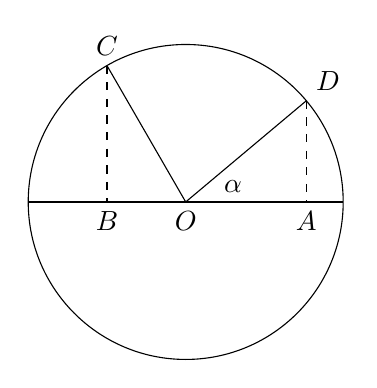
\begin{tikzpicture}[scale=2]
	\draw (0 , 0) circle (1);
	\draw (-1 , 0) -- (0 , 0) node[below]{$O$} -- (1 , 0);
	\draw [dashed](40:1)node[above right]{$D$} -- ({cos(40)} , 0)node[below]{$A$};
	\draw [dashed](120:1)node[above]{$C$} -- ({cos(120)} , 0)node[below]{$B$};
	\draw (0 , 0) -- (120:1);\draw (0 , 0) -- (40:1);
	\draw (0 . 3 , 0 . 1) node{$\alpha$};
\end{tikzpicture}


应用三角恒等式
\[
2 \cos 3 \alpha=8 \cos ^{3} \alpha-6 \cos \alpha
\]
而且令 $x=2 \cos \alpha$ ,  则有
\[
2 \cos 3 \alpha=x^{3}-3 x
\]
因为 $3 \alpha=120^{\circ} ,  \cos 3 \alpha=-1 / 2 ;$ 所以上面的方程式可以写作
\[
x^{3}-3 x+1=0
\]
这正是我们以前讨论过的方程式 . 

现在假说所给的只有单位长 , 我们可以作出一个半径是单位 长的圆 , 而且可以作 $O B=1 / 2$ ,  于是 $\angle A O C=120^{\circ}$ 因为所给的只
有单位长 , 所以我们的数域当限定是有理数域 . \footnote{因为从 $1$ 单用四种有理运算 ,  我们可以作出一切有理数 ,  即有理数域 . }

所以要解这个方程式 , 必须将一个立方根加入于有理数域中\footnote{参看前面几页 . } . 然而一个立方根是不能用直尺与圆规作出的 . 这样 , 我们可以知道: 用直尺与圆规三等分任意角是不可能的 . 

以相似的方法 , 不难证明用直尺、圆规解决立方倍积问题也是不可能的 . 对于这个问题 , 方程式是
\[
x^{3}=2
\]
数域是有理数域 . 这方程式在这个数域中的群含有六个置换 . 读者当证明须加入一个平方根和一个立方根于有理数域中 , 方程式的群才会变成 $1$  . 又因一个立方根是不能用直尺、圆规作出的 , 所以我们这个立方倍积问题是不可能的 . 

仿此 , 我们可以应用群论去探讨正多边形作图的问题\footnote{参考 L . E . Dickson: Modern Algebraic Theories ,  Chapter XI . } . 

\section{伽罗瓦的鉴定为什么是对的}

现在我们要证明一个方程式若有一个可解群 , 这方程式就可用根式解\footnote{我们不征此处证明这定理的逆定理 . 关于此点 , 读者可参考 L .  E .  Dickson:
	Modern Algebraic Theories , p . 198 . } . 

每个人在他少年的时候也许都有过这个经验: 想应运方程式
的根与系数之类系去解方程式 . 例如在二次方程式
\[
x^{2}+b x+c=0
\]
的两个根 $x_{1} ,  x_{2}$ 中 , 我们知道有
\[
x_{1}+x_{2}=-b \quad (1)
\]
与
\[
x_{1} x_{2}=c \quad (2)
\]
的关系 . 那末 , 我们为什么不从这两个方程式中去解 $x_{1} ,  x_{2}$ 呢? 我 们很容易发见这条路是走不通的 , 因为如果从(1)中得出 $x_{1}$ 的值 . 而后代入(2)中 , 结果是
\[
x_{2}^{2}+b x_{2}+c=0 , 
\]
这正与原来的二次方程式丝毫也没分别 . 所以这个法子只令我们兜了一个圈子又回到原来的出发点去了 . 但是 , 如果我们能得到一对都是一次的方程式 , 那末 ,  $x_{1}$ 和 $x_{2}$ 就实实在在可以求得了\footnote{但须假定这对方程式的系数之行列式不等于零 . } . 

如果方程式的群是一个元数为质数的巡回正置换群 , 那末 , 这方程式的确可以照刚才所说的法子去解 . 这一点我们立刻就要说明 , 而且我们还要观察这个特殊情形与一般的有可解群的方程式有什么关系 . 

现在先就这特殊情形来考究 , 设方程式
\[
f(x)=0
\]
有 $n$ 个相异的根 , 而且在那个由方程式的系数及 $1$ 之 $n$ 个 $n$ 次根决定的数域中\footnote{凡数域都含有一切有理数 , 因为我们若取数域中的任意一数来除他自己 ,  即得$1$  . 从 $1$ 应用有理运算 , 可得一切有理数 . 所以在任何数域中都含有一切有理数 . } , 此方程式的群是一个元数为质数的 巡回正置换群 . 

在此我们先要问什么叫做 1 之 $n$ 个 $n$ 次根 . 我们都知道 1 有 三个立方根\footnote{因为 $x^{3}=1 $ 可以写作$x^{3}-1=0$或$(x-1)\left(x^{2}+x+1\right)=0 , $由此即易得这三个根 . }
\[
1 , -\frac{1}{2}+\frac{1}{2} \sqrt{-3} , -\frac{1}{2}-\frac{1}{2} \sqrt{-3} . 
\]
(通常都记作 $1 ,  \omega ,  \omega^{2}$ )仿此 , 在一般的情形 ,  $1$ 有 $n$ 个 $n$ 次根 , 这 $n$个 $n$ 次根我们记作
\[
1 ,  \rho ,  \rho^{2} ,  \cdots ,  \rho^{n-1}
\]
1 的三个立方根只包含有理数和有理数的 根数 , 同样 $1$ 的 $n$ 个次根也只包含有理数和有理数的根数 . 所以这种数加入数域中去 时并不影响到“方程式是能用根式解”的这句命辞 . 

因为我们假定这方程式的群是一个元数为质数的巡回正置换群 , 群中的元素都是置换
\[(123……n)\]
的乘幂 , 这个置换的$n$次乘幂就是不动置换\footnote{见前面几页 . } . 

现在我们要应用一组一次方程式
\[
x_{1}+\rho^{k} x_{2}+\rho^{2 k} x_{3}+\cdots+\rho^{(n-1) k} x_{n}=\gamma_{k} , \quad (3)
\]
此处 $k$ 的值得为 $0$ 与 $n-1$ 间之任何整数 , 所以这是将 $n$ 个方程式
写作一个的简便写法 . 例如当 $k=0$ 时 , $(3)$就成为
\[
x_{1}+x_{2}+x_{3}+\cdots \cdots+x_{n}=\gamma_{0}
\]
当 $k=1$ 时 ,  $(3)$成为
\[
x_{1}+\rho x_{2}+\rho^{2} x_{3}+\cdots \cdots+\rho^{n-1} x_{n}=\gamma_{1}
\]
等等 . 

因为一个方程式的最高次项系数若是 $1$ , 则诸根之和等于方程式中第二项的系数的负值 , 所以 $\gamma_{0}$ 之值可以直接从方程式的系数中求得 . 现在要将置换
\[
(123 \cdots n)
\]
施行于$(3)$的左端 ,  $(3)$式左端就成为
\[
x_{2}+\rho^{k} x_{3}+\rho^{2 k} x_{4}+ \cdots+\rho^{(n-1) k} x_{1}
\]
但是若将$(3)$式左端用 $\rho^{-k}$ 一乘 , 也可得出同样的结果 , 这是因为
$\rho^{n}=1$ 的缘故 . 所以置换
\[
(123 \cdots n)
\]
将 $\gamma_{k}$ 之值变为 $\rho^{-k} \gamma_{k}$ .  又因 $\rho^{n}=1$ ,  故 $\left(\gamma_{k}\right)^{n}=\left(\rho^{-k} \gamma_{k}\right)^{n}$ ,  所以置换
\[
(123 \cdots \cdots n)
\]
不变更 $\gamma_{k}^{n}$ 的值 . 同样 , 群中其他的置换也不变 $\gamma_{k}^{n}$ 之值\footnote{因为这群是巡回群 , 群中的置换都是$(123\cdots n)$的乘幂 , 所以将群中某一置换施行于 $\gamma_{k}^{n}$ 实在就相当于将 $(123 \cdots n)$ 重复施行若干次于 $\gamma_{x_{\circ}}^{n}$ 但将 $(123 \ldots n)$施行一次于$\gamma_{x}^{n}$ 既不改变 $\gamma_{x}^{n}$ 的值 , 重复施行若干次当然也不变更 $\gamma_{x}^{n}$ 的值} . 

如此 , 群中一切置换既然都不变更 $\gamma_{k}^{n}$ 之值 ,  $\gamma_{k}^{n}$ 之值必在那数域中\footnote{参看前面几页 . } . 因此 ,  $\gamma_{k}$ 是数域中某一个数的 $n$ 次根 . 这就是说: 所有 $\gamma$ 的值都可由根式得到(对于那数域而言!) . 而由 $(3)$ 中可以将$x$ 用 $\rho$ 与 $\gamma$ 表出 , 于是这组方程式$(3)$是可以用根式解的 . 但是这些 $x$ 就是方程式 $f(x)=0$ 的根 . 所以我们已经证明: 如果方程式在一个数域中的群是元数为质数的巡回正置换群 , 则此方程式必可用根式解 . 

举例来说: 方程式
\[
x^{3}-3 x+1=0
\]
在有理数域中的群是 $1 ,  (123) ,  (132)$\footnote{参看前面几页 . }; 这是一个元数为质数的 巡回正置换群 , 所以我们可以从
\[
\begin{array}{c}
	x_{1}+x_{2}+x_{3}=0 \\
	x_{1}+\omega x_{2}+\omega^{2} x_{3}=\gamma_{1} \\
	x_{1}+\omega^{2} x_{2}+\omega x_{3}=\gamma_{2}
\end{array}
\]
这三个一次方程式中解它 . 此处 $\omega$ 表示 $1$ 的一个虚立方根 , $\gamma_{1}$ 与$\gamma_{2}$ 可以由数域中的数的根数而得 . 换句话说 , 如果把这种根数加入到数域中去 , 则 $x$ 都存在于扩大的数域中 . 

但是 , 假使方程式的群不是一个元数为质数的巡回正置换群 , 那又怎么样呢?

方程式的群是一个可解群时 , 他的解法在第 35 页中已说了一 个梗概 . 在那里我们已经知道: 假使组合因数都是质数 , 虽则方程式的群不是一个元数为质数的巡回正置换群 , 这方程式还是能用根式解的 . 因为这时候每个辅助方程式在那个用前几个辅助方程式的根扩大成的数域中的群是一个元数为质数的巡回正置换群 . 

如此 , 每个辅助方程式既有一个元数为质数的巡回正置换群 ,  根据以前所说的 , 这些辅助方程式都能用根式解 . 所以这些加入原来的数域去的辅助方程式的根 , 都只不过是原来的数域中的数的根数而已 . 这样看来 , 只要方程式的群是可解群 , 这方程式就是能用根式解的 . 

在一般的情形 , 我们常可以取
\[
y^{2}=\left(x_{1}-x_{2}\right)^{2}\left(x_{1}-x_{3}\right)^{2}  \cdots \left(x_{n-1}-x_{n}\right)^{2}
\]
作第一个辅助方程式 , 此式右端是所有每两个根之差的平方之积 . 假若方程式的第一项系数是 $1$ 的话 , 那末 , 上式的右端正是方程式的\emph{判别式}(Discriminant) . 例如二次方程式
\[
x^{2}+b x+c=0
\]
的两个根 $x_{1} ,  x_{2}$ 之差之平方是
\[
\left(x_{1}-x_{2}\right)^{2}=\left(x_{1}+x_{2}\right)^{2}-4 x_{1} x_{2}=b^{2}-4 c
\]
这恰是方程式的判别式 . 同样 , 高次方程式的判别式也可从系数求得 . 现在第一个辅助方程式的两个根就是这判别式的两个平方根 , 将这两个平方根加入数域中 , 方程式在这新的数域 $F_{1}$ 中的群是 $H$ .  我们再照同样方法用其余的辅助方程式进行下去 . 

设若所要解的方程式是一个一般的三次方程式 , 将第一个辅助方程式的根加入原来的数域之盾 , 方程式的群变为 $H_{\circ}$ 在这情形 ,  $H$ 是一个元数为质数的巡回正置换群 . 所以我们可以利用
\[
\begin{array}{r}
	x_{1}+x_{2}+x_{3}=-b \\
	x_{1}+\omega x_{2}+\omega^{2} x_{3}=\gamma_{1} \\
	x_{1}+\omega^{2} x_{2}+\omega x_{3}=\gamma_{2}
\end{array}
\]
这三个一次方程式来解原来的三次方程式 . 此中的 $\gamma_{1} ,  \gamma_{2}$ 可由数域(这数域是由三次方程式的系数以及第一个辅助方程式的根而决定的)中的数之根数求得\footnote{参考 L . E . Dickson:Modem Algebraic Theories , p  . 136 . 但此处的$\gamma_{1} ,  \gamma_{2}$该书中记作$\fi \psi $} . 换句话说 , 假使把 $\gamma_{1} ,  \gamma_{2}$ 的值也加入数域中 , 则方程式的群变为 $1$  . 这也就是说 ,  $x_{1} ,  x_{2} ,  x_{3}$ 存在于这个最后经 $\gamma_{1} ,  \gamma_{2}$ 之加入而扩大成的数域中 . 

如此我们已经证明: 方程式在一个由其系数与 $1$ 之 $n$ 个 $n$ 次根而决定的数域中的群若是一个可解群 , 则此方程式是可以用根式解的 . 

当然 , 如果方程式在一个含有其系数的数域中的群是可解群 ,  则对于这数域而言 , 此方程式是可以用根式解的 .  本书所说的已够使读者知道一个大概 , 我们希望读者继续去 研究这门引人入胜的数学 . 要知道用群论解方程式并不是这个令 人惊叹的群的概念的惟一应用 . 

应用群论于几何学\footnote{参考 Veblen and Young:Projective Geometry . } , 使几何学起了一个大的改革 . 还有在 相对论中 , 群论也极重要 . 培尔(E .  $\mathrm{T}  .  \mathrm{Bell}$ )说过\footnote{参看 E . T . Belk:The Queen of the Sciences 及 C . J . Keyser: Mathematical Philosophy 一书中论群之概念一章 . } “无论在什么地方 ,  只要能应用群论 , 从一切纷乱混淆中立刻结晶出简洁余和谐 .  群的概念是近世纪科学思想的出色的新工具之一 . ”

\section{要义}
1 . 数学并不像普通一般人所相信的 , 仅是一组呆板的定义和 法则 . 在把人们的心从他的偏见和旧的定义中解放出来以后 , 现 代的数学已开辟了一块非常膏腴的园地(参阅第95-98页) . 

2 . 不过这种解放绝对不是纷乱无主的 , 在推广了定义、选定 了公理和确定了数域以后 , 我们就要遵从这些限制 , 只要我们在这 一个系统里研究的话 , 对于他们就要表示忠诚(参阅第89—91页) . 

3 . 然则 , 在起初的 时候我们将如何选择那 些公理和定义以及数域 呢 , 那是要看目的如何 而定的 . 如伽罗瓦的目 的是要用既定的方法来 解方程式(参阅第88— 91 页) . 

4 . 有了目的 , 有了 和这目的契合的公理 ,  那末 , 方法又怎样呢? 这方法就是要用一个以 一些变化作元素的群之 元素来变化那些我们所 研究的东西 , 并且找出 对于这些变化不会更易的东西 , 这些在我们的 系统中是不会变更的 . 

5 . 从现代数学中可以得到的另一个训示是:一个很小的原因 可以引起惊人的结果 . 这正是:“星星之火 , 可以燎原” . 一个问题 可以是可能的或不可能的 , 只要在条件上有点轻微的变更(参阅第 90-91页) . 这个拿几何学最好做比喻:只在一条公理上有一点 细微的变化 , 把其余的公理照旧 , 就把欧几里得几何学变成非欧几 里得几何学了\footnote{参看本书作者所著之 Non-Euclidian Geometry or Three Moons in Mathesis 一书 . } . 


\chapter{附录方程解法}

代数方程式是
\[
a_{0} x^{n}+a_{1} x^{n-1}+\cdots \cdots+a_{n}=0
\]
的形式的方程式 ,其中 $n$ 是正整数 .

一次方程式
\[
a x+b=0.
\]


二次方程式
\[
a x^{2}+b x+c=0.
\]


三次方程式
\[
a x^{3}+b x^{2}+c x^{2}+d=0.
\]

四次方程式
\[
a x^{4}+b x^{3}+c x^{2}+d x+e=0.
\]


\section{一次方程解法}

一次方程式:
\[
a x+b=0
\]

当$a \neq 0$时:
\[
x=-\dfrac{b}{a} . 
\]

当$ a = 0 , b \neq 0 $ 时:
原方程无解 . 


当$ a = 0 , b = 0 $ 时:
原方程有无数解 . 


\section{二次方程解法}

\subsection{现行课本常见的推导}
现在各通行课本对一元二次方程求根公式的推导 , 一般是通过配方法得到的 , 即:

对于方程 $ax^{2}+bx+c=0(a \neq 0)$

(1)方程两边同除以 $a$ ,得: $x^{2}+\frac{b}{a} x+\frac{c}{a}=0$

(2)将常数项移到方程的右边,得: $x^{2}+\frac{b}{a} x=-\frac{c}{a}$

(3)方程两边同时加上 $\left(\frac{b}{2 a}\right)^{2}$ ,得: 
$x^{2}+\frac{b}{a} x+\left(\frac{b}{2 a}\right)^{2}=\left(\frac{b}{2 a}\right)^{2}-\frac{c}{a}$

(4)左边配成完全平方式 , 右边通分,得:
$\left(x+\frac{b}{2 a}\right)^{2}=\frac{b^{2}-4 a c}{4 a^{2}}$

由 $a \neq 0$ 得, $4 a^{2}>0$, 
所以 , 当 $b^{2}-4 ac \geq 0$ 时, $\frac{b^{2}-4 a c}{4 a^{2}} \geq 0$,

所以, $x=\frac{-b \pm \sqrt{b^2-4 a c}}{2 a}$

\subsection{另外一种推导}
$a x^{2}+b x+c=0(a \neq 0)$

方程两边同乘以 $4a$ ,得: $4a^{2} x^{2}+4 abx+4 ac=0,$

方程两边同时加上 $b^{2}$ ,得: $4 a^{2} x^{2}+4 abx+4ac+b^{2}=b^{2},$

把 $4 a c$ 移到方程的右边,得: $4a^{2} x^{2}+4abx+b^{2}=b^{2}-4ac,$

将左边配成完全平方式,得: $(2 a x+b)^{2}=b^{2}-4 a c,$

当 $b^{2}-4ac \geq 0$ 时 , 有:
$2 a x+b=\pm \sqrt{b^{2}-4 a c}.$

所以, $2 ax=-b \pm \sqrt{b^{2}-4 a c}.$

因为, $a \neq 0,$

所以, $x=\frac{-b \pm \sqrt{b^2-4 a c}}{2 a}.$

\subsection{Vieta的推导}
引自:古今数学思想 , 克莱因 , 第一册 . 

Cardan, Tartaglia, Ferrari通过解出三次和四次方程的许多 例子 , 表明他们曾寻求并获得能用之于一切情况的求解三次和四 次方程的方法.注重一般性是一种新的特色.他们的工作做在 Vieta引用文字系数之前 , 所以不能利用这个工具.Vieta在创用 文字系数之后使证明有可能获得普遍意义 , 又进而追求另一类普遍性.他发现解二次、三次和四次方程的方法很不相同 , 就想找一 种能适用于各次方程的方法.他的头一个想法是用置换法消去比 最高次项次数小一次的项.Tartaglia对三次方程以海做了 , 但并 未对所有方程都这样试做过.

Vieta在他的《分析术引论》中做了如下的步骤:为解二次方程
\[
x^{2}+2 b x=c
\]
他让
\[
y=x+b
\]
于是
\[
y^{2}=x^{2}+2 b x+b^{2}
\]
利用原方程,得
\[
y=\sqrt{c+b^{2}}
\]
于是
\[
x=y-b=\sqrt{c+b^{2}}-b
\]

拓展:

对于三次方程
\[
x^{3}+b x^{2}+c x+d=0
\]
Vieta 先设 $x=y-b / 3 .$ 置换结果得的简三次方程
\[
y^{3}+p y+q=0 \quad (23)
\]
其次他再作一次变换, 那就是如今在学校里所教的. 就是令
\[
y=z-\frac{p}{3 z} \quad (24)
\]
得
\[
z^{3}-\frac{p^{3}}{27 z^{3}}+q=0
\]
然后他解出这 $z^{3}$ 的二次方程, 得
\[
z^{3}=-\frac{q}{2} \pm \sqrt{R}, \text { 其中 } R=\left(\frac{p}{3}\right)^{3}+\left(\frac{q}{2}\right)^{2}
\]
这里也同 Cardan 的方法一样, 有两个 $z^{3}$ 的值. Vieta 虽然只用了
$z^{3}$ 的正立方根 , 但我们可以用所有六个(复数)根. 应用(24)的结
果可以证明从六个 $z$ 值只能得出三个不同的 $y$ 值.
为解一般四次方程
\[
x^{4}+b x^{3}+c x^{2}+d x+e=0
\]
Vieta 设 $x=y-b / 4$ 于是把方伸化为
\[
x^{4}+p x^{2}+q x+r=0
\]
然后他把末后三项移到右边并在两边加上$2x^2y^2+y^4$.这就使左
边配成完全平方, 然后也象 Ferrari 的方法那样, 适当选取$y$ , 使右
边成为形如 $(A x+B)^{2}$ 的完全平方. 为选取合适的 $y$, 他利用二次
方程的判别式条件, 得出 $y$ 的一个六次方程而且凑巧还是 $y^{2}$ 的三 次方程 . 这一步以及其余各步就完全和 Ferrari 的方法一样了.

Vieta 所探求的另一个一般性方法是把多项式分解成一次因
子 , 如同我们把 $x^{2}+5 x+6$ 分解成 $(x+2)(x+3)$ 那样. 这事他没
有做成功, 部分原因是他只取正根而舍弃其他一切根,部分原因是
他没有足够的理论(如分解因子定理)作为依据来搞出一般方法.
Thomas Harriot 也有同样的想法但也由于同样的原因而片于失
败.

寻求一般代数方法的工作接着就转向解四次以上的方程.
James Gregory 在提出他自己的解三次及四次方程的方法后 , 便 
试图用这些方法来解 五次方程 . 他和 Ehrenfried Walter von
Tschirnhauson $(1651 \sim 1708)$ 想通过变换把高次方程化为只含 $x$
的一个乘幂和一个常数那么两项的方程. 解四次以上的方程的这
些尝试都失败了. Gregory 在其后关于积分法的著作中猜测 , 对
$n>4$ 的一般 $n$ 次方程是不能用代数方法求解的 . 

\section{三次方程解法}

卡尔达诺(1501年9月24日 ~1576年9月21日)是大利文艺复兴时期百科全书式的学者 , 他最著名的成就是推导出了三次代数方程的解法 , 即卡尔达诺公式 . 

\subsection{思想}
先把方程 $a x^{3}+b x^{2}+c x+d=0 \quad (1)$ 
化为 $x^{3}+p x+q=0 \quad (2)$ 的形式 , 再直接利用卡尔丹诺公式.


\subsection{Cardan的方法}
引自:古今数学思想 , 克莱因 , 第一册 . 

用配方法解二次方程是从巴比伦时代就已经知道的 , 从那时
起直到 1500 年, 这方面的唯一进展 是印度人作出的 , 他们把 
$x^{2}+3 x+2=0$ 与 $x^{2}-3 x-2=0$ 那样的二次方程作为同一类型来
处理 , 而他们的前人乃至文艺复兴时期的绝大多数后继者却宁
愿把后一个方程作为 $x^{2}=3 x+2$ 的形式来处理. 如前所指出的 ,  
Cardan 确曾解出一个有复数根的二次方程, 但他认为这些解是无
用的而未加考虑. 至于三次方程 , 则除了个别情形之外数学家还
对之束手无策; 直到 1494 年那么晚近的年月, Pacioli 还宣称一般
的三次方程是不可能解的 . 

1500 年左右, 波仑亚(Bologna)的数学教授 Scipione dal Ferro
$(1465 \sim 1526)$解出了 $x^{3}+m x=n$ 类型的三次方程. 但他没有发表
他的解法, 因在十六和十七世纪时 , 人们常把所得的发现保密 , 而
向对手们提出挑战, 要他们解出同样的问题. 但在 1510 年左右,
他确曾把他的方法秘传给 Antonio Maria Fior (十六世纪前半叶)
和他的女婿兼继承人 Annibale della Nave$(1500 ? \sim 1558) .$
直到布里西亚(Brescia)的 Niccolò Fontana $(1499 ? \sim 1557)$ 出 
场之前 , 情況没有什么变化. 这人在孩提时被一个法国兵用马刀
砍伤脸部而引起口吃;因此大家称他为 Tarvaglia, 意即‘口吃者’.
他出身贫寒 , 自己学会拉丁文、希腊文和数学.他靠着在意大利各
城市讲授科学谋生. 1535 年, Fior 向 Tartaglia 挑战 , 要他解 三 
十个三次方程. Tartaglia 说他早已解出了 $x^{3}+m x^{2}=n(m$ 与 $n$ 是 
正数)类型的三次方程 , 这次解出了所有三十个方程 , 其中包括 $x^{3}+m x=n$ 类型的方程.

在Cardan的恳切要求之下 , 并发誓对此保守秘密 , Tartaglia
オ把他的方法写成一首语句晦涩的诗告诉给 Cardan. 这是 1539
年的事. 1542 年 Cardan 和他的学生Lodovioo Ferrari $(1522 \sim 1565)$
在 della Nave 访问他们的时候 , 肯定认为 dal Ferro 的方法同
Tartaglia 的方法是相同的. Cardan 不顾他的誓言, 把他对这个方
法的叙述发表在他的《重要的艺术》里. 他在第十一章里说: “波仑
亚的 Scipio Ferro 差不多在三十年以前就发现了这个法则 , 并把
它传给威尼斯 (Venice)的 Antonio Maria Fior, Fior 在他与布里
西亚的 N. Tartaglia 竞赛的时候使 Tarfäglia 有机会发现这一法
则 . 我在获得这种帮助的情况下找出了它的各种形式的证明. 这是很
难做的. 我把它叙述如下 . ”

Tartaglia 抗议 Cardan 背信弃义. 并在《各种问题与发明》
(Quesiti ed invenzioni diverse, 1546 ) 中发表了他自己的方法. 但
是无论在这本书中还是在他的《数量概论》 (1556) (这是阐释那个
时代的算术知识和几何知识的一本好书)中, 他都没有给出关于三
次方程本身的更多材料. 关于谁先解出三次方程的争议使 Tartag
lia 与 Ferrari 发生公开冲突 , 最后以双方肆意谩骂而 告终 , 但
Cardan 并未参与其中. Tartaglia 自己也不是无可非议的; 他 出
版了 Archimedes 的一些著作的译本 , 实则 是抄自 William of
Moerbecke(卒于 1281 年左右)的 , 并且他自称发现了物体沿斜面 
运动的规律, 但实际上这是 Jordanus Nemorarius 创立的.


在 Cardan 所发表的方法中 , 他先以 $x^{3}+6 x=20$ 为例 . 但为
说明这个方法的一般性, 我们来考察
\[
x^{3}+m x=n, \quad (4)
\]
其中 $m$ 与 $n$ 是正数. Cardan 引入 $t$ 与 $u$ 两个量, 并令
\[
t-u=n, \quad (5)
\]
以及
\[
(t u)=\left(\frac{m}{3}\right)^{3}, \quad (6)
\]
然居他断言
\[
x=\sqrt[3]{t}-\sqrt[3]{u}, \quad (7)
\]
他利用(5)及 (6)进行消元并解所得的二次方程, 得出

\[t=\sqrt{\left(\frac{n}{2}\right)^{2}+\left(\frac{m}{3}\right)^{3}}+\frac{n}{2}, \quad u=\sqrt{\left(\frac{n}{2}\right)^{2}+\left(\frac{m}{3}\right)^{3}}-\frac{n}{2}, \quad (8).\]

这里我们也象 Cardan 那样取正根 . 求出了 $t$ 和 $u$ 后, Cardan
取两者的正立方根 , 并用(7)给出 $x$ 的一个值. 据认为这就是Tartaglia所得出的同一个根.

以上是 Cardan 发表的方法. 不过他得证明 $(7)$ 给出的是 $x$ 的 
一个正确的值. 他的证明是用儿何方法的; Cardan 把 $t$ 和 $u$看成 
立方体的体积, 其边长各为 $\sqrt[3]{t}$ 和 $\sqrt[3]{u}$,而乘积 $\sqrt[3]{t} \sqrt[3]{u}$ 是两边所 
形成的矩形 , 其面积为 $m / 3 .$ 又, 我们所说的 $t-u=n$ 对 Cardan
说是两个体积之差等于 $n_{0}$ 于是他说解 $x$ 就等于两立方体边长之 
差, 即 $x=\sqrt[3]{t}-\sqrt[3]{u}$. 为证明这 $x$ 值是对的, 他叙述并证明一个 
几何引理, 这就是: 若从一根线段 $A C$ 上截去一段 $B C$, 则 $A B$ 上的立方体等于 $A C$ 上的立方体减去 $B C$ 上的立方体再减 去
以 $A C, A B$ 及 $B C$ 为边的正平行六面体、这个几何引理的内容当 
然只不过是说

\[\quad(\sqrt[3]{t}-\sqrt[3]{u})^{3}=t-u-3(\sqrt[3]{t}-\sqrt[3]{u}) \sqrt[3]{t} \sqrt[3]{u} \quad (9)\]

有了这个引理(应用二项式定理 , 我们知道这引理必然 成立 , 但
Cardan 是引用 Euclid 书中的定理来证明的), Cardan 就只要证 
明: 若设 $x=\sqrt[3]{t}-\sqrt[3]{u}, t-u=n$ 以及 $\sqrt[3]{t} \sqrt[3]{u}=\frac{m}{3}$, 则从引
理便得 $x^{3}=n-m x .$ 于是, 如果他选取了 $t$ 和 $u$ 使之能满足条件
$(5)$与 $(6)$, 则 $(7)$ 所给出的以 $t$ 与 $u$ 表达的 $x$ 值就能满足三次方
程. 然后他纯粹用语言叙述这方法的算术规则, 告诉我们怎样按
照 $(8)$ 用 $m$ 及 $n$ 表 $t$ 及 $u$ 并作出 $\sqrt[3]{t}-\sqrt[3]{u} .$

Cardan (还有 Tartaglia)又解出了下列三种特殊类型的方程:
$x^{3}=m x+n, \quad x^{3}+m x+n=0, \quad x^{3}+n=m x .$
他需要把这三种情形都分别处理 , 并且把三者同方程(4) 分别 处
理, 原因是, 第一, 那时候欧洲人写的方程中只含正数的项; 第二 , 
他得对每种情形所用的法则分别给出几何上的说明.

Cardan 还给出怎样解 $x^{3}+6 x^{2}=100$ 这类方程的方 法. 他知
道怎样消去 $x^{2}$ 项; 即, 由于该项的系数是 6, 他以 $y-2$ 代 $x$, 得出
$y^{3}=12 y+84 .$ 他还指出象 $x^{6}+6 x^{4}=100$ 这样的方程在设 $x^{2}=y$
后可作为三次方程来处理. 他在书中自始至终都给出正根和负
根 , 尽管他把负数称作虚拟的数. 但对复数根他是略而 不提的.
事实上, 他在第 37 章中把那些既不解出真根(正数根) 又不能解出
假根(负数根)的问题称作错题. 书讲得很详细——对现代读者来
说甚至腻人,——因为 Cardan 把许多情形(不仅是对于三次方程,
而且对于那些为求 $t$ 及 $u$ 而必须解出的辅助二次方程)都一一分
别处理. 在每种情形下, 他把方程都写成各项有正系数的形式.


\subsection{Vieta的解法}
引自:古今数学思想 , 克莱因 , 第一册 . 

Vieta 在他著于 1591 年并出版于 1615 年的《论方程的整理与
修正》(De Aequationum Recognitione et Emendatione) 中, 已能
用一个三角恒等式解出了不可约三次方程 , 从而避免使用 Cardan 的公式. 这个方法如今还在用. 他从下列恒等式开始:
\[
\cos 3 A \equiv 4 \cos ^{3} A-3 \cos A \quad (10)
\]
令 $z=\cos A$, 这恒等式就变为
\[
z^{3}-\frac{3}{4} z-\frac{1}{4} \cos A \equiv 0 \quad (11)
\]
设所给三次方程是(Vieta 处理的是 $x^{3}-3 a^{2} x=a^{2} b$  , 其中 $a>b / 2$)
\[
y^{3}+p y+q=0 .  \quad (12)
\]
代入 $y=n z$, 其中 $n$ 可按需要指定, 便可使(12)的系数化成同(11) 
的系数一样. 将 $y=n z$ 代入(12) , 得
\[
z^{3}+\frac{p}{n^{2}} z+\frac{q}{n^{3}}=0 \quad (13)
\]
现在我们需要取 $n$ 使 $p / n^{2}=-3 / 4$, 故
\[
n=\sqrt{-4 p / 3} \quad (14)
\]
选取了这个 $n$ 值后, 再取 $A$ 值使
\[
\frac{q}{n^{3}}=-\frac{1}{4} \cos 3 A \quad (15)
\]
也就是使
$(16)$
\[
\cos 3 A=-\frac{4 q}{n^{3}}=\frac{-q / 2}{\sqrt{-p^{3} / 27}}
\]

我们可证明: 若三根是实数 , 则 $p$ 是负数 , 因而 $n$ 是实数. 又因
$|\cos 3 A|<1$, 故可从三角函数表查出 $3 A$.

不管 $A$ 取何值, $\cos A$ 总满足(11), 因(11)是个恒等式. 现已
选取 $A$ 使(13)成为(11)的特例. 对于这个 $A$ 值, $\cos A$ 满足 (13).
但 $A$ 值是由 (16) 确定的 , 而这 $A$ 又埔定了 $3 A$. 但若 $A$ 是满足
(16)的任一值, 则 $A+120^{\circ}$ 及 $A+240^{\circ}$ 也满足(16). 因 $z=\cos A$,
故有三个值满足(13);
\[
\cos A, \cos \left(A+120^{\circ}\right) \quad , \cos \left(A+240^{\circ}\right) .
\]
满足(12)的那三个值是 $z$ 值的 $n$ 倍, 而 $n$ 是由(14)给出的. Vieta
得出的只是一个根.

三次方程当然有三个根. 对 Cardan 的三次方程解法的第一个
完整的讨论是 1732 年由 L. Euler 作出的 , 他强调指出三次方程
总有三个根, 并指出怎样去求.若 $\omega$ 和 $\omega^{2}$ 是 $x^{3}-1=0$ 的复数根,
也就是说, 是 $x^{2}+x+1=0$ 的根, 则 $(8)$ 中 $t$ 和 $u$ 的三个立方根是
\[
\sqrt[3]{t}, \omega \sqrt[3]{t}, \omega \sqrt[2]{t} \quad \text { 和 }  \quad \sqrt[3]{u}, \omega \sqrt[3]{u}, \omega^{2} \sqrt[3]{u}
\]

现在必须从第一组里选取一根, 从第二组里选取一根, 使两者的乘 积是实数 $m / 3$. (参看 Cardan 解法中的方程(6).) 因 $\omega$ 与 $\omega^{2}$ 是 1
的立方根, $\omega \cdot \omega^{2}=\omega^{3}=1$; 故据 $(7)$ 可知合适选取的 $x$ 应为

$\left\{
\begin{array}{l}
	x_{1}=\sqrt[3]{t}-\sqrt[3]{u}, \\
	x_{2}=\omega \sqrt[3]{t}-\omega^{2} \sqrt[3]{u},  \quad (17)\\ 
	x_{3}=\omega^{2} \sqrt[3]{t}-\omega \sqrt[3]{u}
\end{array}\right.$

三次方程成功地解出之后接着几乎立即成功地解出了四次方
程. 解法是 Lodovico Ferrari 给出的并发表在 Cardan 的《重要的
艺术》中; 这里我们用现代的记号把它写出来并用文字系数以示其
普遍性. 设方程是

$x^{4}+b x^{3}+c x^{2}+d x+e=0 . \quad (18)$

移项后得

$x^{4}+b x^{3}=-c x^{2}-d x-e. \quad (19)$

在左边加上 $\left(\frac{1}{2} b x\right)^{2}$ 配成平方. 得

$\left(x^{2}+\frac{1}{2} b x\right)^{2}=\left(\frac{1}{4} b^{2}-c^{2}\right) x^{2}-d x-e . \quad (20)$

两边再加上 $\left(x^{2}+\frac{1}{2} b x\right) y+\frac{1}{4} y^{2}$, 得

$\left(x^{2}+\frac{1}{2} b x\right)^{2}+\left(x^{2}+\frac{1}{2} b x\right) y+\frac{1}{4} y^{2}
=\left(\frac{1}{4} b^{2}-c+y\right) x^{2}+\left(\frac{1}{2} b y-d\right) x+\frac{1}{4} y^{2}-e \quad (21)$

若使右边这个 $x$ 的二次式的判别式等于零 , 就能使这一边成为 $x$
的一次式的完全平方. 于是设

$\quad\left(\frac{1}{2} b y-d\right)^{2}-4\left(\frac{1}{4} b^{2}-c+y\right)\left(\frac{1}{4} y^{2}-e\right)=0.(22)$

这是 $y$ 的一个三次方程. 选取这三次方程的任一个根代入(21)中
的 $y$. 根据左边也是个完全平方这一事实, 取平方根, 得到 $x$ 的一 
个二次式, 它等于 $x$ 的两个互为正负的线性函数之一. 解出这两
个二次方程便得到 $x$ 的 4 个根. 若从(22)选取另一个根就会从
(21)引出一个不同的方程但得到同样的四个根.

对于三次方程
\[
x^{3}+b x^{2}+c x+d=0,
\]
Vieta 先设 $x=y-b / 3 .$ 置换结果得约简三次方程
\[
y^{3}+p y+q=0 .(23)
\]
其次他再作一次变换, 那就是如今在学校里所教的. 时是令
\[
y=z-\frac{p}{3 z},(24)
\]
得
\[
z^{3}-\frac{p^{3}}{27 z^{3}}+q=0.
\]
然后他解出这 $z^{3}$ 的二次方程, 得
\[
z^{3}=-\frac{q}{2} \pm \sqrt{R},  \quad \text { 其中 } \quad R=\left(\frac{p}{3}\right)^{3}+\left(\frac{q}{2}\right)^{2}
\]
这里也同 Cardan 的方法一样, 有两个 $z^{3}$ 的值. Vieta 虽然只用了
$z^{3}$ 的正立方根 , 但我们可以用所有六个(复数)根 . 应用(24)的结
果可以证明从六个 $z$ 值只能得出三个不同的 $y$ 值.











\subsection{思路分析}
对比以下两式:

$x^{3}+p x+q=0$

$(u+v)^{3}=u^{3}+3 u^{2} v+3 u v^{2}+v^{3}$

即:

$x^{3}+p x+9=0$

$(u+v)^{3}=3 u v(u+v)+u^{3}+v^{3}$

于是:

$x^{3}+p x+q=0$

$(u+v)^{3}-3 u v(u+v)-\left(u^{3}+v^{3}\right)=0$

如果能够设法找到$u,v$使得以上两式对应相等 , 那么3次方程就能够转换成一个最简单3次方程$X^3=0$的形式 . 

即:

$x=u+v$

$uv=-\dfrac{p}{3}$

$u^3+v^3=-q$

对$uv=-\dfrac{p}{3}$两边3次方 , 得$u^{3} v^{3}=-\left(\frac{p}{3}\right)^{3}$

对$u^3+v^3=-q$两边乘以$v^3$ , 得$ u^{3} v^{3}+\left(v^{3}\right)^{2}=-q v^{3}$

代入 , 整理 , 得:$\left(v^{3}\right)^{2}+q v^{3}-\left(\frac{p}{3}\right)^{3}=0$

这其实只是一个伪装过的2次方程 , 把$v^3$看成一个未知数 , 用2次求根公式求出$v^3$ , 然后两边开3次方根就得到:

$v^{3}=-\frac{q}{2} \pm \sqrt{\left(\frac{q}{2}\right)^{2}+\left(\frac{p}{3}\right)^{3}}$

$v=\sqrt[3]{-\frac{q}{2} \pm \sqrt{\left(\frac{q}{2}\right)^{2}+\left(\frac{p}{3}\right)^{3}}}$

在这几个式子里 , $u$和$v$是不可分割的 , 求$u$ , 得到的是同一个答案

$u,v=\sqrt[3]{-\frac{q}{2} \pm \sqrt{\left(\frac{q}{2}\right)^{2}+\left(\frac{p}{3}\right)^{3}}}$

现在答案有正负号 , 我们貌似对$u$和$v$每个都求出两个解 , 这样$u+v$就总共有3个可能 . 

两个都是减号 , 两个都是加号 , 一加一减 , 一减一加得出的是同一个答案 , 而3次方程正好至多有3个根

然后把这三个根带入方程 , 你会发现 , 只有一加一减才是3次方程的一般解 . 

于是$x=\sqrt[3]{-\frac{q}{2}-\sqrt{\left(\frac{q}{2}\right)^{2}+\left(\frac{p}{3}\right)^{3}}}+\sqrt[3]{-\frac{q}{2}+\sqrt{\left(\frac{q}{2}\right)^{2}+\left(\frac{p}{3}\right)^{3}}}$



\subsection{卡尔丹诺公式推导方法一}
将解方程 $a x^{3}+b x^{2}+c x+d=0 \quad (1)$ 

转化为解方程 $y^{3}+p y+q=0 \quad (2).$ 

不妨设 $p,q$ 均不为零, 令 $y=u+v \quad (3)$  

代入(2)得, $u^{3}+v^{3}+(u+v)(3 u v+p)+q=0 \quad (4)$

选择 $u,v$, 使得 $3 u v+p=0$, 即 $u v=-\frac{p}{3} \quad (5)$ 

代入(4) 得, $u^{3}+v^{3}=-q \quad (6) $ 

将(5) 式两边立方得, $u^{3} v^{3}=-\frac{p^{3}}{27} \quad (7)$

联立(6)、(7)两式 , 得关于 $u^{3}$ 、 $v^{3}$ 的方程组:

$\left\{
\begin{array}{l}
	u^{3}+v^{3}=-q ,  \\ 
	u^{3} v^{3}=-\frac{p^{3}}{27} , 
\end{array} \quad\right.$ 
且 $u v=-\frac{p}{3}$

于是问题归结于求上述方程组的解 , 即关于 $t$ 的一元二次方程 $t^{2}+q t-\frac{p^{3}}{27}=0$ 的两根 $u^{3}, v^{3}$  .  

设 $\Delta=q^{2}+\frac{4 p^{3}}{27}, \quad D=\frac{\Delta}{4}=\left(\frac{q}{2}\right)^{2}+\left(\frac{p}{3}\right)^{3}, \quad T=-\frac{q}{2}.$

又记 $u^{3}$ 的一个立方根为 $u_{1}$, 则另两个立方根为 $u_{2}=\omega_{1} u_{1}, u_{3}=\omega_{2} u_{1}$, 其中 $\omega_{1} 、 \omega_{2}$ 为 1 的两 个立方虚根 . 

以下分三种情形讨论:

1) 若 $\Delta>0$, 即 $D>0$, 则 $u^{3} 、 v^{3}$ 均为实数 , 可求得 $u^{3}=T+\sqrt{D}, u^{3}=T-\sqrt{D}$. 

取 $u_{1}=\sqrt[3]{T+\sqrt{D}}, \quad v_{1}=\sqrt[3]{T-\sqrt{D}}$,

在 $y=u_{i}+v_{j}, \quad(i, j=1,2,3)$ 组成的九个数中 , 有且只有下面三组满足 $u v=-\frac{p}{3}$,
(即 $u_{1}, v_{1} ; u_{2}, v_{3} ; u_{3}, v_{2}$, 也就是满足 $u_{1} v_{1}=u_{2} v_{3}=u_{3} v_{2}=\sqrt[3]{T^{2}-D}=-\frac{p}{3}$,)

于是方程(2)的根为 
$y_{1}=u_{1}+v_{1}, \quad 
y_{2}=\omega_{1} u_{1}+\omega_{2} v_{1}, \quad 
y_{2}=\omega_{2} u_{1}+\omega_{1} v_{1}$,

这时方程(2)有一个实根,两个共轭虚根 , 其表达式就是前面给出的“ 卡丹公式”的形式.

2) 若$\Delta=0$ , 即 $D=0$ 时 , 可求得 $u^{3}=v^{3}=T$  . 取 $u_{1}=v_{1}=\sqrt[3]{T}$,

同理 , 可求得 $y_{1}=u_{1}+v_{1}=2 \sqrt[3]{T}=-\sqrt[3]{4 q}$

$y_1=y_2=\omega_1 u_1+\omega_2 =\sqrt[3]{T}(\omega+\omega)=-\sqrt[3]{T}=\frac{\sqrt[3]{4 \alpha}}{2}$

方程(2)有三个实根 , 其中至少有两个相等的实根 . 

3) 若 $\Delta<0$, 即 $\mathrm{D}<0$ 时, 因为 $\left(\frac{p}{3}\right)^{3}=-\left(\frac{q}{2}\right)^{2}<0, p<0,\left(\frac{p}{3}\right)^{3}>0$,

则 $u^{3}$ 、 $v^{3}$ 均为虚数 , 求出 $u^{3}$ 、 $v^{3}$, 并用三角式表示 , 就有 $u^{3}=T+i \sqrt{-D}, v^{3}=T-i \sqrt{-D} .$ 其中 $T,D$都是实数 , 
\[
\sqrt{T^{2}+(\sqrt{-D})^{2}}=\sqrt{\left(\frac{q}{2}\right)^{2}-D}=\sqrt{-\left(\frac{p}{3}\right)^{3}}
\]

$u^{3}=\sqrt{-\left(\frac{p}{3}\right)^{3}}\left(\frac{-\frac{q}{2}}{\sqrt{-\left(\frac{p}{3}\right)^{3}}}+\frac{\sqrt{-D}}{\sqrt{-\left(\frac{p}{3}\right)^{3}}} i\right)=-\frac{p \sqrt{-3 p}}{9}(\cos \alpha+i \sin \alpha)$



同理$v^{3}-\frac{p \sqrt{-3 p}}{9}(\cos \alpha-i \sin \alpha)$

其中 $\alpha=\arccos \left(\frac{-3 \sqrt{-3 p}}{2 q^{2}}\right)$, 且 $0<\alpha<\pi$

取 $u_{1}=\frac{\sqrt{-3 p}}{3}\left(\cos \frac{\alpha}{3}+i \sin \frac{\alpha}{3}\right), \quad v_{1}=\frac{\sqrt{-3 p}}{3}\left(\cos \frac{\alpha}{3}-i \sin \frac{\alpha}{3}\right)$

则 $u_{2}
=w_{1} u_{1}
=\frac{\sqrt{-3 p}}{3}\left(\cos \frac{2 \pi}{3}+i \sin \frac{2 \pi}{3}\right)\left(\cos \frac{\alpha}{3}+i \sin \frac{\alpha}{3}\right)$
$=\frac{\sqrt{-3 p}}{3}\left(\cos \frac{2 \pi+\alpha}{3}+i \sin \frac{2 \pi+\alpha}{3}\right)$

$v_{2}=w_{1} v_{1}=\frac{\sqrt{-3 p}}{3}\left(\cos \frac{4 \pi+\alpha}{3}-i \sin \frac{4 \pi+\alpha}{3}\right)$

$u_{3}=w_{2} u_{1}=\frac{\sqrt{-3 p}}{3}\left(\cos \frac{4 \pi+\alpha}{3}+i \sin \frac{4 \pi+\alpha}{3}\right)$

$v_{3}=w_{2} v_{1}=\frac{\sqrt{-3 p}}{3}\left(\cos \frac{2 \pi+\alpha}{3}-i \sin \frac{2 \pi+\alpha}{3}\right)$

显然 , 当且仅当【】取 ,  ,  ,  ,  这三组时才满足 $uv=-\frac{p}{3}$,

于是方程(2)得三个实根为 $y_{1}=u_{1}+v_{1}, \quad y_{2}=u_{2}+v_{2}, \quad y_{3}=u_{3}+v_{3}$,

具体表示出来就为:

$y_{1}=\frac{2 \sqrt{-3 p}}{3} \cos \frac{\alpha}{3}$

$y_{2}=-\frac{\sqrt{-3 p}}{3}\left(\cos \frac{\alpha}{3}+\sqrt{3} \sin \frac{\alpha}{3}\right)$

$y_{3}=-\frac{\sqrt{-3 p}}{3}\left(\cos \frac{\alpha}{3}-\sqrt{3} \sin \frac{\alpha}{3}\right)$

$\alpha=\arccos \frac{-3 q \sqrt{-3 p}}{2 p^{2}}$

当【】时 , 方程(2)有三个实根 .  

综上所述 , 实系数一元三次方程 $y^{3}+p y+q=0$ 的求根公式如下:

$D=\left(\frac{q}{2}\right)^{2}+\left(\frac{p}{3}\right)^{3}, \quad T=-\frac{q}{2}, \quad \alpha=\arccos \frac{-3 q \sqrt{-3 p}}{2 p^{2}}$

$\omega_{1}=\frac{-1+\sqrt{3} i}{2}, \omega_{2}=\frac{-1-\sqrt{3} i}{2}$

1)当$\Delta<0$时 , 方程有一个实根和两个共轨虚根 ,  

$y_{1}=\sqrt[3]{T+\sqrt{D}}+\sqrt[3]{T-\sqrt{D}}$

$y_{2}=\omega_1 \sqrt[3]{T+\sqrt{D}}+\omega_2 \sqrt[3]{T-\sqrt{D}}$

$y_{3}=\omega_2 \sqrt[3]{T+\sqrt{D}}+\omega_1 \sqrt[3]{T-\sqrt{D}}$

2) 当$\Delta=0$时 , 方程有三个实根 , 其中至少有两个相等的实根 , 

$y_1=-\sqrt[3]{4 q}, \quad y_2=y_3=\frac{\sqrt[3]{4 q}}{2}$

3)当$\Delta>0$时 , 方程有三个实根 , 

$y_{1}=\frac{2 \sqrt{-3 p}}{3} \cos \frac{\alpha}{3}$

$y_{2}=-\frac{\sqrt{-3 p}}{3}\left(\cos \frac{\alpha}{3}+\sqrt{3} \sin \frac{\alpha}{3}\right)$

$y_{3}=-\frac{\sqrt{-3 p}}{3}\left(\cos \frac{\alpha}{3}-\sqrt{3} \sin \frac{\alpha}{3}\right)$




\subsection{卡尔丹诺公式推导方法二}
先把方程 $a x^{3}+b x^{2}+c x+d=0 \quad (1)$ 
化为 $x^{3}+p x+q=0 \quad (2)$ 的形式:

令 $x=y-\frac{b}{3 a}$, 则原式变成

$a\left(y-\frac{b}{3 a}\right)^{3}+b\left(y-\frac{b}{3 a}\right)^{2}+c\left(y-\frac{b}{3 a}\right)+d=0$

$a\left(y^{3}-\frac{b y^{2}}{a}+\frac{b^{2} y}{3 a^{2}}-\frac{b^{3}}{27 a^{3}}\right)+b\left(y^{2}-\frac{2 b y}{3 a}+\frac{b^{2}}{9 a^{2}}\right)+c\left(y-\frac{b}{3 a}\right)+d=0$

$a y^{3}-b y^{2}+\frac{b^{2}}{3 a} y-\frac{b^{3}}{27 a^{2}}+b y^{2}-\frac{2 b^{2}}{3 a} y+\frac{b^{3}}{9 a^{2}}+c y-\frac{b c}{3 a}+d=0$

$a y^{3}+\left(c-\frac{b^{2}}{3 a}\right) y+\left(d+\frac{2 b^{3}}{27 a^{2}}-\frac{b c}{3 a}\right)=0$

$y^{3}+\left(\frac{c}{a}-\frac{b^{2}}{3 a^{2}}\right) y+\left(\frac{d}{a}+\frac{2 b^{3}}{27 a^{3}}-\frac{b c}{3 a^{2}}\right)=0$

如此一来消去了二次项 , 化成 $y^{3}+p y+q=0$  , 其中
$p=\frac{c}{a}-\frac{b^{2}}{3 a^{2}}, \quad q=\frac{d}{a}+\frac{2 b^{3}}{27 a^{3}}-\frac{b c}{3 a^{2}}$  . 

对方程 $y^{3}+p y+q=0$ 直接利用卡尔丹诺公式:

$y_{1}=\sqrt[3]{-\frac{q}{2}+\sqrt{\left(\frac{q}{2}\right)^{2}+\left(\frac{p}{3}\right)^{3}}}+\sqrt[3]{-\frac{q}{2}-\sqrt{\left(\frac{q}{2}\right)^{2}+\left(\frac{p}{3}\right)^{3}}}$

$y_{2}=\omega \cdot \sqrt[3]{-\frac{q}{2}+\sqrt{\left(\frac{q}{2}\right)^{2}+\left(\frac{p}{3}\right)^{3}}}+\omega^{2} \cdot \sqrt[3]{-\frac{q}{2}-\sqrt{\left(\frac{q}{2}\right)^{2}+\left(\frac{p}{3}\right)^{3}}}$

$y_{3}=\omega^{2} \cdot \sqrt[3]{-\frac{q}{2}+\sqrt{\left(\frac{q}{2}\right)^{2}+\left(\frac{p}{3}\right)^{3}}}+\omega \cdot \sqrt[3]{-\frac{q}{2}-\sqrt{\left(\frac{q}{2}\right)^{2}+\left(\frac{p}{3}\right)^{3}}}$

其中 $\omega=-1+\sqrt{3} i$.

$\Delta=\left(\frac{q}{2}\right)^{2}+\left(\frac{p}{3}\right)^{3}$ 是根的判别式: 

$\Delta>0$ 时 , 有一个实根两个虚根; 

$\Delta=0$ 时 , 有三个实根 , 且其 中至少有两个根相等; 

$\Delta<0$ 时 , 有三不等实根 . 

\subsection{卡尔丹诺公式推导方法三}









\section{四次方程解法}



\subsection{Vieta的解法}
引自:古今数学思想 , 克莱因 , 第一册 . 

为解一般四次方程
\[
x^{4}+b x^{3}+c x^{2}+d x+e=0
\]
Vieta 设 $x=y-b / 4$ 于是把方程化为
\[
x^{4}+p x^{2}+q x+r=0
\]
然后他把末尾三项移到右进并在两边加上 $2 x^{2} y^{2}+y^{4} .$ 这就使左边配成完全平方,然后也象 Ferrari 的方法那样, 适当选取$y,$ 使右边成为形如 $(A x+B)^{2}$ 的完全平方. 为选取合适的 $y$,他利用二次方程的判别式条件, 得出 $y$ 的一个六次方程而且凑巧还是 $y^{2}$ 的三次方程 . 这一步以及其余各步就完全和 Ferrari 的方法一样了.





\end{document}
